\title{Outline and Notes for\\ ECE 2714: Signals and Systems}
\author{C.L. Wyatt}
\date{Spring 2021 Version}
\documentclass{article}

%%%%%%%%%%%%%%%%%%%%%%%%%%%%%%%%%%%%%%%%%%%%%%%%%%%%%%%%%%%%%%%%%%%%%%%%
% begin preamble -- MOVE TO STY
%%%%%%%%%%%%%%%%%%%%%%%%%%%%%%%%%%%%%%%%%%%%%%%%%%%%%%%%%%%%%%%%%%%%%%%%
\usepackage[parfill]{parskip}
\usepackage{amsmath, amssymb, graphicx, fullpage}

\usepackage{amsthm}
\theoremstyle{definition}
\newtheorem*{remark}{Remark}
\newtheorem*{definition}{Definition}
\newtheorem*{example}{Example}

% configure tikz
\usepackage{tikz}
\usepackage{circuitikz}
\usetikzlibrary{shapes,arrows}
\usetikzlibrary{decorations.markings}
\usetikzlibrary{calc}
\usetikzlibrary{positioning}
\usetikzlibrary{shapes,arrows,decorations.pathreplacing}
\tikzstyle{block} = [draw, fill=gray!20, rectangle, 
    minimum height=3em, minimum width=6em]
\tikzstyle{sum} = [draw, fill=gray!20, circle, node distance=1cm]
\tikzstyle{input} = [coordinate]
\tikzstyle{output} = [coordinate]
\tikzstyle{pinstyle} = [pin edge={to-,thin,black}]
\usepackage{pgfplots}
 \pgfplotsset{compat=1.13}
 \usepackage{transparent}

% use less fancy real and imag operators
\renewcommand{\Re}{\operatorname{Re}}
\renewcommand{\Im}{\operatorname{Im}}
% end preamble
%%%%%%%%%%%%%%%%%%%%%%%%%%%%%%%%%%%%%%%%%%%%%%%%%%%%%%%%%%%%%%%%%%%%%%%%

\begin{document}
\maketitle
\newpage
\tableofcontents
\newpage

% switch formatting
%\setlength{\parindent}{0em}
%\setlength{\parskip}{1em}

\section{Course Introduction}

The concepts and techniques in this course are probably the most useful in engineering. A {\it signal} is a function of one or more independent variables conveying information about a physical (or virtual) phenomena. A {\it system} may respond to signals to produce other signals, or produce signals directly.

\begin{center}
  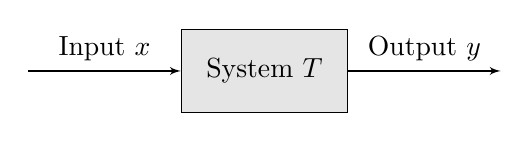
\begin{tikzpicture}[auto, node distance=3cm,>=latex']
    \node [input, name=input] {};
    \node [block, right of=input] (system) {System $T$};
    \node [output, right of=system] (output) {};

    \draw [draw,->] (input) -- node {Input $x$} (system);
    \draw [->] (system) -- node {Output $y$} (output);
  \end{tikzpicture}
\end{center}

This course is about the mathematical models and related techniques for the design and understanding of systems as signal transformations. We focus on a broadly useful class of systems, known as {\it linear, time-invariant systems}. You will learn about:

\begin{itemize}
\item the representation and analysis of signals as information carrying channels
\item and how to analyze and implement linear, time-invariant systems to transform those signals.
\end{itemize}

\begin{example} Electrical Circuits. This is a Sallen-Key filter, a second-order system commonly use to select frequencies from a signal:
  \begin{center}
    \begin{circuitikz}[american voltages,scale=0.8, every node/.style={transform shape}]
      \draw
      (7,3.5) node[op amp] (opamp1) {}
      (0,4) to[R,l=$R_1$,o-] (2,4)
      (2,4) to[short] (2,5)
      (2,5) to[C,l=$C_1$] (8.2,5)
      (8.2,5) to[short] (opamp1.out) 
      (2,4) to[R, l=$R_2$] (4,4)
      (4,4) to[C, l=$C_2$] (4,0)
      (0,0) to[short,o-o] (12,0)
      (4,4) to[short] (opamp1.-)
      (opamp1.+) to[short] (5.8,1.75)
      (5.8,1.75) to[short] (8.2,1.75)
      (opamp1.out) to[R, l=$(1-\beta)R$] (8.2,1.75)
      (8.2,1.75) to[R, l=$\beta R$] (8.2,0)
      (opamp1.out) to[short, -o] (12,3.5)
      (0,4) to[open, v=$x(t)$] (0,0)
      (12,3.5) to[open, v=$y(t)$] (12,0);
    \end{circuitikz}
  \end{center}
  How do we choose the values of the resistors and capacitors to select the frequencies we are interested in? How do we determine what those frequencies are?
\end{example}

\begin{example} Robotic Joint. This is a Linear, Time-Invariant model of a DC motor, a mixture of electrical and mechanical components.

  \begin{center}
    \tikzstyle{block} = [draw, fill=gray!20, rectangle, 
      minimum height=3em, minimum width=3em]
    \tikzstyle{sum} = [draw, fill=gray!20, circle, node distance=1cm]
    \tikzstyle{input} = [coordinate]
    \tikzstyle{output} = [coordinate]
    \tikzstyle{pinstyle} = [pin edge={to-,thin,black}]

    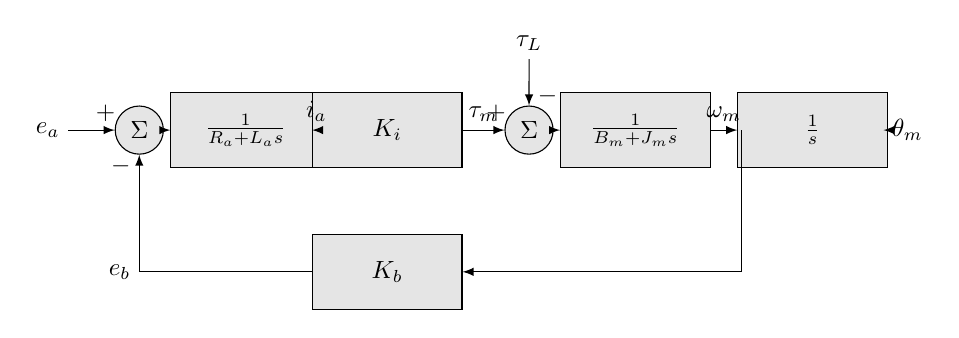
\begin{tikzpicture}[auto, node distance=2cm,>=latex, scale=0.9, every node/.style={transform shape}]

      \node [sum] at (2.5,0) (vsum) {$\Sigma$};
      \node [block] at (4,0) (arm) {$\frac{1}{R_a + L_a s}$};
      \node [block] at (6,0) (torque) {$K_i$};
      \node [sum] at (8,0) (tsum) {$\Sigma$};
      \node [block] at (9.5,0) (motor) {$\frac{1}{B_m + J_m s}$};
      \node [block] at (12,0) (int) {$\frac{1}{s}$};
      \node [block] at (6,-2) (backemf) {$K_b$};

      \draw [->] (1.5,0) node [left] {$e_a$} -- node[pos=0.8] {$+$} (vsum);
      \draw [->] (vsum) -- (arm);
      \draw [->] (arm) -- (torque) node [midway,above] {$i_a$};
      \draw [->] (torque) -- node[pos=0.8] {$+$} (tsum) node [midway,above] {$\tau_m$};
      \draw [->] (tsum) -- (motor);
      \draw [->] (8,1) node[above] {$\tau_L$} -- node[pos=0.8] {$-$} (tsum);
      \draw [->] (motor) -- (int) node [midway,above] {$\omega_m$};
      \draw [->] (11,0) |- (backemf);
      \draw [->] (backemf) -| node[midway] {$e_b$} node[pos=0.95] {$-$} (vsum);
      \draw [->] (int) -- (13,0) node[right] {$\theta_m$};
    \end{tikzpicture}
  \end{center}
  
  How do we convert the motor into a servo for use in a robotic joint? What are its characteristics (e.g. how fast can it move)?
\end{example}

\begin{example} Audio Processing. Suppose you record an interview for a podcast, but during an important part of the discussion, the HVAC turns on and there is an annoying noise in the background.

  \begin{center}
    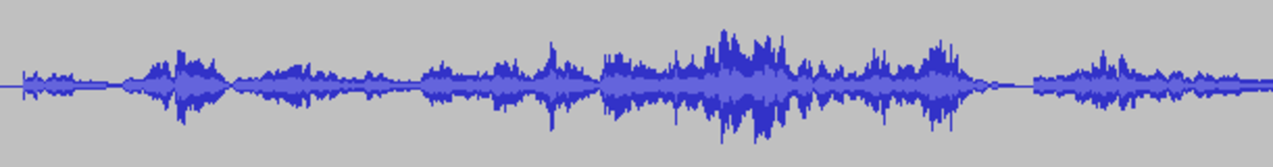
\includegraphics[scale=0.5]{figures/noisysignal.pdf}
  \end{center}

  How could you remove the noise minimizing distortion to the rest of the audio?
\end{example}

\begin{example} Communications. Consider a wireless sensor, that needs to transmit to a base station, e.g. a wireless mic system. 
  \begin{center}
    \tikzset{block/.style = {draw, fill=white, rectangle,
        minimum height=3em, minimum width=2cm},
      input/.style = {coordinate},
      output/.style = {coordinate},
      pinstyle/.style = {pin edge={to-,t,black}},
      radiation/.style={decorate,decoration={expanding waves,angle=12,segment length=4pt}}
    }
    \begin{tikzpicture}[auto, node distance=2cm,>=latex']
      \node[block](tx){Sensor Node};
      \node[antenna] at (tx.east) {};
      \node[block,right = 5cm of tx](rx){Base Station};
      \node[antenna,xscale=-1] at (rx.west) {};

      \draw[radiation] ([shift={(1cm,2cm)}]tx.east)-- node [above=5mm] {} ([shift={(-1cm,2cm)}]rx.west);
    \end{tikzpicture}
  \end{center}

  How should the signal be processed so it can be transmitted? How should the received signal be processed?
\end{example}

\subsection*{Types of Problems}
Applications of this material occur in all areas of science and engineering. When we have a measured output but are unsure what combination of inputs and system components could have produced it, we have a {\it modeling} problem.

\begin{center}
  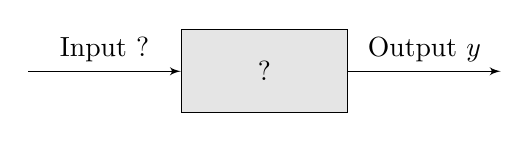
\begin{tikzpicture}[auto, node distance=3cm,>=latex']
    \node [input, name=input] {};
    \node [block, right of=input] (system) {?};
    \node [output, right of=system] (output) {};

    \draw [draw,->] (input) -- node {Input ?} (system);
    \draw [->] (system) -- node {Output $y$} (output);
  \end{tikzpicture}
\end{center}

Models are the bedrock of the scientific method and are required to apply the concepts of this course to engineering problems. 

When we know the input and the system description and desire to know the output we have an {\it analysis} problem. 

\begin{center}
  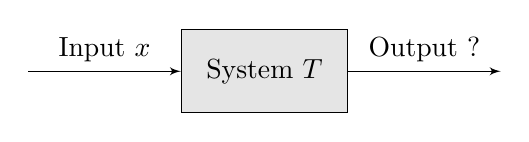
\begin{tikzpicture}[auto, node distance=3cm,>=latex']
    \node [input, name=input] {};
    \node [block, right of=input] (system) {System $T$};
    \node [output, right of=system] (output) {};

    \draw [draw,->] (input) -- node {Input $x$} (system);
    \draw [->] (system) -- node {Output ?} (output);
  \end{tikzpicture}
\end{center}

Analysis problems are the kind you have encountered most often already. For example, given an electrical circuit and an applied voltage or current, what are the voltages and currents across and through the various components.

When we know either the input and desired output and seek the system to perform this transformation,
\begin{center}
  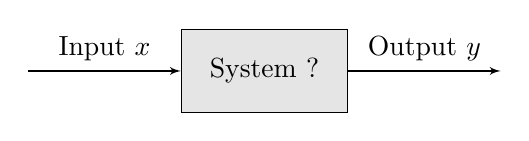
\begin{tikzpicture}[auto, node distance=3cm,>=latex']
    \node [input, name=input] {};
    \node [block, right of=input] (system) {System ?};
    \node [output, right of=system] (output) {};

    \draw [draw,->] (input) -- node {Input $x$} (system);
    \draw [->] (system) -- node {Output $y$} (output);
  \end{tikzpicture}
\end{center}

or we know the system description and output and desire the input that would generate the output,

\begin{center}
  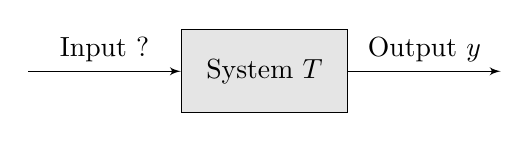
\begin{tikzpicture}[auto, node distance=3cm,>=latex']
    \node [input, name=input] {};
    \node [block, right of=input] (system) {System $T$};
    \node [output, right of=system] (output) {};

    \draw [draw,->] (input) -- node {Input ?} (system);
    \draw [->] (system) -- node {Output $y$} (output);
  \end{tikzpicture}
\end{center}

we have a {\it design problem}.

This course focuses on modeling and analysis with applications to electrical circuits and devices for measurement and control of the physical world and is broadly applicable to all ECE majors. Some Examples:

\begin{itemize}
\item Controls, Robotics, \& Autonomy: LTI systems theory forms the basis of perception and control of machines.
\item Communications \& Networking: LTI systems theory forms the basis of transmission and reception of signals, e.g. AM and FM radio.
\item Machine Learning: LTI systems are often used to pre-process samples or to create basis functions to improve learning.
\item Energy \& Power Electronic Systems: linear circuits are often modeled as LTI systems.
\end{itemize}

Subsequent courses, e.g. ECE 3704, focus more on analysis and design.

\subsection*{Learning Objectives}

The learning objectives (LOs) for the course are:
\begin{enumerate}
\item[LO-1] Describe a given system using a block-level description and identify the input/output signals.
\item[LO-2] Mathematically model continuous and discrete linear, time-invariant systems using differential and difference equations respectively.
\item[LO-3] Analyze the use of filters and their interpretation in the time and frequency domains and implement standard filters in hardware and/or software.
\item[LO-4] Apply computations of the four fundamental Fourier transforms to the analysis and design of linear systems.
\item[LO-5] Communicate solutions to problems and document projects within the domain of signals and systems through formal written documents.
\end{enumerate}

These are broken down further into the following topic learning objectives (TLOs). These are well covered in the course Textbook "Oppenheim, A. V., Willsky, A. S., and Nawab, S. H. Signals and Systems. ii, Essex UK: Prentice Hall Pearson, 1996." (abbreviated OW). This is an older, but very good book. However there are many, many texts that cover the same material. \textit{Engaged} reading the textbook is one of the most important things you can do to learn this material. Importantly, these notes should \textbf{not} be considered a replacement for the textbook.

\begin{enumerate}
\item[TLO-1] Course introduction (OW Forward and \S 1.0)
  \begin{enumerate}
  \item Signals as models
  \item Systems as transformation of signals
  \item Prerequisites
  \end{enumerate}

\item[TLO-2] Continuous-time (CT) signals (OW \S 1.1 through 1.4 and 2.5)
  \begin{enumerate}
  \item Continuous-time signals as functions $\mathbb{R}\mapsto\mathbb{C}$
  \item Transformations of time
  \item Characterizing signals
    \begin{enumerate}
    \item periodic/aperiodic
    \item even/odd
    \item energy or/nor power
    \end{enumerate}
  \item Impulse function
  \item Step function
  \item Complex exponential
  \end{enumerate}

\item[TLO-3] Discrete-time (DT) signals (OW \S 1.1 through 1.4)
  \begin{enumerate}
  \item Discrete-time signals as functions $\mathbb{Z}\mapsto\mathbb{C}$
  \item Transformations of time index
  \item Characterizing signals
    \begin{enumerate}
    \item periodic/aperiodic
    \item even/odd
    \item energy or/nor power
    \end{enumerate}
  \item Impulse function
  \item Step function
  \item Complex exponential
  \end{enumerate}

\item[TLO-4] CT systems as linear constant coefficient differential equations (OW \S 2.4.1)
  \begin{enumerate}
  \item LCCDE and their solution (1st and 2nd order)
  \item impulse response from LCCDE
  \end{enumerate}
  
\item[TLO-4] DT systems as linear constant coefficient difference equations (OW \S 2.4.2)
  \begin{enumerate}
  \item LCCDE and their solution (1st and 2nd order)
  \item impulse response from LCCDE
  \end{enumerate}
  
\item[TLO-5] Linear time invariant CT systems (OW \S 1.5, 1.6, 2.3)
  \begin{enumerate}
  \item Memory
  \item Invertability
  \item Causality
  \item Stability
  \item Time-invariance
  \item Linearity
  \item Define LTI system
  \end{enumerate}

\item[TLO-6] Linear time invariant DT systems (OW \S 1.5, 1.6, 2.3)
  \begin{enumerate}
  \item Memory
  \item Invertability
  \item Causality
  \item Stability
  \item Time-invariance
  \item Linearity
  \item Define LTI system
  \end{enumerate}

\item[TLO-7] CT convolution (OW \S 2.2)
  \begin{enumerate}
  \item Review CT LTI systems and superposition property
  \item CT Convolution Integral
  \item Properties of convolution
    \begin{enumerate}
    \item communative 
    \item distributive
    \item associative
    \end{enumerate}
  \item Determining system response using convolution with impulse response
  \end{enumerate}

\item[TLO-8] DT convolution (OW \S 2.1)
  \begin{enumerate}
  \item Review DT LTI systems and superposition property
  \item DT Convolution Sum
  \item Properties of convolution
    \begin{enumerate}
    \item communative 
    \item distributive
    \item associative
    \end{enumerate}
  \item Determining system response using convolution with impulse response
  \end{enumerate}
  
\item[TLO-9] CT block diagrams (OW \S 1.5.2 and 2.4.3)
  \begin{enumerate}
  \item blocks represented by impulse response
  \item series and parallel connections, reductions
  \item scale, sum, and integrator blocks
  \item equivalence of LCCDE's and block diagrams
  \item first-order differential equation as feedback motif
  \item second-order differential equation as a feedback motif
  \item implementing a LCCDE using adders, multipliers, and integrators
  \end{enumerate}

\item[TLO-10] DT block diagrams (OW \S 1.5.2 and 2.4.3)
  \begin{enumerate}
  \item blocks represented by impulse response
  \item series and parallel connections, reductions
  \item scale, sum, and unit delay blocks
  \item equivalence of LCCDE's and block diagrams
  \item first-order difference equation as feedback motif
  \item second-order difference equation as a feedback motif
  \item implementing a LCCDE using adders, multipliers, and delays
  \end{enumerate}

\item[TLO-11] Eigenfunctions of CT systems (OW \S 3.2 and 3.8)
  \begin{enumerate}
  \item Eigenfunction $e^{st}$
  \item Transfer Function $H(s)$
  \item Stability and Frequency Response (FR)  $H(j\omega)$
  \item How this is useful - decomposition of input signal into complex exp
  \item What signals can be decomposed this way, foreshadow Fourier Analysis
  \end{enumerate}
  
\item[TLO-12] Eigenfunctions of DT systems (OW \S 3.2 and 3.8)
  \begin{enumerate}
  \item Eigenfunction $z^{n}$
  \item Transfer Function $H(z)$
  \item Stability and Frequency Response (FR) $H\left(e^{j\omega}\right)$
  \item How this is useful - decomposition of input signal into complex exp
  \item What signals can be decomposed this way, foreshadow Fourier Analysis
  \end{enumerate}
  
\item[TLO-13] CT Fourier Series representation of signals (OW \S 3.3 through 3.5)
  \begin{enumerate}
  \item review CT periodic functions
  \item harmonic sums
  \item derive synthesis equation
  \item derive analysis equation
  \item spectrum plots
  \item define mean-square convergence
  \item truncated CT FS
  \item stable LTI system response using CTFS
  \item example of the impulse train (for sampling theory later)
  \item formal Dirichlet conditions
  \item properties of CT FS
  \end{enumerate}

\item[TLO-14] DT Fourier Series representation of signals  (OW \S 3.6 and 3.7)
  \begin{enumerate}
  \item review DT periodic functions
  \item harmonic sums
  \item derive synthesis equation
  \item derive analysis equation
  \item spectrum plots
  \item stable LTI system response using DTFS
  \item properties of DT FS
  \end{enumerate}
  
\item[TLO-15] CT Fourier Transform (OW \S 4.0 through 4.7)
  \begin{enumerate}
  \item derive the CTFT pair from the CTFS 
  \item Dirichlet existence conditions
  \item CTFT of the CTFS
  \item Properties of the CT Fourier Transform
    \begin{enumerate}
    \item linearity
    \item time shift
    \item conjugacy
    \item integration and differentiation: application to LCCDE $\mapsto$ CTFR
    \item time scaling
    \item duality
    \item convolution: stable LTI system response using CTFT
    \item multiplication/modulation
    \item application of the properties in combination
    \end{enumerate}
  \end{enumerate}

\item[TLO-16] DT Fourier Transform (OW \S 5.0 though 5.8)
  \begin{enumerate}
  \item derive the DTFT from DTFS
  \item DTFT of DTFS
  \item Properties of the DT Fourier Transform
    \begin{enumerate}
    \item periodicity
    \item linearity
    \item index-shift: application to LCCDE $\mapsto$ DTFR
    \item frequency shift
    \item conjugation
    \item finite difference and accumulation
    \item interpolation /index expansion
    \item frequency differentiation
    \item Parseval's
    \item convolution: stable LTI system response using DTFT
    \item multiplication/modulation
    \item application of the properties in combination
    \end{enumerate}
  \end{enumerate}

\item[TLO-17] CT Frequency Response (OW \S 6.1, 6.2, 6.5)
  \begin{enumerate}
  \item review CTFR as CTFT of impulse response
  \item review CTFR to/from LCCDE
  \item review CTFR to/from block diagram 
  \item magnitude-phase representation of the frequency response
  \item frequency response acting on sinusoids
  \item Bode plots
    \begin{enumerate}
    \item why plot it this way: dB units and log time axis
    \item how to read them (\textbf{not} construct them manually)
    \item Bode plots in software, e.g. Matlab/Python/Julia
    \end{enumerate}
  \item CTFR of first and second order systems
  \end{enumerate}

\item[TLO-18] DT Frequency Response (OW \S 6.1, 6.2, 6.6)
  \begin{enumerate}
  \item review DTFR as DTFT of impulse response
  \item review DTFR to/from LCCDE
  \item review DTFR to/from block diagram 
  \item magnitude-phase representation of the frequency response
  \item frequency response acting on sinusoids
  \item DTFR plots  
    \begin{enumerate}
    \item periodicity
    \item dB units
    \item DTFR plots in software, e.g. Matlab/Python/Julia
    \end{enumerate}
  \item DTFR of first and second order systems
  \end{enumerate}
  
\item[TLO-19] Frequency Selective Filters in CT (OW \S 3.9, 3.10, 6.3, 6.4) 
  \begin{enumerate}
  \item ideal low-pass
  \item ideal high-pass
  \item ideal bandpass
  \item ideal notch/bandstop
  \item practical filters
  \item transformations
  \item first and second order systems as building blocks
    \begin{enumerate}
    \item review LCCDE representation
    \item review block diagram representation
    \item review CTFR representation
    \item CT 1st order RC+buffer
    \item CT Sallen-key
    \end{enumerate}
  \end{enumerate}
  
\item[TLO-20] Frequency Selective Filters in DT (OW \S 3.11, 6.3, 6.4)
  \begin{enumerate}
  \item ideal low-pass
  \item ideal high-pass
  \item ideal bandpass
  \item ideal notch/bandstop
  \item practical filters
  \item transformations
  \item first and second order systems as building blocks
    \begin{enumerate}
    \item review LCCDE representation
    \item review block diagram representation
    \item review DTFR representation
    \item DT 1st order implementation in code
    \item DT 2nd order implementation in code
    \end{enumerate}
  \end{enumerate}
  
\item[TLO-21] The Discrete Fourier Transform
  \begin{enumerate}
  \item time window the DTFT to get the DFT
  \item interpreting the index axis as DT and CT frequency
  \item zero-padding
  \item offline or batched filtering using the DFT
  \item briefly mention fast algorithms to compute the DFT = FFT
  \end{enumerate}
  
\item[TLO-22] Sampling (OW \S 7.1, 7.3, 7.4)
  \begin{enumerate}
  \item sampling using the impulse train
  \item derive the Nyquist rate
  \item effects of aliasing
  \item practical ADC (sample and hold, SAR, bit-width)
  \item designing anti-aliasing filters
  \end{enumerate}

\item[TLO-23] Reconstruction (OW \S 7.2)
  \begin{enumerate}
  \item reconstruction as removal of images
  \item reconstruction as interpolation
  \item practical DAC: R-2R ladder
  \item designing reconstruction filters
  \end{enumerate}
\end{enumerate}

\subsection*{Graphical Outline}

\begin{center}
  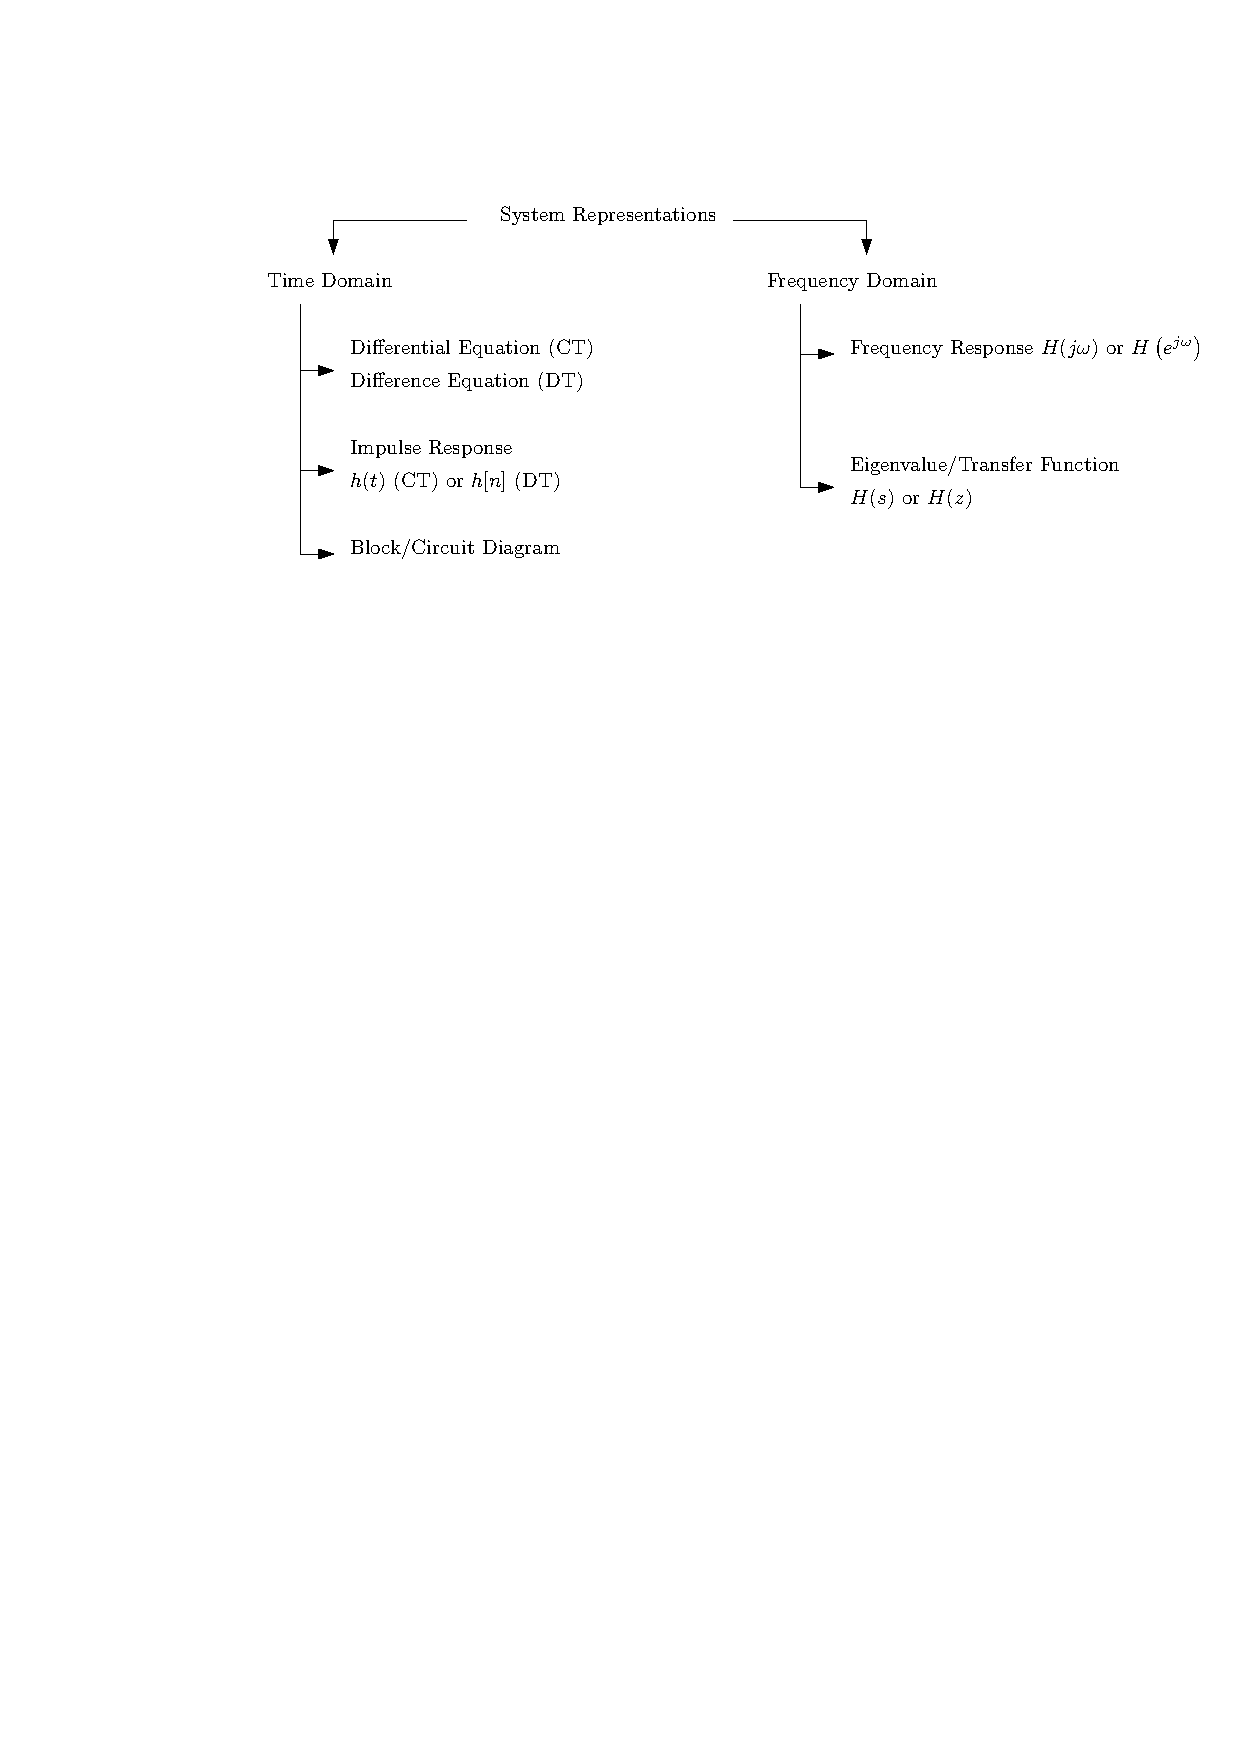
\includegraphics[scale=1]{graphics/system-representations-fig.pdf}
\end{center}
\begin{center}
  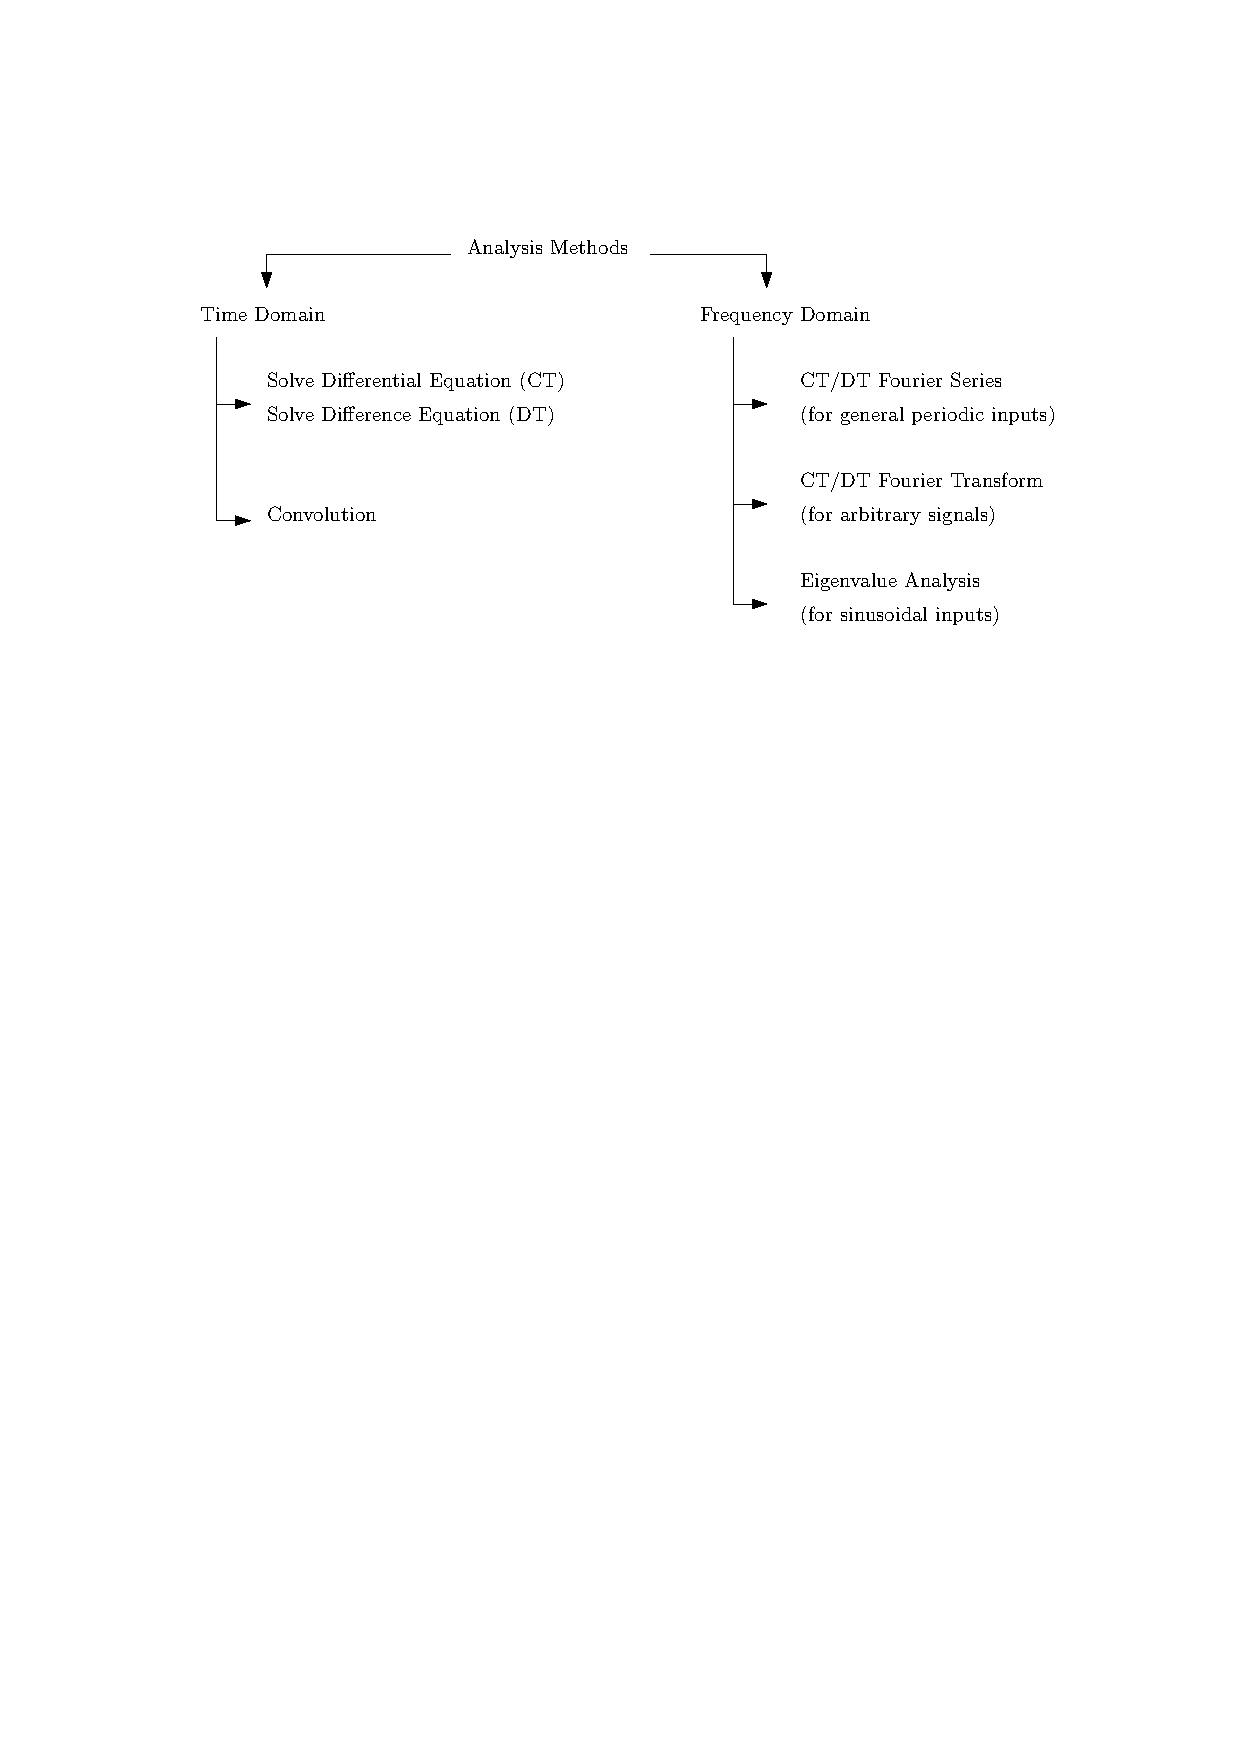
\includegraphics[scale=1]{graphics/analysis-methods-fig.pdf}
\end{center}

\newpage
\section{Prerequisites}

This course uses many concepts from prerequisite courses, particularly those from calculus and circuits. While we assume you know this material, the following sections offer a review of the most pertinent and establish some notation. If you have trouble with any of them seek assistance -- the sooner the better.

\subsection{Complex Numbers}

Complex numbers are used extensively throughout the course. You need to be very adept at manipulating them.

\subsubsection*{The Number System}

By way of review and to motivate the discussion of complext numbers, recall the following basic facts.

\begin{itemize}
\item The \emph{Natural Numbers} $\mathbb{N}$ are the positive integers $1,2,3,4,\cdots$. Given two natual numbers $a$ and $b$ the sum $a+b$ and the product $a\,b$ are also natural numbers, that is the set of natural numbers is \emph{closed} under addition and multiplication.

\item Solving equations of the form $x + a = b$ for any natural numbers $a,b$ requires the introduction of the negative integers $\cdots, -4, -3, -2 -1$ and $0$. These plus the natural numbers give the \emph{integers}  $\mathbb{Z}$. Note $\mathbb{N} \subset \mathbb{Z}$. Zero ($0$) is called the identity element with respect to addition, while $1$ is the identity with respect to multiplication, that is $a+0 = a$ and $ a \cdot 1 = a$. The \emph{inverse} of an integer $a$ is $-a$, such that thier sum gives the identity for addition, i.e. $a + -a = 0$.

\item The \emph{rational numbers} $\mathbb{Q}$ are of the form $\frac{b}{a}$ for integers $a,b$ with $a \neq 0$. They solve problems of the form $ax=b$ and provide the inverse for multiplication since $\frac{1}{a} \cdot a = 1$. Note $\mathbb{Z} \subset \mathbb{Q}$

\item The \emph{irrational numbers} are those that cannot be written as a rational number, for example $\sqrt{2} = 1.414\ldots$ and $\pi = 3.14159\ldots$

\item The union of the rational and irrational numbers give the \emph{real numbers} denoted $\mathbb{R}$.
\end{itemize}

Graphically the numbers and thier ordering can be expressed using the number line:

\begin{center}
  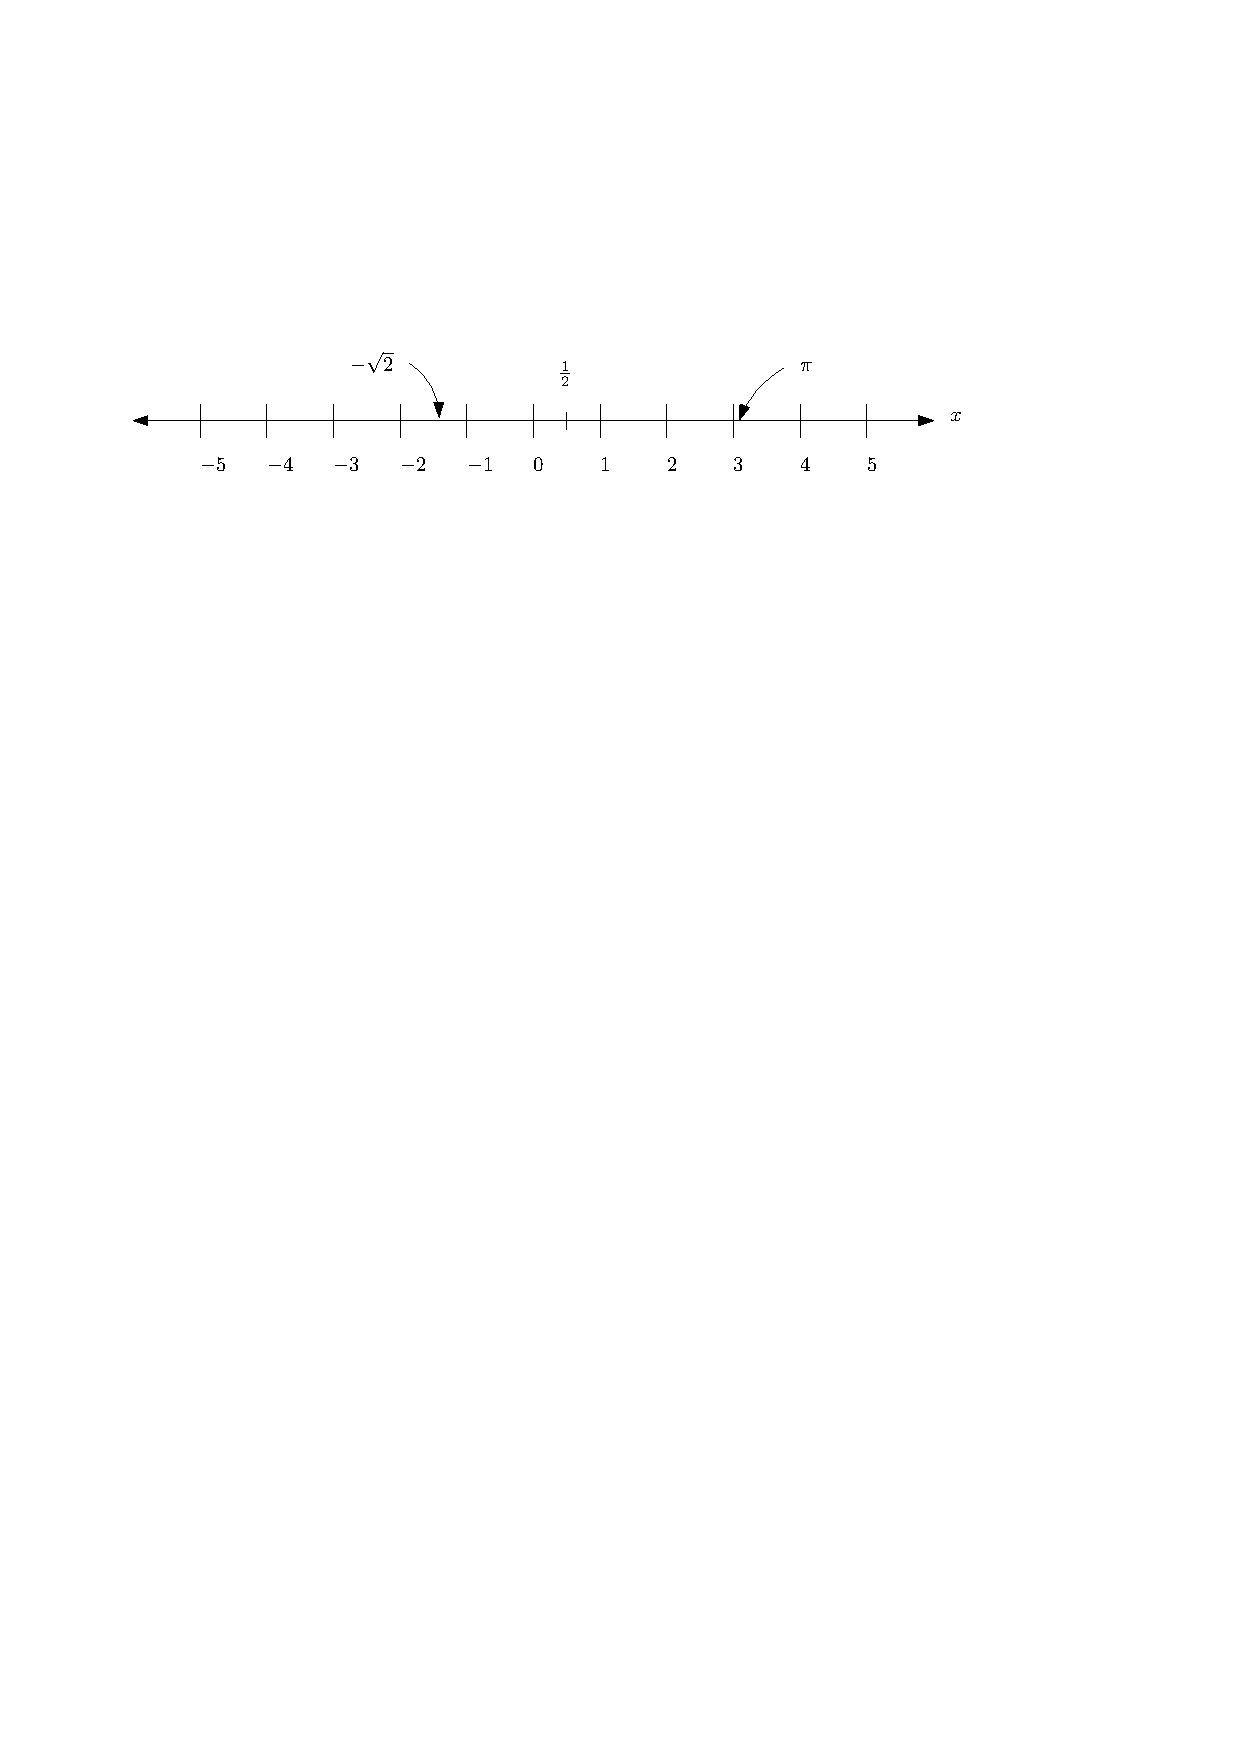
\includegraphics[scale=1]{graphics/number-line.pdf}
\end{center}

\subsubsection*{Complex numbers as extension of reals}

Continuing the pattern of the basic number system we can ask what are solutions of equations of the form $x^2+a = 0$ or $x^2 + 2ax +a^2 + b^2 = 0$ for $a,b \in \mathbb{R}$ ? As above, finding such solutions requires moving to a larger set of numbers, the \emph{complex numbers} denoted $\mathbb{C}$.

A complex variable $z\in\mathbb{C}$ can be written as $z = a + j\, b$ for $a,b\in\mathbb{R}$, where $j$ is the imaginary unit and $j^2 = -1$. Note in mathematics the imaginary unit is denoted $i$; this difference is purely historical. Some basic definitions:

\begin{itemize}
\item the \emph{real part} $\Re(z) = \text{Re}(z) = a$
\item the \emph{imaginary part} $\Im(z) = \text{Im}(z) = b$
\item two complex numbers $z_1, z_2\in \mathbb{C}$ are equal if $\text{Re}(z_1) = \text{Re}(z_2)$ and $\text{Im}(z_1) = \text{Im}(z_2)$
\item $\mathbb{R} \subset \mathbb{C}$, when $b = 0$ and we say that the number is purely real
\item if $a = 0$ we say the number is purely imaginary
\item the \emph{complex conjugate} of $z = a + jb$ is $z^* = a - jb$.
\end{itemize}

\subsubsection*{Operations on complex numbers}

Arithmetic operations on complex numbers are defined using the algebra of real numbers, replacing $j^2 = -1$. Given complex numbers $a + j\, b$ and $c + j\, d$

\begin{description}
\item[addition] $(a + jb) + (c +jd) = (a+c) + j(b+d)$
\item[subtraction] $(a + jb) - (c +jd) = (a-c) + j(b-d)$
\item[multiplication] $(a + jb)\cdot(c +jd) = ac + jbc + jad + j^2 bd = (ac-bd) + j(bc+ad)$
\item[division] $\frac{(a + jb)}{(c +jd)} = \frac{ac+jbc-jad-j^2 bd}{c^2 -j^2 d^2} = \frac{(ac+bd) + j(bc-ad)}{c^2 + d^2} = \frac{ac+bd}{c^2 + d^2} + j \frac{bc-ad}{c^2 + d^2}$
\end{description}


\subsubsection*{Basic properties of complex numbers}

Let $z_1, z_2, z_3 \in \mathbb{C}$, then:

\begin{description}
\item[closure property] $z_1 + z_2 \in \mathbb{C}$ and  $z_1 \cdot z_2 \in \mathbb{C}$ 
\item[communative property] $z_1 + z_2 = z_2 + z_1$ and $z_1 \cdot z_2 = z_2 \cdot z_1$ 
\item[associative property] $z_1 + (z_2 + z_3) = (z_1 + z_2) + z_3$ and $z_1 \cdot (z_2 \cdot z_3) = (z_1 \cdot z_2) \cdot z_3$ 
\item[identity elements] $0 = (0 + j0) \in \mathbb{C}$ is the identity element for addition since $z_1 + 0 = z_1$ and $1 = 1 + j0 \in \mathbb{C}$ is the identity element for multiplication since $z_1\cdot 1 = z_1$ 
\item[inverse elements] for any $z_1$ there exists an inverse $z_2 = -z_1$ such that $z_1 + z_2 = 0$, and for any $z_1 \neq 0$ there exists an inverse $z_2 = z_1^{-1} = \tfrac{1}{z_1}$ such that $z_1 \cdot z_2 = 1$
\end{description}

\subsubsection*{Absolute Value (Magnitude) of complex numbers}

The absolute value or \textit{magnitude} of a complex number $z = a + jb$ is denoted $|z| = |a+jb|$ and is given by
\[
|a + jb| = \sqrt{a*2 + b^2}
\]
For complex numbers $z_1, z_2, \ldots, z_n$, the following useful properties hold
\begin{itemize}
\item $|z_1\cdot z_2 \cdots z_N| = |a_1|\cdot |z_2|\cdots|z_N|$
\item $\left| \frac{z_1}{z_2}\right| = \frac{|z_1|}{|z_2|}$ for $z_2 \neq 0$
\end{itemize}

\subsubsection*{Argument (Angle) of complex numbers}
The argument or \textit{angle} of a complex number $z = a + jb$ is denoted $\angle z = \angle(a+jb)$ and is given by
\[
\angle(a + jb) = \arctan\frac{b}{a}
\]
Take care when computing this number on your calculator (or in a programming language) so that it produces and angle in radians and in the correct quadrant. For example $\angle(-1-j1) = \arctan\frac{-1}{-1} = \frac{5\pi}{4} = -\frac{3\pi}{4}$ is different from $\angle(-1-j1) = \arctan\frac{-1}{-1} = \arctan\frac{1}{1} = \frac{\pi}{4}$, the later being incorrect.

\subsubsection*{Cartesian and Polar representation of complex numbers}

A complex number $z$ can be represented in Cartesian form as a pair of numbers in the \textit{Complex Plane}, $(\Re{z},\Im{z})$. The same $z$ can be represented in polar form as $z = |z|\cdot e^{j\angle z}$. We can convert between the representations using  $\Re{z} = |z| \cos(\angle z)$ and $\Im{z} = |z| \sin(\angle z)$. The following relations hold

\begin{itemize}
\item Multiplication by $j$ is equivalent to rotation by $\tfrac{\pi}{2}$
\[
j\cdot z = e^{j\tfrac{\pi}{2}}\cdot |z|\cdot e^{j\angle z} = |z|\cdot e^{j(\angle z + \tfrac{\pi}{2})} 
\]
\item Division by $j$ is equivalent to rotation by $- \tfrac{\pi}{2}$
\[
\frac{1}{j}\cdot z = e^{-j\tfrac{\pi}{2}}\cdot |z|\cdot e^{j\angle z} = |z|\cdot e^{j(\angle z - \tfrac{\pi}{2})} 
\]
\end{itemize}

A related expression that will be very useful to us is \textit{Eulers formula}: $e^{j\theta} = \cos(\theta) + j\sin(\theta)$. From this we can derive the relations:
\[
\cos(\theta) = \frac{1}{2} e^{j\theta} + \frac{1}{2} e^{-j\theta} 
\]
\[
\sin(\theta) = \frac{1}{2j} e^{j\theta} - \frac{1}{2j} e^{-j\theta} 
\]

These representations and relations can be visualized as follows
\begin{center}
  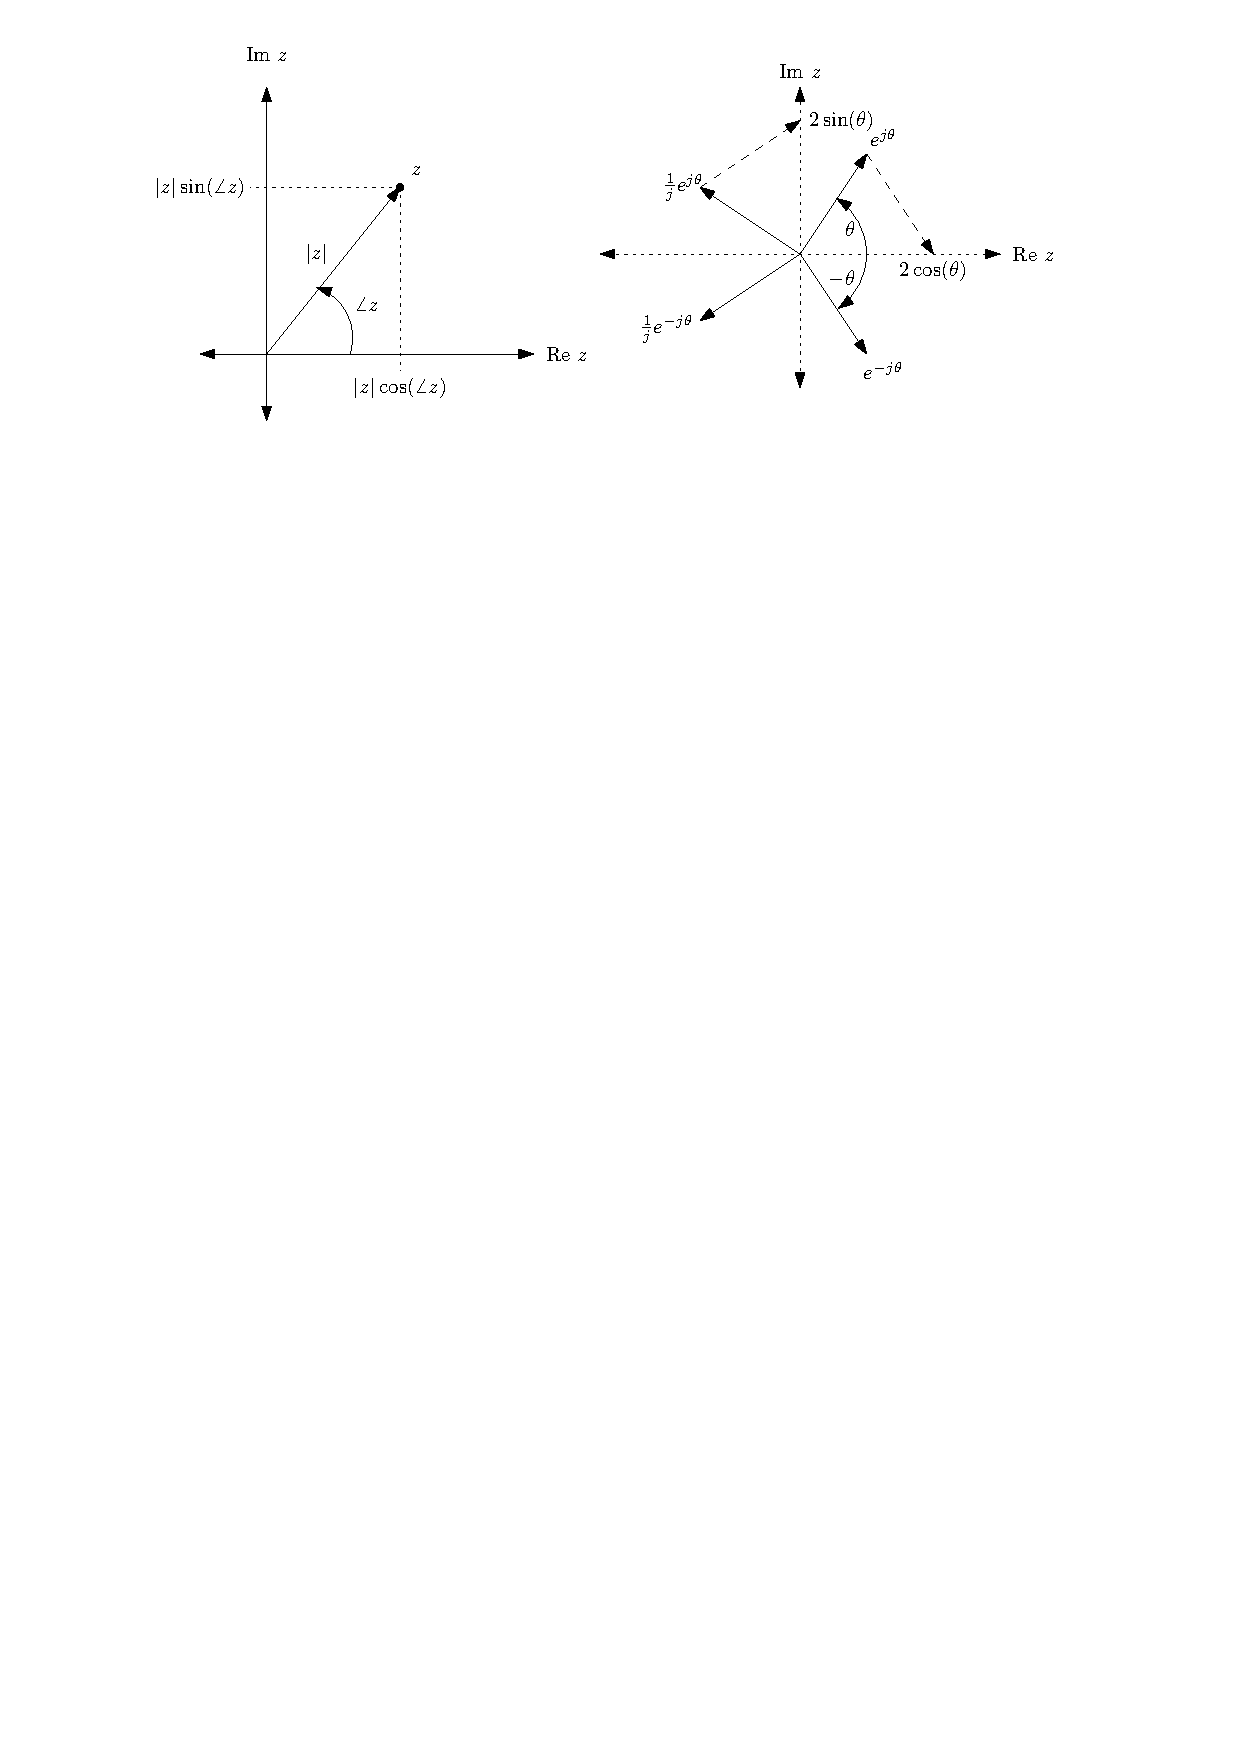
\includegraphics[scale=1]{graphics/complex-viz-prereq.pdf}
\end{center}

\subsubsection*{Complex numbers as roots of polynomial equations}

Recall our original motivation for complex numbers, as solutions to polynomials. Consider the $N^\text{th}$ order polynomial
\[
z^N + a_N z^{N-1} + \cdots + a_2 z + a_1 
\]
where in cases of interest to us in this course the $N$ coefficients $a_{N}, \cdots, a_1$ are real. In such cases the polynomial can be factored into
\[
z^N + a_{N} z^{N-1} + \cdots + a_2 z + a_1 = (z-z_1)\cdot(z-z_2)\cdots(z-z_N)
\]
where the $z_i$ are the $N$ \textit{roots} of the polynomial. These are complex numbers in general with two cases:

\begin{itemize}
\item the root is real
\item the root is complex or purely imaginary, in which case they come in congugate pairs 
\end{itemize}

Note: the \texttt{roots} function in Matlab can be used to find the roots of any order polynomial given a vector of coefficients.

\subsection{Calculus}

Calculus is used heavily in the course. Here we remind ourselves of some basic facts. Consult your calculus text for more details.

\subsubsection*{Functions}

A function is a mapping between sets
\[
f: A \rightarrow B
\]
where $A$ is a set called the {\it domain} and $B$ is a set called the {\it co-domain}. In this course we are primarily concerned with four kinds of functions

\begin{itemize}
\item the real-valued functions of an integer variable $f:\mathbb{Z}\mapsto\mathbb{R}$
\item the complex-valued functions of an integer variable $f:\mathbb{R}\mapsto\mathbb{C}$
\item the real-valued functions of a real variable $f:\mathbb{R}\mapsto\mathbb{R}$
\item the complex-valued functions of a real variable $f:\mathbb{R}\mapsto\mathbb{C}$
\end{itemize}
We will also briefly discuss the the complex-valued functions of a complex variable $f:\mathbb{C}\mapsto\mathbb{C}$.

\subsubsection*{Visualizing Functions}

You are certainly familiar with the graph of functions $f:\mathbb{R}\mapsto\mathbb{R}$. To graph a complex-valued function of a single variable we need to plot two functions. Consider a function $z(t) \in \mathbb{C}$ for $t \in \mathbb{R}$ expressed in Cartesian form:
\[
z(t) = z_r(t) + j z_i(t) 
\]
where $z_r(t) = \Re(z(t))$ and $z_r(t) = \Im(z(t))$ are the real and imaginary parts of the complex value at a given $t$. We can plot these two real-valued functions to visualize the complex function. Similarly consider a function $z(t) \in \mathbb{C}$ for $t \in \mathbb{R}$ expressed in polar form:
\[
z(t) = z_m(t) e^{jz_a(t)}
\]
where $z_m(t) = |z(t)|$ and $z_a(t) = \angle z(t)$ are the magnitude and angle of the complex value at a given $t$. We can plot these two real-valued functions to visualize the complex function.

Another approach to visualizing a complex number is to plot it as the tip of a vector that moves as a function of the independent variable.

\begin{example} Consider the function $z(t) = e^{|t| + j2t}$. Lets convert it to polar and Cartesian form
  \begin{align*}
    z(t) &=  e^{|t| + j2t}\\
    &=  \underbrace{e^{|t|}}_{z_m(t)} e^{j\overbrace{2t}^{z_a(t)}}\\
    &=  e^{|t|} (\cos(2t) + j\sin(2t))\\
    &=  \underbrace{e^{|t|}\cos(2t)}_{z_r(t)} + j \underbrace{e^{|t|}\sin(2t)}_{z_i(t)}
  \end{align*}
  We can then visualize the function as plots of the real and imaginary functions,

  \begin{tabular}{cc}
  \begin{tikzpicture}
    \begin{axis}[xmin=-5, xmax=5, ymin = -1, ymax=1, samples=1000, xlabel=$t$, ylabel=$z_r(t)$]
      \addplot[blue, thick] (x,(cos(2*180*x/pi)*cos(2*180*x/pi)));
      \addplot[mark=none, black] coordinates {(0,-1) (0,1)};
      \addplot[mark=none, black] coordinates {(-5,0) (5,0)};
    \end{axis}
  \end{tikzpicture}
  &
  \begin{tikzpicture}
    \begin{axis}[xmin=-5, xmax=5, ymin = -10, ymax=10, samples=10, xlabel=$t$, ylabel=$z_i(t)$]
      \addplot[blue, thick] (x,2*x));
      \addplot[mark=none, black] coordinates {(0,-10) (0,10)};
      \addplot[mark=none, black] coordinates {(-5,0) (5,0)};
    \end{axis}
  \end{tikzpicture}
  \end{tabular}\\
  or the mangitude and angle functions,\\
  \begin{tabular}{cc}
  \begin{tikzpicture}
    \begin{axis}[xmin=-5, xmax=5, ymin = 0, ymax=1, samples=1000, xlabel=$t$, ylabel=$z_m(t)$]
      \addplot[blue, thick] (x,e^(-abs(x)));
      \addplot[mark=none, black] coordinates {(0,0) (0,1)};
      \addplot[mark=none, black] coordinates {(-5,1) (5,1)};
    \end{axis}
  \end{tikzpicture}
  &
  \begin{tikzpicture}
    \begin{axis}[xmin=-5, xmax=5, ymin = -10, ymax=10, samples=10, xlabel=$t$, ylabel=$z_a(t)$]
      \addplot[blue, thick] (x,2*x));
      \addplot[mark=none, black] coordinates {(0,-10) (0,10)};
      \addplot[mark=none, black] coordinates {(-5,0) (5,0)};
    \end{axis}
  \end{tikzpicture}
  \end{tabular}
\end{example}


\subsubsection*{Derivatives of real-valued functions}

For functions $f:\mathbb{R}\mapsto\mathbb{R}$ recall the derivative is the rate of change in the value as a function of the independent variable, and can be defined using a limit of a difference. Consider such a function $f(t)$ for $t\in\mathbb{R}$, it's derivative is given using a forward difference:

\[
\frac{df}{dt} (t) = \lim_{h->0} \frac{f(t+h)-f(t)}{h}
\]

Higher-order derivative are defined recursively. For example, the second derivative is

\[
\frac{d^2f}{dt^2} = \lim_{h->0} \frac{\frac{df}{dt}(t+h)-\frac{df}{dt}(t)}{h}
\]
In the general case the $N^\text{th}$ order derivative is
\[
\frac{d^Nf}{dt^N} = \lim_{h->0} \frac{\frac{d^{N-1}f}{dt^{N-1}}(t+h)-\frac{d^{N-1}f}{dt^{N-1}}(t)}{h}
\]

Note there are several different notations for derivatives, e.g. $\frac{df}{dt} = f^\prime (t) = \dot{f}(t)$, but we will use the former in most cases. We will also use the derivative operator notation $\frac{d^Nf}{dt^N} = (D^N f)(t)$, which is convenient for higher-order derivatives.

A function with finite derivatives for all values of the independent variable is called \textit{continuous}. Values of the independent variable where the derivative is not finite are called \textit{discontinuities}. A function with a finite number of discontinuities is called \textit{piecewise continuous}.

\subsubsection*{Integrals of real-valued functions}

\subsection{Differential Equations}

This course assumes a background in basic differential equations. However, we use only consider linear, constant-coefficient differential equations.

\subsubsection*{linear, constant-coefficient differential equations, homogeneous and particular solutions}

Recall,

\subsection{Circuits}

ECE 2024 is required for knowledge of continuous signals representation as voltages and currents, and the analysis and construction of circuits containing resistors, capacitors, inductors, and operational amplifiers.

\begin{itemize}
\item $v = iR$\hspace{2em}
  \begin{circuitikz}[american voltages,scale=0.8, every node/.style={transform shape}]
    \draw
    (0,0) to[R,l=$R$] (4,0);
  \end{circuitikz}
  
\item $i = Cv^\prime$ \hspace{2em}
  \begin{circuitikz}[american voltages,scale=0.8, every node/.style={transform shape}]
    \draw
    (0,0) to[C,l=$C$] (4,0);
  \end{circuitikz}
\item $v = Li^\prime$ \hspace{2em}
  \begin{circuitikz}[american voltages,scale=0.8, every node/.style={transform shape}]
    \draw
    (0,0) to[L,l=$L$] (4,0);
  \end{circuitikz}
\item KVL
\item KCL
\item Ideal Op-Amp
\end{itemize}

\subsubsection*{KVL}

\subsubsection*{KCL}

\subsubsection*{Ideal OpAmps}

\subsubsection*{from circuit to differential equation}

\subsubsection*{using LiaB and building/measuring circuits}

\subsection{Programming}

ECE 2514 is required for the ability to model and simulate physical systems using computational tools, and basic programming ability.

\begin{itemize}
\item Matlab for general computation and plotting
\item C++ (a small subset) for implementing digital filters
\end{itemize}

\subsubsection*{plotting and vizualization with Matlab/Python/Julia}

\subsubsection*{Computation with C or C++}

\subsection{Digitial Systems}

ECE 2544 is required for for knowledge of digital signal representation and the analysis and construction of circuits containing combinatorial and sequential logic.

\subsubsection*{binary representation of integers vs floating point}

\subsubsection*{shift registers}

\subsubsection*{adders and multipliers}

\newpage
\section{Continuous-time Signals}

A continuous-time (CT) signal is a function of one or more independent variables conveying information about a physical phenomena. This lecture gives an introduction to continuous-time signals as functions. You learn how to characterize such signals in a number of ways and are introduced to two very important signals: the unit impulse and the complex exponential.

\subsection{Signals as Functions}

In order to reason about signals mathematically we need a representation or {\it model}. Signals are modeled as functions, mappings between sets
\[
f: A \rightarrow B
\]
where $A$ is a set called the {\it domain} and $B$ is a set called the {\it co-domain}.

The most basic classification of signals depends on the sets that makeup the domain and co-domain. We will be interested in two versions of the domain, the reals denoted $\mathbb{R}$ and the integers denoted $\mathbb{Z}$. We will be interested in two versions of the co-domain, the reals $\mathbb{R}$ and the set of complex numbers $\mathbb{C}$.

\begin{definition}[Analog Signal]
  If the function $f: \mathbb{R} \rightarrow \mathbb{R}$, we call this an analog or real, continuous-time signal, e.g. a voltage at time $t \in \mathbb{R}$, $v(t)$. We will write these as $x(t)$, $y(t)$, etc. The units of $t$ are seconds. Fig.~\ref{fig:ctplots} shows some graphical representations, i.e. plots.
\end{definition}

\begin{figure}[ht]
  \begin{center}
  \frame{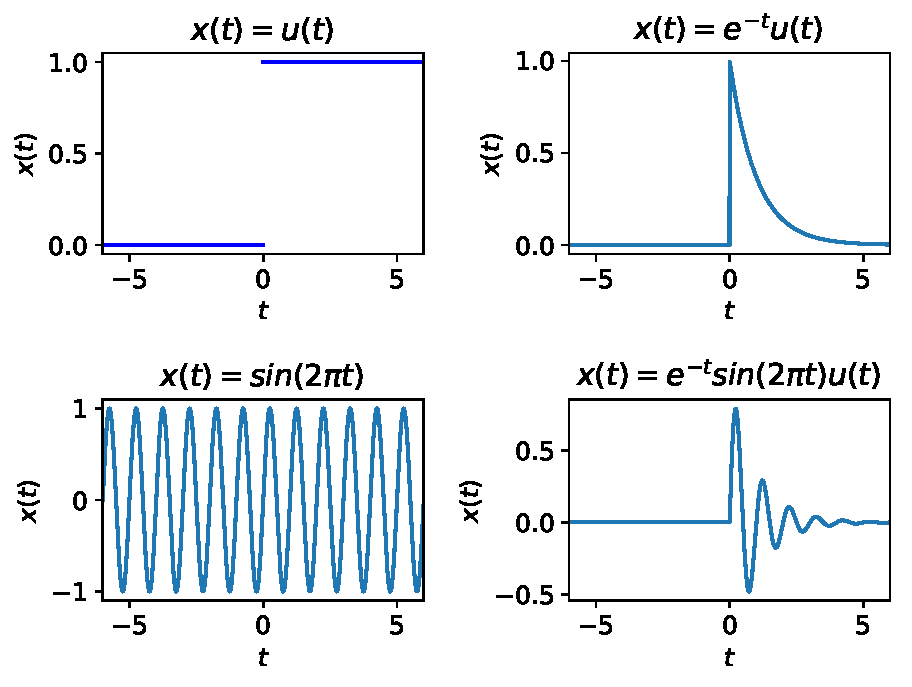
\includegraphics[scale=0.5]{graphics/ctsignals.pdf}}
  \end{center}
  \caption{Example plots of analog signals.}
  \label{fig:ctplots}
\end{figure}

\begin{definition}[Real, Discrete-time Signal]
  If the function $f: \mathbb{Z} \rightarrow \mathbb{R}$, we call this a real, discrete-time signal, e.g. the temperature every day at noon. We will write these as $x[n]$, $y[n]$, etc. Note $n$ is dimensionless.
\end{definition}

\begin{figure}[ht]
  \begin{center}
    \frame{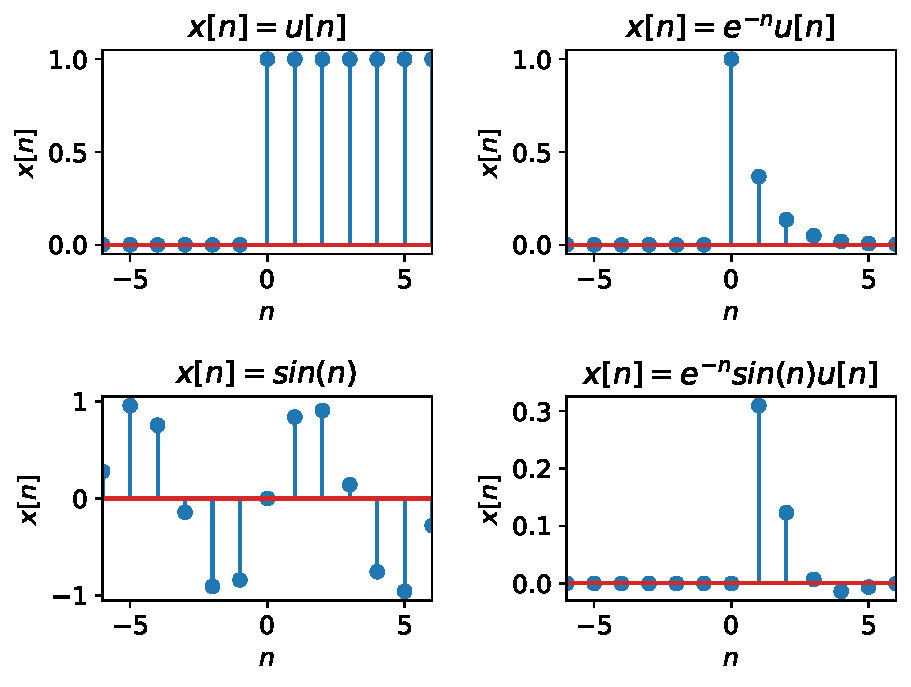
\includegraphics[scale=0.5]{graphics/dtsignals.pdf}}
  \end{center}
  \caption{Example plots of real discrete-time signals.}
  \label{fig:dtplots}
\end{figure}

Some other possibilities:
  
\begin{itemize}
\item $f: \mathbb{R} \rightarrow \mathbb{Z}$, digital, continuous-time signals, e.g. the output of a general purpose pin on a microcontroller
\item $f: \mathbb{Z} \rightarrow \mathbb{Z}$, digital, discrete-time signals, e.g. the signal on a computer bus
\end{itemize}

The co-domain can also be complex.

\begin{itemize}
\item $f: \mathbb{R} \rightarrow \mathbb{C}$, complex-valued, continuous-time signals, e.g.\\
  \[
  x(t) = e^{j\omega t} = \cos(\omega t) + j\sin(\omega t)
  \]
\item $f: \mathbb{Z} \rightarrow \mathbb{C}$, complex-valued, discrete-time signals, e.g.\\
  \[
  x[n] = e^{j\omega n} = \cos(\omega n) + j\sin(\omega n)
  \]
\end{itemize}
  
Since the domains $\mathbb{R}$ and $\mathbb{Z}$ are usually interpreted as time, we will call these {\it time-domain} signals. In the time-domain, when the co-domain is $\mathbb{R}$ we call these real signals. All physical signals are real. However complex signals will become important when we discuss the frequency domain.

\subsection{Primitive Models}

We mathematically model signals by combining elementary/primitive functions, for example:
  
\begin{itemize}
\item polynomials: $x(t) = t$, $x(t) = t^2$, etc.
\item transendental functions: $x(t) = e^t$, $x(t) = \sin(t)$, $x(t) = \cos(t)$, etc.
\item piecewise functions, e.g.
  \[
     x(t) = \left\{  \begin{array}{cl}
       f_1(t) & t < 0\\
       f_2(t) & t \geq 0\\
     \end{array}\right.
     \]
\end{itemize}

\begin{example}[Modeling a Switch]
  Consider a mathematical model of a switch, which moves positions at time $t = 0$.

  \begin{center}
  \begin{circuitikz}[american voltages,scale=0.8, every node/.style={transform shape}]
    \draw
    (0,0) to[battery, l=$V$] (0,2.3)
    (3,2) node[spdt,xscale=-1,yscale=-1,anchor=in] (Sw) {}
    (0,2.3) to[short] (Sw.out 2)
    (Sw.out 1) to[short] (1.8,0)
    (0,0) to[short, -o] (4,0)
    (3,2) to[short, -o] (4,2)
    (4,2) to[open, v=$x(t)$] (4,0);;
  \end{circuitikz}
\end{center}

We use this model so much we give it it's own name and symbol: Unit Step, $u(t)$

    \[
     u(t) = \left\{  \begin{array}{cl}
        0 & t < 0\\
        1 & t \geq 0\\
      \end{array}\right.
  \]
  so a mathematical model of the switch circuit above would be $x(t) = V u(t)$.

  Note: some texts define the step function at $t=0$ to be $1$ or $\frac{1}{2}$. It is typically plotted like so:
  \begin{center}
    \begin{tikzpicture}[scale=0.8, every node/.style={transform shape}]
  \begin{axis}[ xlabel=$t$, axis x line=center, axis y line = center, 
    xmin=-2, xmax=2, ymin=0, ymax=1.1, x label style={at={(axis cs:2,0)},anchor=west}]
    \draw[-,blue,style={ultra thick}] (axis cs:-2,0) -- (axis cs:0,0);
    \draw[-latex,blue,style={ultra thick}] (axis cs:0,1) -- (axis cs:2,1);
  \end{axis}
\end{tikzpicture}
    \end{center}
\end{example}

\begin{example}[Pure audio tone at "middle C"]
  A signal modeling the air pressure of a specific tone might be 
  \[
  x(t) = \sin\left(2\pi (261.6) t\right)
  \]
\end{example}

\begin{example}[Chord]
    The chord "G", an additive mixture of tones at G, B, and D and might be modeled as
    \[
    x(t) = \sin\left(2\pi (392) t\right) + \sin\left(2\pi (494) t\right) + \sin\left(2\pi (293) t\right) 
    \]
    This example shows we can use addition to build-up signals to approximate real signals of interest.
\end{example}

\subsection{Basic Transformations}

We can also apply transformations to signals to increase their modeling flexibility.
  
\begin{itemize}
\item  magnitude scaling
  \[
  x_2(t) = a x_1(t)
  \]
  for $a \in \mathbb{R}$.
\item derivatives
  \[
  x_2(t) = x_1^\prime(t)
  \]
\item integrals
  \[
  x_2(t) = \int\limits_{-\infty}^t x_1(\tau) \; d\tau
  \]
\item sums
  \[
  y(t) = \sum\limits_{i} x_i(t)
  \]
  an important example we will see is the CT Fourier series.  
\item multiplication (modulation)
  \[
  y(t) = x_1(t) x_2(t)
  \]
  For example amplitude modulation $y(t) = x(t)\sin(\omega_0 t)$
\item time shift
  \[
  x_2(t) = x_1(t+\tau)
  \]
  \begin{itemize}
  \item if $\tau <0$ it is called a {\it delay}
  \item if $\tau >0$ it is called an {\it advance}
  \end{itemize}
  \item time scaling
    \[
    x_2(t) = x_1\left(\frac{t}{\tau}\right)
    \]
    \begin{itemize}
    \item if $\tau >0$ increasing $\tau$ expands in time, slows the signal
    \item if $\tau <0$ time reverses and decreasing $\tau$ expands in time
    \end{itemize}
    Example: time reversal $ x_2(t) = x_1(-t)$
\end{itemize}

\subsection{Characterization of Signals}

There are a few basic ways of characterizing signals.

\begin{definition}[Causal CT Signal]
  A CT signal is \emph{causal} if $x(t) = 0$ $\forall t < 0$.
\end{definition}
\begin{definition}[Anti-Causal CT Signal]
  A CT signal is \emph{anti-causal} or acausal if $x(t) = 0$ $\forall t \geq 0$.
\end{definition}

A signal can be written as the sum of a causal and anti-causal signal.

\begin{definition}[Periodic Signals]
  A CT signal is \emph{periodic} if $x(t) = x(t + T)$ $\forall t$ for a fixed parameter $T \in \mathbb{R}$ called the \emph{period}.
\end{definition}
  
The simplest periodic signals are those based on the sinusoidal functions.
  
\begin{definition}[Even Signal]
  A CT signal is \emph{even} if $x(t) = x(-t)$ $\forall t$.
\end{definition}

\begin{definition}[Odd Signal]
  A CT signal is \emph{odd} if $x(t) = -x(-t)$ $\forall t$. 
\end{definition}

Any CT signal can be written in terms of an even and odd component
\[
x(t) = x_e(t) + x_o(t) 
\]
where 
\[
\begin{array}{ll}
  x_e(t) &= \frac{1}{2}\left\{x(t) + x(-t)\right\} \\
  & \\
  x_o(t) &= \frac{1}{2}\left\{x(t) - x(-t)\right\}
\end{array}
\]

\begin{definition}[Energy of a CT Signal]
  The \emph{energy} of a CT signal $x(t)$ is defined as a measure of the function
  \[
  E_x = \lim_{T\rightarrow\infty} \int\limits_{-T}^T \lvert x(t) \rvert^2 dt \; .
  \]
\end{definition}

\begin{definition}[Power of a CT Signal]
  The \emph{power} of a CT signal is the energy averaged over an interval as that interval tends to infinity.
  \[
  P_x = \lim_{T\rightarrow\infty} \frac{1}{2T} \int_{-T}^T \lvert x(t)\rvert^2 dt \; .
  \]
\end{definition}

Signals can be characterized based on their energy or power:  
\begin{itemize}
\item Signals with finite, non-zero energy and zero power are called {\it energy signals}.
\item Signals with finite, non-zero power (and by implication infinite energy) are called {\it power signals}.
\end{itemize}

Note, these categories are non-exclusive, some signals are neither energy or power signals.

\subsection{Unit Impulse Function}
An important CT signal is the unit impulse function, also called the "delta" $\delta$ function for the symbol traditionally used to define it. Applying this signal to a system models a "kick" to that system. For example, consider striking a tuning fork. The reason this signal is so important is that it will turn out that the response of the system to this input tells us all we need to know about a linear, time-invariant system!

\begin{definition}[CT Impulse Function]
The CT impulse function is not really a function at all, but a mathematical object called a "distribution". Some equivalent definitions:

\[
\delta(t) = \lim_{\epsilon \rightarrow 0}\left\{
\begin{array}{ll}
  \frac{1}{2\epsilon} & |t| < \epsilon\\
  0 & \text{else}
\end{array}
\right.
\]

\[
\delta(t) = \lim_{\epsilon \rightarrow 0} \frac{1}{\sqrt{2\pi}\epsilon} e^{-\frac{t^2}{2\epsilon^2}}
\]
Note the area under each definition is always one.
\end{definition}

In practice we can often use the following definition and some properties, without worrying about the distribution functions.
\[
\delta(t) = \left\{
\begin{array}{ll}
  0 & t \neq 0\\
  \infty & t = 0
\end{array}
\right. 
\]
which we draw an vertical arrow in plots:
\begin{center}
  \begin{tikzpicture}[scale=0.8, every node/.style={transform shape}]
    \begin{axis}[ xlabel=$t$, axis x line=center, axis y line = center, 
        xmin=-2, xmax=2, ymin=0, ymax=1.1, x label style={at={(axis cs:2,0)},anchor=west}]
      \addplot+[ycomb,mark=triangle,style={ultra thick}] plot coordinates {(0,1)};
    \end{axis}
  \end{tikzpicture}
\end{center}
Note the height of the arrow is arbitrary. Often in the case of a non-unit impulse function the area is written in parenthesis near the arrow tip.

The following properties of the impulse function will be used often.

\begin{itemize}
\item The energy of the unit impulse is unity since by definition
  \[
  \int\limits_{-\infty}^{\infty} \delta(t) \; dt = 1
  \]
\item Sampling property: $x(t)\delta(t-t_0) = x(t_0)\delta(t-t_0)$
\item Sifting Property:
  \[
  \int\limits_{a}^{b} x(t)\delta(t-t_0) \; dt = x(t_0)
  \]
  for any $a < t_0 < b$.
\end{itemize}

We previously defined the unit step function. The impulse can be defined in terms of the step:
\[
\delta(t) = \frac{du}{dt}
\]
and vice-versa
\[
u(t) = \int\limits_{-\infty}^{t} \delta(\tau) \; d\tau
\]
using the notion of distributions, e.g.

\[
u(t) = \int\limits_{-\infty}^{t} \delta(\tau) \; d\tau = \lim_{\epsilon \rightarrow 0} \int\limits_{-\infty}^{t} \frac{1}{\sqrt{2\pi}\epsilon} e^{-\frac{\tau^2}{2\epsilon^2}} \; d\tau = \lim_{\epsilon \rightarrow 0} \frac{1}{2}\left(1+\text{erf}\left( \frac{t}{\sqrt{2}\epsilon}\right)\right)
\]

The step and impulse function are related, but in many cases finding the response of a system to a step input is easier.

We can apply additional transformations to the impulse and step functions to get other useful signals, e.g.

\begin{itemize}
\item ramp
  \[
  r(t) = \int\limits_{-\infty}^{t} u(\tau) \; d\tau = tu(t)
  \]
  
\item causal pulse of width $\epsilon$
  \[
  p(t) = u(t) - u(t-\epsilon)
  \]
  
\item non-causal pulse of width $2\epsilon$
  \[
      p(t) = u(t+\epsilon) - u(t-\epsilon)
      \]
\end{itemize}

\subsection{CT Complex Exponential}

One of the most important signals in systems theory is the complex exponential:
\[
x(t) = C\, e^{a t}
\]
where the parameters $C, a \in \mathbb{C}$ in general.

When $C$ and $a$ are both real ($\Im(C) = \Im(a) = 0$), we have the familiar exponential. When $a > 0$, $x(t) = C e^{a t}$ looks like:

\begin{center}   
  \begin{tikzpicture}
    \begin{axis}[xmin=-2, xmax=2, ymin = 0, ymax=7, samples=50, xlabel=$t$, xticklabels={,,}, yticklabels={,,}]
      \addplot[blue, thick] (x,e^x);
      \addplot[mark=none, black] coordinates {(0,0) (0,7)};
      \addplot[mark=none, black] coordinates {(-2,1) (2,1)};
      \node at (axis cs:0,2) [anchor=north east] {$C$};
    \end{axis}
  \end{tikzpicture}
\end{center}

When $a < 0$, $x(t) = C e^{a t}$ looks like:

\begin{center}
  \begin{tikzpicture}
    \begin{axis}[xmin=-2, xmax=2, ymin = 0, ymax=7, samples=50, xlabel=$t$, xticklabels={,,}, yticklabels={,,}]
      \addplot[blue, thick] (x,e^-x);
      \addplot[mark=none, black] coordinates {(0,0) (0,7)};
      \addplot[mark=none, black] coordinates {(-2,1) (2,1)};
      \node at (axis cs:0,2) [anchor=north east] {$C$};
    \end{axis}
  \end{tikzpicture}
\end{center}

To get the pure sinusoidal case, let $C \in \mathbb{R}$ and $a$ be purely imaginary: $a = j\omega_0$:
\[
x(t) = Ce^{j\omega_0 t}
\]
where $\omega_0$ is the frequency (in radians/sec). This is called the complex sinusoid.

By Euler's identity:
\[
e^{j\omega_0 t} = \cos(\omega_0 t) + j\sin(\omega_0 t)
\]
and
\[
\Re(x(t)) = \cos(\omega_0 t) = \frac{1}{2}\left( e^{j\omega_0 t} + e^{-j\omega_0 t} \right)
\]
\[
\Im(x(t)) = \sin(\omega_0 t) = \frac{1}{2j}\left( e^{j\omega_0 t} - e^{-j\omega_0 t} \right)
\]
are both real sinusoids.

Note that the sinusoids are periodic. Recall a signal $x(t)$ is periodic with period $T$ if
\[
x(t) = x(t+T) \; \forall t
\]
In the case of the complex sinusoid
\[
Ce^{j\omega_0 t} = Ce^{j\omega_0 (t+T)}= Ce^{j\omega_0 t}\underbrace{e^{j\omega_0 T}}_{\text{must be 1}}
\]

\begin{itemize}
\item if $\omega_0 = 0$ this is true for all $T$
\item if $\omega_0 \neq 0$, then to be periodic $\omega_0 T = 2\pi m$ for $m = \pm 1, \pm 2, \cdots$. The smallest $T$ for which this is true is the {\it fundamental period} $T_0$
  \[
  T_0 = \frac{2\pi}{|\omega_0|}
  \]
  or equivalently $\omega_0 = \frac{2\pi}{T_0}$
\end{itemize}

Some useful properties of sinusoids:

\begin{itemize}
\item If x(t) is periodic with period $T$ and $g$ is any function then $g(x(t))$ is periodic with period $T$.
\item If $x_1(t)$ is periodic with period $T_1$ and $x_2(t)$ is periodic with period $T_2$, and if there exists positive integers $a,b$ such that
  \[
  aT_1 = b T_2 = P
  \]
  then $x_1(t) + x_2(t)$ and $x_1(t)x_2(t)$ are periodic with period $P$
\end{itemize}
The last property implies that both $T_1$ and $T_2$ must both be rational in $\pi$ or neither should be. For example

\begin{itemize}
\item $x(t) = \sin(2\pi t) + \cos(5\pi t)$ is periodic
\item $x(t) = \sin(2 t) + \cos(5 t)$ is periodic
\item $x(t) = \sin(2\pi t) + \cos(5 t)$ is {\bf not} periodic
\end{itemize}

When the parameter $C$ is complex we get a phase shift. Again let $a = j\omega_0$. When $C$ is complex we can write it as $C = Ae^{j\phi}$ where $A = |C|$ and $\phi = \angle C$. Then

\[
x(t) = Ae^{j\phi} e^{j\omega_0 t} = Ae^{j(\omega_0 t+\phi)} 
\]
and
\[
\Re(x(t)) = A\cos(\omega_0 t+\phi) 
\]
\[
\Im(x(t)) = A\sin(\omega_0 t+\phi) 
\]

Since $\sin$ is a special case of $\cos$, i.e. $\cos(\theta) = \sin(\theta + \frac{\pi}{2})$, the general real sinusoid is

\[
A\cos(\omega_0 t + \phi)
\]
  
\begin{itemize}
\item $A$ is called the amplitude
\item $\omega_0$ is again the frequency in radians/sec.
\item $\phi$ is called the phase shift and is related to a time shift $T_s$ by
  \[
  \phi = \omega_0T_s
  \]
\end{itemize}

For example the signal graphically represented as follows
\begin{center}
  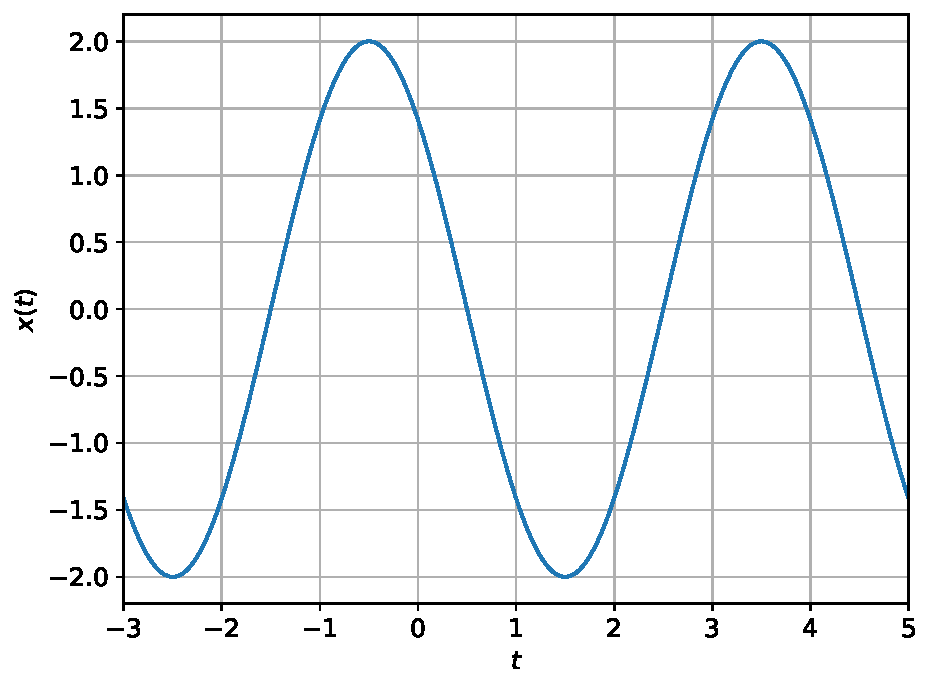
\includegraphics[scale=0.6]{figures/ctsinusoid.pdf}
\end{center}
has the functional representation
\[
x(t) = 2\cos\left(\frac{\pi}{2} (t+\tfrac{1}{2}) \right) =  2\cos\left(\frac{\pi}{2} t +\frac{\pi}{4} \right)
\]

\subsubsection{Energy of CT complex sinusoid}

Recall the energy of a CT signal $x(t)$ is    
\[
  E_x = \lim_{T\rightarrow\infty} \int\limits_{-T}^T \lvert x(t) \rvert^2 dt \; .
\]
Substituting $x(t) = e^{j\omega_0 t}$ and letting $T = N T_0$
  \[
    E_x = \lim_{N\rightarrow\infty} \int\limits_{-N T_0}^{N T_0} \underbrace{\lvert e^{j\omega_0 t} \rvert^2}_{\text{always 1}} \; dt = \lim_{N\rightarrow\infty} 2NT_0 = \infty
  \]

\subsubsection{Power of CT complex sinusoid}

Recall the power of a CT signal $x(t)$ is
\[
  E_x = \lim_{T\rightarrow\infty} \frac{1}{2T} \int\limits_{-T}^T \lvert x(t) \rvert^2 dt \; .
\]
Again, substituting $x(t) = e^{j\omega_0 t}$ and letting $T = N T_0$
\[
  E_x = \lim_{N\rightarrow\infty} \frac{1}{2NT_0} \int\limits_{-N T_0}^{N T_0} \underbrace{\lvert e^{j\omega_0 t} \rvert^2}_{\text{always 1}} \; dt = \lim_{N\rightarrow\infty} \frac{1}{2NT_0} 2NT_0 = 1
\]
  
\subsubsection{Harmonics}

Two CT complex sinusoids are {\it harmonics} of one another is both are periodic in $T_0$. This occurs when

\[
    x_k(t) = e^{jk\omega_0 t} \; \text{for} \; k = 0, \pm 1, \pm 2, \cdots
\]

The term comes from music where the vibrations of a string instrument are modeled as a weighted combination of harmonic tones. 

\subsubsection{Geometric interpretation of the Complex Exponential}

In the general case we get a sinusoid signal modulated by an exponential. Let $C = Ae^{j\phi}$ and $a = r + j\omega_0$, then
\[
  x(t) = C e^{a t} =  Ae^{j\phi} e^{(r+j\omega_0)t}
\]
Expanding the terms and using Euler's identity gives:
\[
x(t) = \underbrace{Ae^{rt}\cos(\omega_0 t+\phi)}_{\Re \text{part}} + j \underbrace{Ae^{rt}\sin(\omega_0 t+\phi)}_{\Im \text{part}}
\]
Each part is a real sinusoid whose amplitude is modulated by a real exponential.

An important visualization of the general case is to view the signal x(t) as a vector rotating counter-clockwise in the complex plane for positive $t$.

\begin{center}
 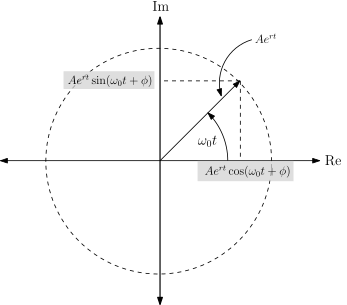
\includegraphics[scale=0.7]{figures/CT_complexsinusoid_visual}
\end{center}

For $r < 0$ the tip of the arrow traces out an inward spiral, whereas for $r > 0$ it traces out an outward spiral. For $r = 0$ it traces out the unit circle.

\newpage
\section{Discrete-time Signals}

Recall from the previous meeting that a discrete-time (DT) signal is modeled as a function $f: \mathbb{Z} \rightarrow \mathbb{C}$. We will write these as $x[n]$, $y[n]$, etc. Note $n$ is dimensionless. These are graphically plotted as stem or "lollipop" plots, as demonstrated in Fig.~\ref{fig:dtplots}.

Since the domain $\mathbb{Z}$ is usually interpreted as a time index, we will still call these {\it time-domain} signals. In the time-domain, when the co-domain is $\mathbb{R}$ we call these real DT signals. Unlike with CT signals there are no physical limitations requiring DT signals to be real, since in discrete hardware, a value at a given index can be a complex number, i.e. just a pair of numbers. However it is computationally advantageous to restrict ourselves to real arithmetic and such signals are often converted to or from CT signals, which do have to be real. For this reason real DT signals dominate in models.

\subsection{Primitive Models}

As with CT signals, we mathematically model DT signals by combining elementary/primitive functions, for example:  
\begin{itemize}
\item polynomials: $x[n] = n$, $x[n] = n^2$, etc.
\item transendental functions: $x[n] = e^n$, $x[n] = \sin(n)$, $x[n] = \cos(n)$, etc.
\item piecewise functions, e.g.
\[
x[n] = \left\{  \begin{array}{cl}
f_1[n] & n < 0\\
f_2[n] & n \geq 0\\
\end{array}\right.
\]
\end{itemize}

\begin{example}[Unit Step]
  The DT counterpart of the CT step function is the \emph{DT Unit Step}, $u[n]$:
  \[
  u[n] = \left\{  \begin{array}{cl}
    0 & n < 0\\
    1 & n \geq 0\\
  \end{array}\right.
  \]
  Note, there are not continuity issues at $n=0$ as DT functions have discrete domains.
\end{example}

\begin{example}[Sampled Pure audio tone at "middle C"]
  A \emph{sampled} signal modeling the air pressure of a specific tone, sampled at 8kHz, might be 
  \[
  x[n] = \sin\left(2\pi (261.6) \tfrac{1}{8000} n\right)
  \]
  Such DT signals are commonly used in digital music generation, storage, and playback.
\end{example}
\begin{example}[Sampled Chord]
    Similarly, the sampled chord "G", an additive mixture of tones at G, B, and D and might be modeled as
    \[
    x(t) = \sin\left(2\pi (392) \tfrac{1}{8000} n\right) + \sin\left(2\pi (494) \tfrac{1}{8000} n\right) + \sin\left(2\pi (293) \tfrac{1}{8000} n\right) 
    \]
    again sampled at 8kHz. This example shows we can use addition to build-up signals to approximate real signals of interest.
\end{example}

\subsection{Basic Transformations}

Similar to CT signals, we can also apply transformations to DT signals to increase their modeling flexibility.

\begin{itemize}
\item magnitude scaling
\[
x_2[n] = a x_1[n]
\]
for $a \in \mathbb{R}$.
\item time differences
\[
x_2[n] = x_1[n] - x_1[n-1]
\]
\item running sums
\[
x_2[n] = \sum\limits_{m = -\infty}^{n} x_1[m]
\]
\item sums
\[
y[n] = \sum\limits_{i} x_i[n]
\]
an important example we will see is the DT Fourier series.
\item multiplication (modulation)
\[
y[n] = x_1[n] x_2[n]
\]
\item time index shift
\[
x_2[n] = x_1[n+m]
\]
\begin{itemize}
\item if $m < 0$ it is called a {\it delay}
\item if $m > 0$ it is called an {\it advance}
\end{itemize}

\item time reversal
\[
x_2[n] = x_1[-n]
\]

\item decimation
\[
y[n] = x[m n]
\]
for $m \in \mathbb{Z}^+$.
\begin{itemize}
\item e.g. for $m=2$ only keep every other sample
\item e.g. for $m=3$ only keep every third sample
\item etc.
\end{itemize}

\item interpolation
\[
y[n] = \left\{  \begin{array}{cl}
x\left[ \frac{n}{m}\right] & n = 0\; , \; \pm m, , \; \pm 2m \cdots\\
0 & \mbox{else}
\end{array}\right.
\]
When $m = 2$ this inserts a zero sample between every sample of the signal.
\end{itemize}

\subsection{Characterization of Signals}

There are a few basic ways of characterizing DT signals.

\begin{definition}[Causal DT Signal]
A DT signal is \emph{causal} if $x[n] = 0$ $\forall n < 0$.
\end{definition}
\begin{definition}[Anti-Causal DT Signal]
A DT signal is \emph{anti-causal} or acausal if $x[n] = 0$ $\forall n \geq 0$.
\end{definition}

A DT signal can be written as the sum of a causal and anti-causal signal.

A DT signal is periodic if $x[n] = x[n + N] \; \forall n$ for a fixed period $N \in \mathbb{Z}$.

A DT signal is even if $x[n] = x[-n] \; \forall n$. 

A DT signal is odd if $x[n] = -x[-n] \; \forall n$.

Any DT signal can be written in terms of an even and odd component
\[
x[n] = x_e[n] + x_o[n] 
\]
where 
\[
\begin{array}{ll}
x_e[n] &= \frac{1}{2}\left\{x[n] + x[-n]\right\} \\
& \\
x_o[n] &= \frac{1}{2}\left\{x[n] - x[-n]\right\}
\end{array}
\]

Analogous to CT signals, the energy of a DT signal is
\[
E_x = \lim_{N\rightarrow\infty} \sum\limits_{-N}^N \lvert x[n]\rvert^2 \; .
\]

And the power of a DT signal is the energy averaged over an interval as that interval tends to infinity.

\[
P_x = \lim_{N\rightarrow\infty} \frac{1}{2N+1} \sum\limits_{-N}^N \lvert x[n]\rvert^2 \; .
\]

DT Signals with finite, non-zero energy and zero power are called {\it energy signals}. DT Signals with finite, non-zero power (and by implication infinite energy) are called {\it power signals}. These categories are non-exclusive, some signals are neither energy or power signals.

\subsection{DT Unit Impulse Function}

In DT the unit impulse function, denoted $\delta[n]$ is defined as
\[
\delta[n] = \left\{
\begin{array}{ll}
  1 & n = 0\\
  0 & \text{else}
\end{array}
\right.
\]
Note this definition is straightforward compared to the CT impulse as there are no continuity issues and it is not defined in terms of a distribution. It is typically draw as
\begin{center}
  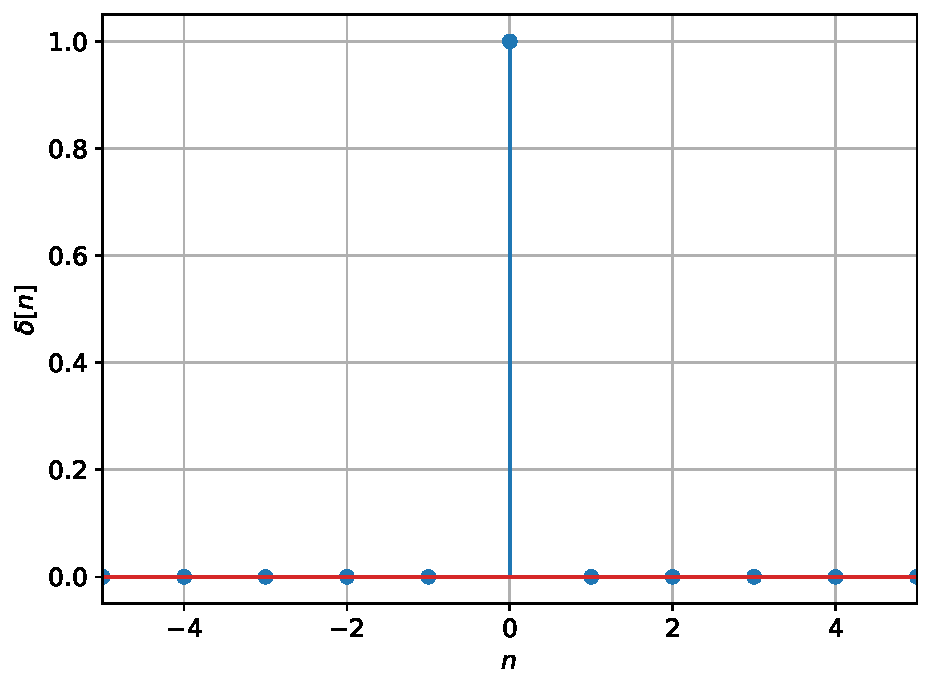
\includegraphics[scale=0.5]{figures/dtdelta.pdf}
\end{center}

Some useful properties of the DT impulse function are:

\begin{itemize}
\item Energy is 1: $\sum\limits_{n=-\infty}^{\infty} \delta[n] = 1$
\item Sampling: $x[n]\delta[n-n_0] = x[n_0]\delta[n-n_0]$
\item Sifting: $\sum\limits_{n=-\infty}^{\infty} x[n]\delta[n-n_0] = x[n_0]$
\end{itemize}

The impulse can be defined in terms of the step:
\[
\delta[n] = u[n] - u[n-1]
\]
and vice-versa
\[
u[n] = \sum\limits_{m=-\infty}^{n} \delta[m]
\]
or
\[
u[n] = \sum\limits_{k=0}^{\infty} \delta[n-k]
\]

\subsection{DT Complex Exponential}

The DT Complex Exponential is defined in a similar fashion the the CT version, but with some important differences. The general DT complex exponential is given by the expression:
\[
x[n] = Ce^{\beta n}
\]
where in general $C \in \mathbb{C}$ and $\beta \in \mathbb{C}$. It is sometimes convenient (for reasons we will see later) to write this as
\[
x[n] = C \alpha^n
\]
where $\alpha = e^{\beta}$ is a complex number $\alpha = \cos(\beta) + j\sin(\beta)$.

We now examine several special cases.

\subsubsection{DT Complex Exponential: real case}

Let $C$ and $\alpha$ be real, then there are four intervals of interest:

\begin{itemize}
\item $\alpha > 1$
\item $ 0 < \alpha < 1$
\item $-1 < \alpha < 0$
\item $\alpha < -1$
\end{itemize}

Each of these are shown in Fig.~\ref{fig:dtexpreal}.

\begin{figure}[ht]    
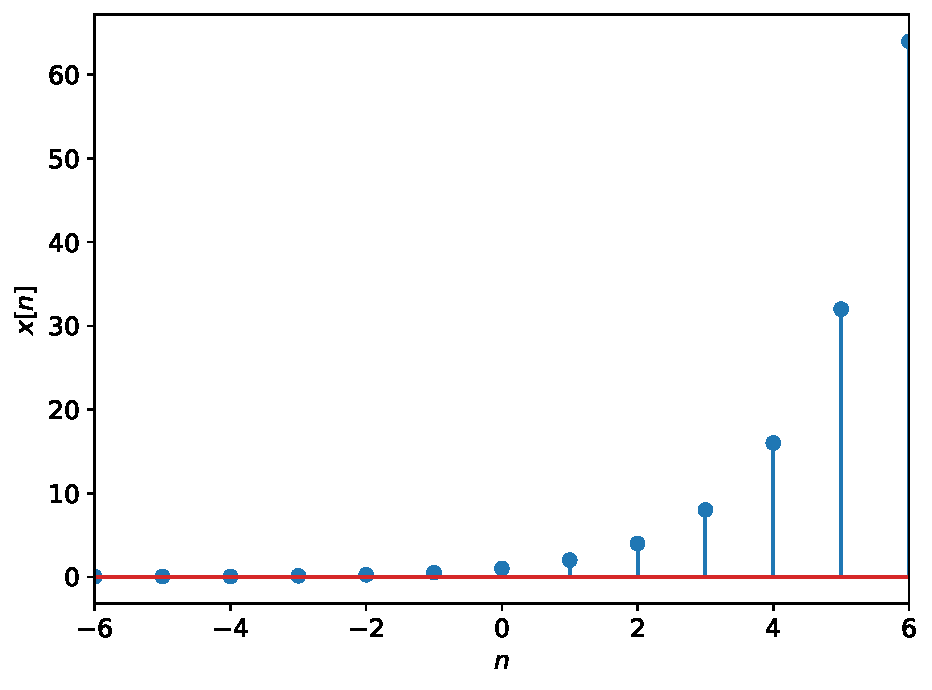
\includegraphics[scale=0.5]{figures/dtexpcase1.pdf}
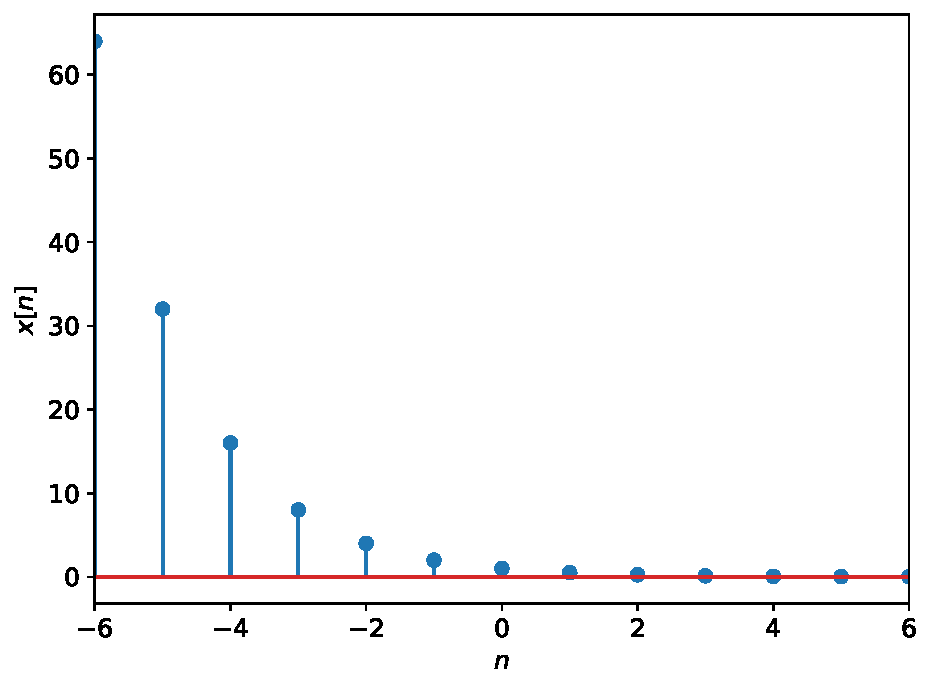
\includegraphics[scale=0.5]{figures/dtexpcase2.pdf}
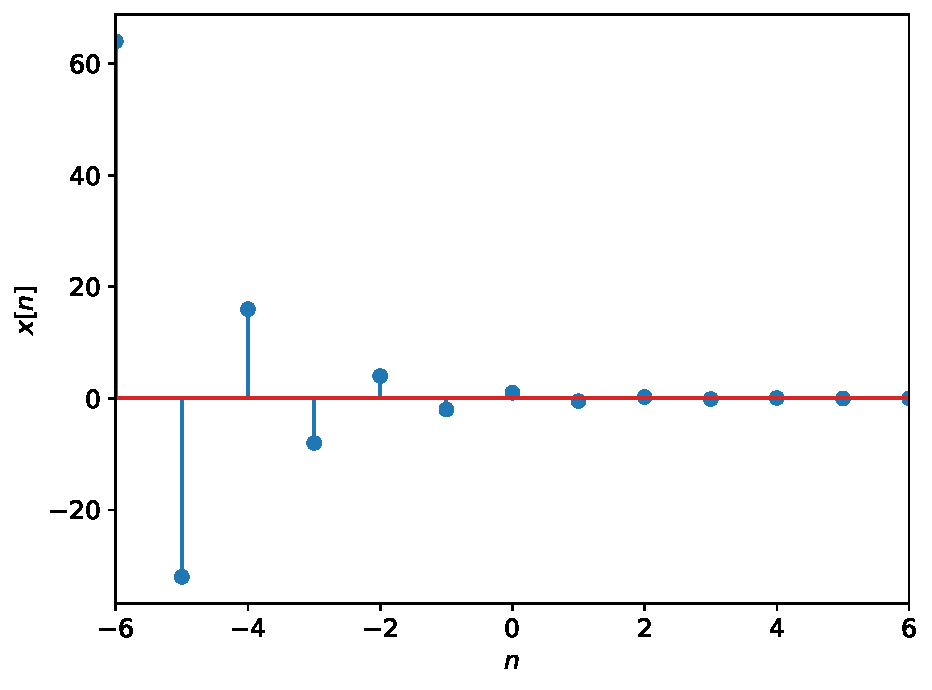
\includegraphics[scale=0.5]{figures/dtexpcase3.pdf}
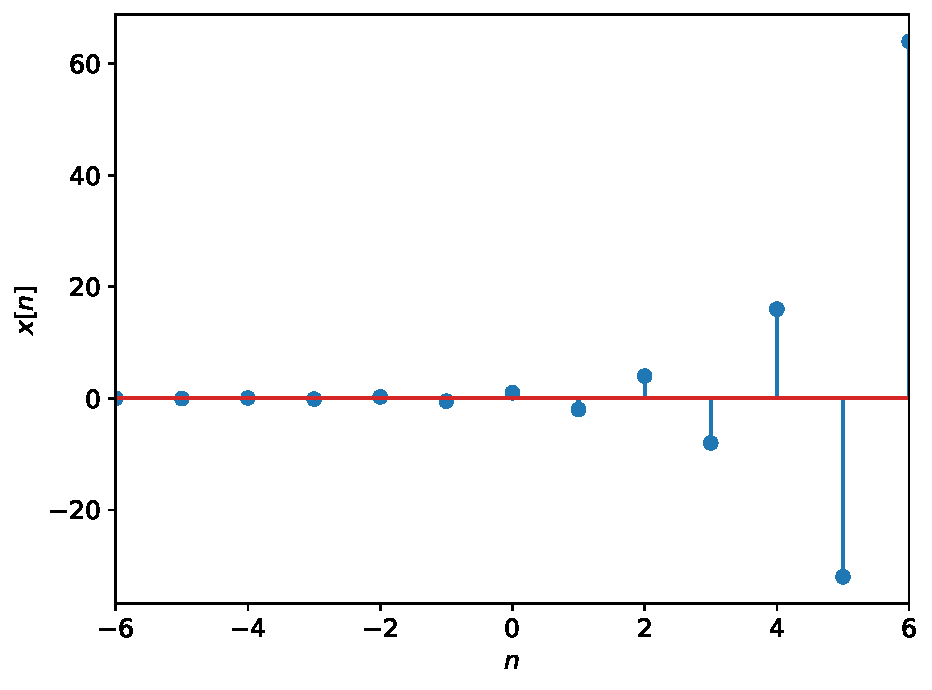
\includegraphics[scale=0.5]{figures/dtexpcase4.pdf}
\caption{ DT Complex Exponential: real case, four intervals of interest.}
\label{fig:dtexpreal}
\end{figure}

\subsubsection{DT Complex Exponential: sinusoidal case}

Let $C = 1$. When $\beta$ is purely imaginary, $\beta = j\omega_0$
\[
x[n] = e^{j\omega_0 n}
\]

As in CT, by Euler's identity:
\[
e^{j\omega_0 n} = \cos(\omega_0 n) + j\sin(\omega_0 n)
\]
and
\[
\Re(x[n]) = \cos(\omega_0 n) = \frac{1}{2}\left( e^{j\omega_0 n} + e^{-j\omega_0 n} \right)
\]
\[
\Im(x[n]) = \sin(\omega_0 n) = \frac{1}{2j}\left( e^{j\omega_0 n} - e^{-j\omega_0 n} \right)
\]

The energy and power are the same as for the CT complex sinusoid: $E_x = \infty$ and $P_x = 1$.


\subsubsection{DT Complex Exponential: sinusoidal case with phase shift}

The general DT sinusoid is

\[
x[n] = A\cos(\omega_0 n + \phi)
\]

\begin{itemize}
\item $A$ is called the amplitude
\item $\phi$ is called the phase shift
\item $\omega_0$ is now in radians (assuming $n$ is dimensionless)
\end{itemize}

\begin{center}
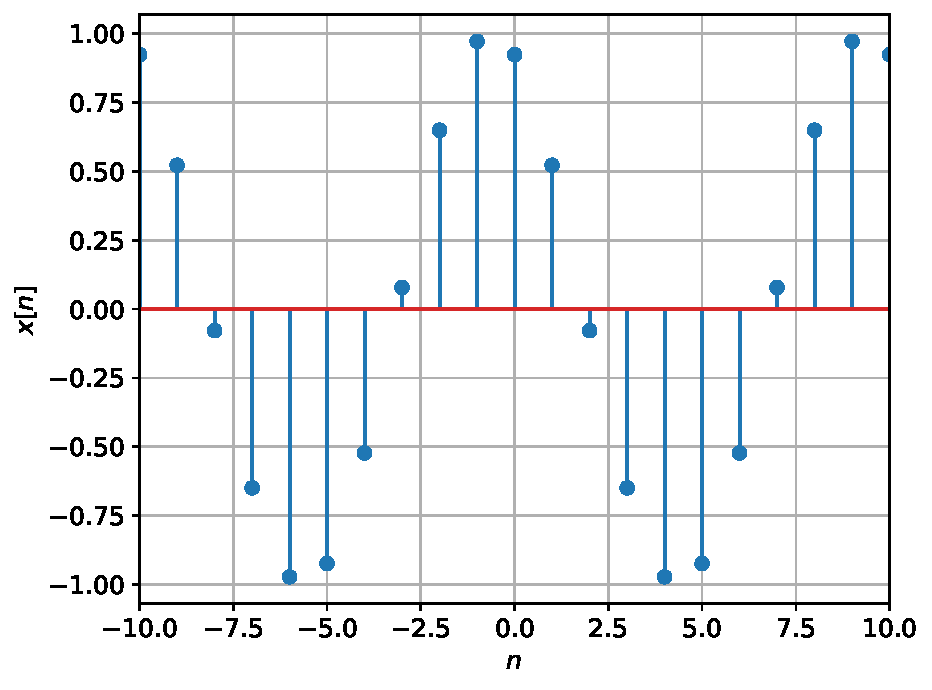
\includegraphics[scale=0.6]{figures/dtsinusoid.pdf}
\end{center}

For CT sinusoids as $\omega_0$ increases the signal oscillates faster and faster. However for DT sinusoids there is a "fastest" oscillation.

\[
e^{j\omega_0 n}\rvert_{\omega_0 = \pi} = e^{j\pi n} = (-1)^n
\]

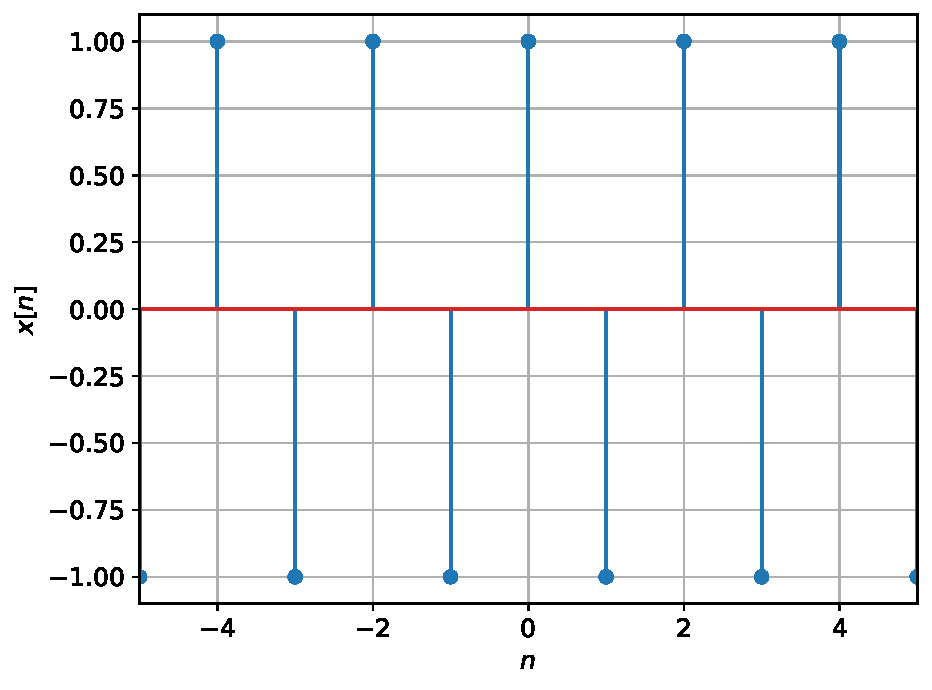
\includegraphics[scale=0.5]{figures/dtfastsin.pdf}

\subsubsection{Properties of DT complex sinusoid}

If we consider two frequencies: $\omega_0$ and $\omega_0+2\pi$. In the first case:
\[
x[n] = e^{j\omega_0 n}
\]
In the second case:
\[
\begin{array}{ll}
x[n] &= e^{j(\omega_0+2\pi) n} \\
&= \underbrace{e^{j2\pi n}}_{\text{always 1}}\; e^{j\omega_0 n} \\
&= e^{j\omega_0 n}
\end{array}
\]

Thus the two are the same signal. This has important implications later in the course.

Another difference between CT and DT complex sinusoids is periodicity. Recall for a DT signal to be periodic with period $N$
\[
x[n] = x[n+N] \; \forall n
\]
Substituting the complex sinusoid
\[
e^{j\omega_0 n} = e^{j\omega_0 (n+N)} = e^{j\omega_0 n}e^{j\omega_0 N}
\]
requires $e^{j\omega_0 N} = 1$, which implies $\omega_0 N$ is a multiple of $2\pi$:
\[
\omega_0 N = 2\pi m \;\;\; m = \pm 1, \pm 2, \cdots
\]
or equivalently
\[
\frac{|\omega_0|}{2\pi} = \frac{m}{N}
\]
thus $\omega_0$ must be a rational multiple of $\pi$. 

Two DT complex sinusoids are harmonics of one another is both are periodic in $N$,  i.e when

\[
x_k(t) = e^{jk\frac{2\pi}{N} n} \; \text{for} \; k = 0, \pm 1, \pm 2, \cdots
\]

This implies there are only $N$ distinct harmonics in DT.


\subsubsection{DT Complex Exponential: general case}

In the general case we get a sinusoid signal modulated by an exponential. Let $C = Ae^{j\phi}$ and $\beta = r + j\omega_0$, then
\[
x[n] = C e^{\beta n} =  Ae^{j\phi} e^{(r+j\omega_0)n}
\]
Expanding the terms and using Euler's identity gives:

\[
x[n] = \underbrace{Ae^{rn}\cos(\omega_0 n+\phi)}_{\Re \text{part}} + j \underbrace{Ae^{rn}\sin(\omega_0 n+\phi)}_{\Im \text{part}}
\]
Each part is a real sinusoid whose amplitude is modulated by a real exponential.

The visualization of the general case is to view the signal $x[n]$ as a vector rotating through fixed angles in the complex plane.

\begin{center}
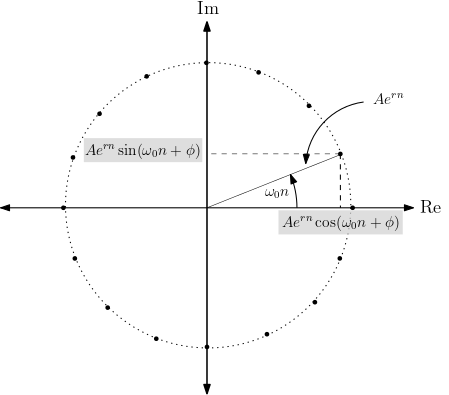
\includegraphics[scale=0.7]{figures/DT_complexsinusoid_visual}
\end{center}

\newpage
\section{CT Systems as Linear Constant Coefficient Differential Equations}

Recall a system is a transformation of signals, turning the input signal into the output signal. While this might seem like a new concept to you, you already know something about them from your differential equations course, i.e. MATH 2214 and your circuits course.

For example, consider the following circuit:
\begin{center}
  \begin{circuitikz}[american voltages,scale=0.8, every node/.style={transform shape}]
    \draw
    (0,2.3) to[battery, l=$1\mbox{ VDC}$] (0,0)
    (3,2) node[spdt,xscale=-1,yscale=-1,anchor=in] (Sw) {}
    (0,2.3) to[short] (Sw.out 2)
    (Sw.out 1) to[short] (1.8,0)
    (0,0) to[short, -o] (8,0)
    (3,2) to[short] (4,2)
    (4,2) to[open, v=$x(t)$] (4,0)
    (4,2) to[R, l=$R$] (6,2)
    (6,2) to[short, -o] (8,2)
    (6,0) to[C, l=$C$] (6,2)
    (8,2) to[open, v=$V_C(t)$] (8,0);
  \end{circuitikz}
\end{center}
where the switch moves position at $t = 0$. The governing equation for the circuit when $t < 0$ is
\[
\frac{dV_c}{dt}(t) + \frac{1}{RC}V_c(t) = 0
\]
a \emph{homogeneous} differential equation of first-order. From a DC analysis, the initial condition on the capacitor voltage is $V_C(0^-) = 0$, so there is no current flowing prior to $t = 0$ and the solution is $V_C(t) = 0$ for $t < 0$.

After the switch is thrown, the governing equation for the circuit when $t \geq 0$ is
\[
\frac{dV_c}{dt}(t) + \frac{1}{RC}V_c(t) = \frac{1}{RC}
\]
Since the voltage across the capacitor cannot change instantaneously $V_C(0^-) = V_C(0^+) = 0$, giving the auxillary condition necessary to solve this equation, which has the form
\[
V_C(t) = A + Be^{-\frac{1}{RC}t}
\]
Using the auxillary condition we find
\[
V_C(0) = A + Be^{-\frac{1}{RC}0} = A + B = 0 \mbox{ which implies } B = -A 
\]
Subsitution back into the differential equation and equating the coefficients gives $A = 1$. Thus the voltage for $t \geq 0$ is
\[
V_C(t) = 1 - e^{-\frac{1}{RC}t}
\]

Suppose we consider the voltage after the switch as the input signal $x(t)$ to the system composed of the series RC. As we have seen previously a mathematical model of the switch is the unit step $x(t) = u(t)$. Suppose we consider the capacitor voltage at the outut of the system, so that $y(t) = V_C(t)$. Then we can consider the system to be represented by the \emph{linear, constant-coefficient differential equation}
\[
\frac{dy}{dt}(t) + \frac{1}{RC}y(t) = \frac{1}{RC}x(t)
\]
where $x(t) = u(t)$ and the solution $y(t)$ is the \emph{step response}
\[
y(t) = \left(1 - e^{-\frac{1}{RC}t}\right)u(t)
\]

As we will see later this representation of systems is central to the course, so we take some time here to review the solution of such equations.
 
\subsection{Solving Linear, Constant Coefficient Differential Equations}

NOTE THIS SUBSECTION MOVED TO PREREQUISITES

A linear, constant coefficient (LCC) differential equation is of the form
\[
a_0\, y + a_1\, \frac{dy}{dt} + a_2\, \frac{d^2y}{dt^2} + \cdots + a_N\, \frac{d^Ny}{dt^N}  = b_0\, x + b_1\, \frac{dx}{dt} + bb_2\, \frac{d^2x}{dt^2} + \cdots + b_M\, \frac{d^My}{dt^M}
\]
which can be written compactly as
\[
\sum\limits_{k = 0}^{N} a_k\, \frac{d^ky}{dt^k} = \sum\limits_{k = 0}^{M} b_k\, \frac{d^kx}{dt^k}
\]

It is helpful to clean up this notation using the derivative operator $D^n = \frac{d^n}{dt^n}$. For example
$D^2y = \frac{d^2y}{dt^2}$ and $D^0 y= y$. To give for form as
\[
\sum\limits_{k = 0}^{N} a_k\, D^k y = \sum\limits_{k = 0}^{M} b_k\, D^k x
\]

We can factor out the derivative operators
\[
a_0y + a_1Dy + a_2D^2y + \cdots + a_ND^Ny  = b_0\, x + b_1\, Dx + b_2\, D^2x + \cdots + b_M\, D^M x
\]
\[
\underbrace{\left(a_0 + a_1D + a_2D^2 + \cdots + a_ND^N\right)}_{\text{Polynimial in } D, Q(D)} y = \underbrace{\left(b_0 + b_1 D + b_2 D^2 + \cdots + b_M D^M\right)}_{\text{Polynimial in } D, P(D)} x
\]
to give:
  
\[
Q(D)y = P(D)x
\]
You learned how to solve these in differential equations (Math 2214) as
\[
y(t) = y_\text{h}(t) + y_\text{p}(t)
\]

The term $y_\text{h}(t)$ is the solution of the homogeneous equation
\[
Q(D)y = 0
\]
Given the $N-1$ auxillary conditions $y(t_0) = y_0$, $Dy(t_0) = y_1$, $D^2y(t_0) = y_2$, up to $D^{N-1}y(t_0) = y_{N-1}$.

The term $y_\text{p}(t)$ is the solution of the particular equation
\[
Q(D)y = P(D)x
\]
for a given $x(t)$.

Rather than recapitulate the solution to $y_\text{h}(t)$ and $y_\text{p}(t)$ in the general case we focus on the homogeneous solution $y_\text{h}(t)$ only. The reason is that we will use the homogeneous solution to find the impulse response below and take a different approach to solving the general case for an arbitrary input using the impulse response and convolution (next week).

To solve the homogenous system:

\textbf{Step 1:} Find the \emph{characteristic equation} by replacing the derivative operators by powers of an aribrary complex variable $s$.
\[
Q(D) = a_0 + a_1D + a_2D^2 + \cdots + a_ND^N
\]
becomes
\[
Q(s) = a_0 + a_1s + a_2s^2 + \cdots + a_Ns^N
\]
a polynomial in $s$ with $N$ roots $s_i$ for $i = 1, 2, \cdots, N$ such that
\[
(s - s_1)(s-s_2)\cdots(s-s_N) = 0
\]

\textbf{Step 2:} Select the form of the solution, a sum of terms corresponding to the roots of the characteristic equation.

\begin{itemize}
\item For a real root $s_1\in \mathbb{R}$ the term is of the form
  \[
  C_1 e^{s_1 t}.
  \]
\item For a pair of complex roots (they will always be in pairs) $s_{1,2} = a \pm jb$ the term is of the form
  \[
  C_1 e^{s_1 t} + C_2 e^{s_2 t} = e^{a t}\left(C_3\cos(bt) + C_4\sin(bt)\right) = C_5 e^{a t}\cos(bt + C_6).
  \]
\item For a repeated roots $s_1$, repeated r times, the term is of the form
  \[
  e^{s_1 t} (C_0 + C_1 t + \cdots + C_{r-1} t^{r-1}).\]
\end{itemize}

\textbf{Step 3:} Solve for the unknown constants in the solution using the auxillary conditions. 

We now examine two common special cases, when $N=1$ (first-order) and when $N=2$ (second-order).

\subsubsection{First-Order Homogeneous LCCDE}

Consider the first order homogeneous differential equation
\[
\frac{dy}{dt}(t) + ay(t) = 0 \mbox{ for } a \in \mathbb{R}
\]
The characteristic equation is given by
\[
s + a = 0
\]
which has a single root $s_1 = -a$. The solution is of the form
\[
y(t) = Ce^{s_1 t} = Ce^{-a t} 
\]
where the constant $C$ is found using the auxillary condition $y(t_0) = y_0$.

\textit{Example}: Consider the homogeneous equation
\[
\frac{dy}{dt}(t) + 3y(t) = 0 \mbox{ where } y(0) = 10
\]
The solution is
\[
y(t) = Ce^{-3 t} 
\]
To find $C$ we use the auxillary condition
\[
y(0) = Ce^{-3 \cdot 0} = C = 10
\]
and the final solution is
\[
y(t) = 10e^{-3 t} 
\]
\subsubsection{Second-Order Homogeneous LCCDE}

Consider the second-order homogeneous differential equation
\[
\frac{d^2y}{dt^2}(t) + a\frac{dy}{dt}(t) + by(t) = 0 \mbox{ for } a,b \in \mathbb{R}
\]
The characteristic equation is given by
\[
s^2 + as + b = 0
\]

Let's look at several examples to illustrate the functional forms.

Example 1:
\[
\frac{d^2y}{dt^2}(t) + 7\frac{dy}{dt}(t) + 10y(t) = 0 
\]
The characteristic equation is given by
\[
s^2 + 7s + 10 = 0
\]
which has roots $s_1 = -2$ and $s_2 = -5$. Thus the form of the solution is
\[
y(t) = C_1e^{-2t} + C_2e^{-5t}
\]

Example 2:
\[
\frac{d^2y}{dt^2}(t) + 2\frac{dy}{dt}(t) + 5y(t) = 0 
\]
The characteristic equation is given by
\[
s^2 + 2s + 5 = 0
\]
which has complex roots $s_1 = -1+j2$ and $s_1 = -1-j2$. Thus the form of the solution is
\[
y(t) = e^{-t}\left(C_1\cos(2t) + C_2\sin(2t)\right)
\]

Example 3:
\[
\frac{d^2y}{dt^2}(t) + 2\frac{dy}{dt}(t) + y(t) = 0 
\]
The characteristic equation is given by
\[
s^2 + 2s + 1 = 0
\]
which has a root $s_1 = -1$ repeated $r=2$ times. Thus the form of the solution is
\[
y(t) = e^{-t}\left(C_1 + C_2t\right)
\]

In each of the above cases the constants, $C_1$ and $C_2$, are found using the auxillary conditions $y(t_0)$ and $y\prime(t_0)$.

\subsection{Finding the impulse response of a system described by a LCCDE}

As we will see next week an important response of a system is the one that corresponds to an impulse input, i.e. the \emph{impulse response} $y(t) = h(t)$ when $x(t) = \delta(t)$. Thus we focus here on a recipe for solving LCCDEs for this special case when $M \leq N$. We will skip the derivation of why this works.

Our goal is to find the solution to $Q(D)y = P(D)x$ when $x(t)=\delta(t)$.

\textbf{Step 1:} Let $y_h(t)$ be the homogeneous solution to $Q(D)y_h = 0$ for auxillary conditions
  \[
    D^{N-1}y_h(0^+) = 1 \; , \; D^{N-2}y_h(0^+) = 0 \; , \; \text{etc.} \; y_h(0^+) = 0 
    \]
    
\textbf{Step 2:} Assume a form for $h(t)$ given by:
  \[
  h(t) = \underbrace{b_N\delta(t)}_{=0 \text{ unless } N=M} + \underbrace{\left[ P(D)y_h\right]}_{\text{apply } P(D) \text{ to } y_n(t)}u(t)
  \]

Recall from above the homogeneous solution depends on the roots of the characteristic equation $Q(D) = 0$.

\begin{itemize}
\item roots are either real, or
\item roots occur in complex conjugate pairs, or
\item repeated roots.
\end{itemize}

Example 1: Find the impulse response of the LCCDE
\[
\frac{dy}{dt}(t) + y(t) = x(t)
\]
The characteristic equation is given by
\[
s + 1 = 0
\]
which has a single root $s_1 = -1$. The solution is of the form
\[
y_h(t) = Ce^{-t} 
\]
with the special auxillary condition $y(0) = 1$, so that
\[
y_h(t) = e^{-t} 
\]
Since $P(D) = 1$ and $N = 1 \neq M = 0$ the impulse response is
\[
h(t) = \underbrace{b_N\delta(t)}_{=0} + \left[ \underbrace{P(D)}_{1}y_h(t)\right]u(t) = e^{-t}u(t)
\]

Example 2: Find the impulse response of the LCCDE
\[
\frac{dy}{dt}(t) + y(t) = \frac{dx}{dt}(t) + x(t)
\]
The homogeneous solution is the same as in Example 1,
\[
y_h(t) = e^{-t} 
\]
however now $M = N = 1$ with $b_1 = 1$ and $P(D) = D+1$. Thus, the impulse response is
\[
h(t) = \underbrace{b_N}_{=1}\delta(t) + \left[ \underbrace{P(D)}_{D+1}y_h(t)\right]u(t) = \delta(t) + \left\{[D+1]e^{-t}\right\}u(t) = \delta(t) + [- e^{-t} + e^{-t}]u(t) = \delta(t) 
\]

Example 3: Find the impulse response of the LCCDE
\[
\frac{d^2y}{dt^2}(t) + 7\frac{dy}{dt}y(t) + 10y(t) = x(t) 
\]
The characteristic equation is given by
\[
s^2 + 7s + 10 = 0
\]
which has roots $s_1 = -2$ and $s_2 = -5$. Thus the form of the solution is
\[
y_h(t) = C_1e^{-2t} + C_2e^{-5t}
\]
The special auxillary conditions are $y_h(0) = 0$ and $y^\prime_h(0) = 1$. Using these conditions
\[
y_h(0) = C_1e^{-2t} + C_2e^{-5t} |_{t = 0} = C_1 + C_2 = 0
\]
\[
y^\prime_h(0) = -2C_1e^{-2t} - 5C_2e^{-5t} |_{t = 0} = -2C_1 -5C_2 = 1
\]
Solving for the constants gives $C_1 = \frac{1}{3}$ and $C_2 = -\frac{1}{3}$. Since $P(D) = 1$ and $N = 2 \neq M = 0$ the impulse response is
\[
h(t) = \underbrace{b_N\delta(t)}_{=0} + \left[ \underbrace{P(D)}_{1}y_h(t)\right]u(t) = \frac{1}{3} e^{-2t}u(t) - \frac{1}{3} e^{-5t}u(t)
\]


\newpage
\section{DT systems as linear constant coefficient difference equations}

A \emph{difference equation} is a relation among combinations of two DT functions and shifted versions of them. Similar to differential equations where the solution is a CT function, the solution to a difference equation is a DT function. For example:
\[                         
y[n+1] + \frac{1}{2}y[n] = x[n] 
\]
is a first order, linear, constant-coefficient difference equation. Given $x[n]$ the solution is a function $y[n]$. We can view this as a representation of a DT system, where $x[n]$ is the input signal and $y[n]$ is the output.

There is a parallel theory to differential equations for solving difference equations. However in this lecture we will focus specifically on the iterative solution of linear, constant-coefficient difference equations and the case when the input is a delta function, as this is all we need for this course.

\subsection{Definition of linear constant coefficient difference equation}

A \emph{linear}, \emph{constant-coefficient}, difference equation (LCCDE) comes in one of two forms.

\begin{itemize}
  \item Delay form. 
  \[    
  \sum\limits_{k = 0}^N a_k y[n-k] = \sum\limits_{k = 0}^M b_k x[n-k]
  \]
  or
  \[
  a_0y[n] + a_1y[n-1] + \cdots a_N y[n-N] = b_0 x[n] + \cdots b_Mx[n-M]
  \]
  
\item Advance form. Let $n\rightarrow n+N$, then the delay form becomes
  \[    
  \sum\limits_{k = 0}^N a_k y[n+N-k] = \sum\limits_{k = 0}^M b_k x[n+N-k]
  \]
  or 
  \[
  a_0y[n+N] + a_1y[n+N-1] + \cdots a_N y[n] = b_0 x[n+N] + \cdots b_Mx[n+N-M]
  \]
\end{itemize}

The {\it order} of the system is given by $N$. The delay and advance forms are equivalent because the equation holds for any $n$, and we can move back and forth between them as needed by a constant index-shift.

\begin{example}[$N=2$, $M=1$]
  The delay form is
  \[
  a_0y[n] + a_1 y[n-1] + a_2 y[n-2] = b_0 x[n] + b_1 x[n-1]
  \]
  Replacing $n \rightarrow n+2$, the advance form is
  \[
  a_0 y[n+2] + a_1 y[n+1] + a_2 y[n] = b+0 x[n+2] + b_1 x[n+1]
  \]
  $\blacksquare$
\end{example}

It will be convenient to define the operator $E^m$ as shifting a DT function by positive $m$, i.e. $E^m x[n] = x[n+m]$, and the operator $D^m$ as shifting a DT function by negative $m$, i.e. $D^m x[n] = x[n-m]$. These are called the advance and delay operators respectively. Then, the advance form of the difference equation using this operator notation is
\[
a_0y[n+N] + a_1y[n+N-1] + \cdots a_N y[n] = b_0 x[n+N] + \cdots b_Mx[n+N-M]
\]
\[
a_0 E^Ny + a_1E^{N-1}y + \cdots a_N y = b_0 E^{N}x + \cdots b_M E^{N-M}x
\]
Factoring out the advance operators gives
\[
\underbrace{\left(a_0E^N + a_1E^{N-1} + \cdots a_N\right)}_{Q(E)} y = \underbrace{\left(b_M E^{N} + \cdots b_M E^{N-M}\right)}_{P(E)} x
\]
or
\[
Q(E)y[n] = P(E)x[n]
\]

Similarly, the delay form of the difference equation using this operator notation is
\[
a_0y[n] + a_1y[n-1] + \cdots a_N y[n-N] = b_0 x[n] + \cdots b_Mx[n-M]
\]
\[
a_0y[n] + a_1 Dy + \cdots a_N D^N y = b_0 x + \cdots b_MD^M x
\]
Note: The DT delay operator $D$ is similar, but \emph{not} identical to the derivative operator $D$ in CT.

\begin{example}
  Consider the difference equation
  \[
  2y[n+1] + 5y[n] + 2y[n-1] = 2x[n+1]
  \]
  The advance form would be:
  \[
  2y[n+2] + 5y[n+1] + 2y[n] = 2x[n+2]
  \]
  or using the advance operator
  \[
  \left(2E^2 + 5E + 2\right)y = 2E^2x
  \]
  with $Q(E) = 2E^2 + 5E + 2$ and $P(E) = 2E^2$.\\[1em]
  The delay form would be:
  \[
  2y[n] + 5y[n-1] + 2y[n-2] = 2x[n]
  \]
  or using the delay operator
  \[
  \left(2D^2 + 5D + 2\right)y = 2x
  \]
$\blacksquare$
\end{example}

\subsection{Iterative solution of LCCDEs}

Difference equations are different (pun!) from differential equations in that they can be solved by manually running the equation forward using previous values of the output and current and previous values of the input, given some initial conditions. This is called an \emph{iterative} solution for this reason.

To perform an iterative solution we need the difference equation in delay form
\[
a_0y[n] + a_1y[n-1] + \cdots a_N y[n-N] = b_0 x[n] + \cdots b_Mx[n-M]
\]
We then solve for the current output $y[n]$
\[
y[n] =  - \left(\frac{a_1}{a_0}y[n-1] + \cdots \frac{a_N}{a_0} y[n-N]\right) + \frac{b_0}{a_0} x[n] + \cdots \frac{b_M}{a_0}x[n-M]
\]

Now lets examine what this expression says in words. To compute the current output $y[n]$ we need the value of the \emph{previous} $N-1$ outputs, the value of the \emph{current} input $x[n]$ and $M-1$ \emph{previous} inputs (and the coefficients). Then we can compute the next output $y[n+1]$ by adding the previous computation result for $y[n]$ to our list of things to remember, and forgetting one previous value of $y$. This can continue as long as we like.

\begin{example}
  Consider the first-order difference equation
  \[
  y[n+1] + y[n] = x[n+1]
  \]
  where $y[-1] = 1$ and $x[n] = u[n]$. We first convert this to delay form
  \[
  y[n] = -y[n-1] + x[n]\; .
  \]
  Then we can compute $y[0]$ as
  \[
  y[0] = -y[-1] + x[0] = -1 + 1 = 0
  \]
  and continuing
  \begin{align*}
  y[1] &= -y[0] + x[1] = 0 + 1 = 1\\
  y[2] &= -y[1] + x[2] = -1 + 1 = 0\\
  y[3] &= -y[2] + x[3] = 0 + 1 = 1\\
  \mbox{etc.}
  \end{align*}
  We can see that this will continue to give the alternating sequence $1,0,1,0,1,\cdots$.
$\blacksquare$
\end{example}

\subsection{Solution of the homogeneous LCCDE}

Note the iterative solution does not give us (directly) and analytical expression for the output at arbitrary $n$. We have to start at the initial conditions and compute our way up to $n$. We now consider an analytical solution when the input is zero, the solution to the \emph{homogeneous} difference equation
\[
Q(E)\, y = a_0y[n+N] + a_1y[n+N-1] + \cdots a_N y[n] = 0 \; .
\]
given $N$ sequential auxiliary conditions on $y$.

Similar to differential equations, the homogeneous solution depends on the roots of the characteristic equation $Q(E)=0$ whose roots are either real or occur in complex conjugate pairs. Let $\lambda_i$ be the i-th root of $Q(E) = 0$, then the solution is of the form
\[
y[n] = \sum\limits_{i=1}^N C_i \lambda_i^{n}
\]
where the parameters $C_i$ are determined from the auxiliary conditions.

For a real system (when the coefficients of the difference equation are real) and when the roots are complex $\lambda_{1,2} = |\lambda|e^{\pm j\beta}$, it is cleaner to assume a form for those terms as
\[
y[n] = C |\lambda|^n\cos(\beta n + \theta)
\]
for constants $C$ and $\theta$.

\begin{example}[First-Order]
  Find the solution to the first-order homogeneous LCCDE
  \[
  y[n+1] + \frac{1}{2}y[n] = 0 \mbox{ with } y[0] = 5 \; .
  \]
  Note $Q(E) = E + \frac{1}{2}$ has a single root $\lambda_1 = -\frac{1}{2}$. Thus the solution is of the form
  \[
  y[n] = C\left( -\frac{1}{2}\right)^n
  \]
  where the parameter $C$ is found using
  \[
  y[0] = C = 5
  \]
  to give the final solution
  \[
  y[n] = 5\left( -\frac{1}{2}\right)^n
  \]
  $\blacksquare$  
\end{example}

\begin{example}[Second-Order, Complex Roots]
  Find the solution to the second-order homogeneous LCCDE
  \[
  y[n+2] + y[n+1] + \frac{1}{2}y[n] = 0 \mbox{ with } y[0] = 1 \mbox{ and } y[1] = 0\; .
  \]
  Note $Q(E) = E^2 + E + \frac{1}{2}$ has a pair of complex roots $\lambda_{1,2} = -\frac{1}{2} \pm j\frac{1}{2}$. Thus the solution is of the form
  \[
  y[n] = C \left|\frac{1}{\sqrt{2}}\right|^n\cos\left(\frac{\pi}{4} n + \theta\right)
  \]
  where the parameters are found using
  \[
  y[0] = C\cos\left(\theta\right) = 1
  \]
  \[
  y[1] = C\frac{1}{\sqrt{2}}\cos\left(\frac{\pi}{4} + \theta\right) = 0
  \]
  This is true when
  \[
  C = \sqrt{2} \mbox{ and } \theta = \frac{\pi}{4} + 2\pi m
  \]
  or
  \[      
  C = -\sqrt{2} \mbox{ and } \theta = -\frac{3\pi}{4} + 2\pi m
  \]
  for any $m\in \mathbb{Z}$ since $\cos$ is periodic in $2\pi$. A final solution is then
  \[
  y[n] = \sqrt{2} \left|\frac{1}{\sqrt{2}}\right|^n\cos\left(\frac{\pi}{4} n + \frac{\pi}{4}\right)
  \]
  $\blacksquare$
\end{example}

\subsection{Impulse response from LCCDE}

Today our goal is to find the solution to $Q(E)y=P(E)x$ when $x[n] = \delta[n]$ assuming $y[n] = 0$ for $n < 0$, giving the \emph{impulse response} $y[n] = h[n]$. We skip the derivation here and just give a procedure.

\textbf{Step 1:} Let $y_h$ be the homogeneous solution to $Q(E)y_h=0$ for $n > N$.

\textbf{Step 2:} Assume a form for $h[n]$ given by
\[
h[n] = \frac{b_N}{a_N}\delta[n] + y_h[n]u[n]
\]

\textbf{Step 3:} Using the iterative procedure above find the $N$ auxiliary conditions we need by,

\begin{itemize}
\item first, rewrite the equation in delay form and solving for $y[n]$,
\item then let $x[n] = \delta[n]$ and manually compute $h[0]$ assuming $h[n] = 0$ for $n < 0$,
\item repeating the previous step for $h[1]$, continuing up to $h[N-1]$.
\end{itemize}

\textbf{Step 4:} Using the auxillary conditions in step 3, solve for the constants in the solution $h[n]$ from step 2.

\begin{example}

  Find the impulse response of the system given by
  \[
  y[n+2] -\frac{1}{4}y[n+1] -\frac{1}{8}y[n]= 2x[n+1]
  \]

  For step 1 we solve the equation
  \[
  y_h[n+2] -\frac{1}{4}y_h[n+1] -\frac{1}{8}y_h[n] = 0
  \]
  which is of the form
  \[
  y_h[n] = C_1 \left( -\frac{1}{4}\right)^n + C_2 \left( \frac{1}{2}\right)^n
  \]
  since the roots of $Q(E) = E^2 - \frac{1}{4}E - \frac{1}{8}$ are $-\frac{1}{4}$ and $\frac{1}{2}$.

  For step 3, we find the auxiliary conditions needed to find $C_1$ and $C_2$ by rewriting the original equation in delay form and solving for $y[0]$ and $y[1]$ when $x[n] = \delta[n]$.
  \[
  y[n] = \frac{1}{4}y[n-1] + \frac{1}{8}y[n-2] + 2x[n-1]
  \]    
  Let $x[n] = \delta[n]$ and manually compute $y[0]$ assuming $y[n] = 0$ for $n < 0$
  \[
  y[0] = \frac{1}{4}\underbrace{y[0-1]}_{0} + \frac{1}{8}\underbrace{y[0-2]}_{0} + 2\underbrace{\delta[0-1]}_{0} = 0
  \]
  Repeat for $y[1]$
  \[
  y[1] = \frac{1}{4}\underbrace{y[1-1]}_{0} + \frac{1}{8}\underbrace{y[1-2]}_{0} + 2\underbrace{\delta[1-1]}_{1} = 2
  \]  
  Now we find the constants using step 4
  \[
  h[0] = C_1  + C_2  = 0
  \]
  \[
  h[1] = C_1 \left( -\frac{1}{4}\right) + C_2 \left( \frac{1}{2}\right) = 2
  \]
  which gives $C_1 = -\frac{8}{3}$ and $C_2 = \frac{8}{3}$. Thus the final impulse response is
  \[
  h[n] = \frac{b_N}{a_N}\delta[n] + y_h[n]u[n] = -\frac{8}{3}\left( -\frac{1}{4}\right)^nu[n] + \frac{8}{3}\left( \frac{1}{2}\right)^n u[n]
  \]
  since $b_N = 0$.
$\blacksquare$
\end{example}

  Note we can confirm our closed-form result in the previous example, for a few values of $n$, by iteratively solving the difference equation
  \[
    h[0] = \frac{1}{4}\underbrace{h[0-1]}_{0} + \frac{1}{8}\underbrace{h[0-2]}_{0} + 2\underbrace{\delta[0-1]}_{0} = 0
  \]
  \[
      h[1] = \frac{1}{4}\underbrace{h[1-1]}_{0} + \frac{1}{8}\underbrace{h[1-2]}_{0} + 2\underbrace{\delta[1-1]}_{1} = 2
    \]
    \[
      h[2] = \frac{1}{4}\underbrace{h[2-1]}_{2} + \frac{1}{8}\underbrace{h[2-2]}_{0} + 2\underbrace{\delta[2-1]}_{0} = \frac{1}{2}
    \]
    \[
      h[3] = \frac{1}{4}\underbrace{h[3-1]}_{\frac{1}{2}} + \frac{1}{8}\underbrace{h[3-2]}_{2} + 2\underbrace{\delta[2-1]}_{0} = \frac{3}{8}
    \]
    and comparing to our closed-form solution a the same values of $n$
    \[
    h[0] = -\frac{8}{3} + \frac{8}{3} = 0
    \]
    \[
    h[1] = -\frac{8}{3}\left( -\frac{1}{4}\right) + \frac{8}{3}\left( \frac{1}{2}\right) = 2
    \]
    \[
    h[2] = -\frac{8}{3}\left( -\frac{1}{4}\right)^2 + \frac{8}{3}\left( \frac{1}{2}\right)^2 = \frac{1}{2}
    \]
    \[
    h[3] = -\frac{8}{3}\left( -\frac{1}{4}\right)^3 + \frac{8}{3}\left( \frac{1}{2}\right)^3 = \frac{3}{8}
    \]

\begin{example}
  Find the impulse response of the system given by
  \[
  y[n+1] - \frac{1}{2}y[n] = x[n+1] + x[n]
  \]

  In step 1 we note the solution to $Q(E)y[n] = 0$ is of the form
  \[
  y_h[n] = C\left( \frac{1}{2}\right)^n
  \]
  From step 2 we note $b_N = 1$ and $a_N = -\frac{1}{2}$, so that
  \[
  h[n] = -2\delta[n]  +  C\left( \frac{1}{2}\right)^n\, u[n]
  \]
  In step 3 we manually find $h[0]$
  \begin{align*}
    y[n] &= \frac{1}{2}y[n-1] + x[n] + x[n-1]\\
    h[n] &= \frac{1}{2}y[n-1] + \delta[n] + \delta[n-1]\\
    h[0] &= 0 + 1 + 0 = 1
  \end{align*}
  And in step 4 we solve for $C$
  \[
  h[0] = -2  +  C = 1 \mbox{ implies } C = 3
  \]
  to give
  \[
  h[n] = -2\delta[n]  +  3\left( \frac{1}{2}\right)^n\, u[n]
  \]
  $\blacksquare$
\end{example}


\newpage
\chapter{Linear time invariant CT systems}

\section{System types}

A system is an interconncted set of components or sub-systems. Mathematically a system is a transformation between one or more signals, a rule that maps functions to functions.

\begin{itemize}
\item single input - single output (SISO) system.
  \begin{center}
    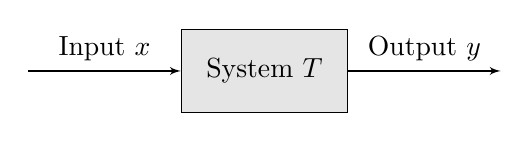
\begin{tikzpicture}[auto, node distance=3cm,>=latex']
      \node [input, name=input] {};
      \node [block, right of=input] (system) {System $T$};
      \node [output, right of=system] (output) {};
      
      \draw [draw,->] (input) -- node {Input $x$} (system);
      \draw [->] (system) -- node {Output $y$} (output);
    \end{tikzpicture}
  \end{center}
\item single input - multiple output (SIMO) system
  \begin{center}
    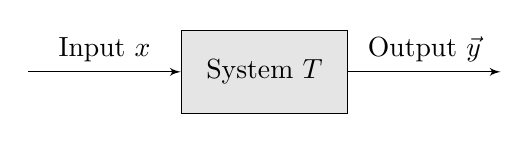
\begin{tikzpicture}[auto, node distance=3cm,>=latex']
      \node [input, name=input] {};
      \node [block, right of=input] (system) {System $T$};
      \node [output, right of=system] (output) {};
      
      \draw [draw,->] (input) -- node {Input $x$} (system);
      \draw [->] (system) -- node {Output $\vec y$} (output);
    \end{tikzpicture}
  \end{center}
\item general case, multiple input - multiple output (MIMO)
  \begin{center}
    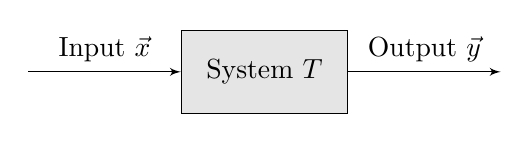
\begin{tikzpicture}[auto, node distance=3cm,>=latex']
      \node [input, name=input] {};
      \node [block, right of=input] (system) {System $T$};
      \node [output, right of=system] (output) {};
      
      \draw [draw,->] (input) -- node {Input $\vec x$} (system);
      \draw [->] (system) -- node {Output $\vec y$} (output);
    \end{tikzpicture}
  \end{center}
\end{itemize}

We will focus on single input - single output, CT and DT systems.

\begin{itemize}
\item If both input and output are CT signals, it is a CT system.
  \begin{center}
    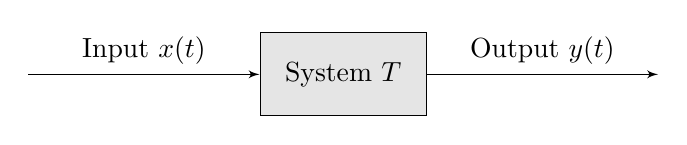
\begin{tikzpicture}[auto, node distance=4cm,>=latex']
      \node [input, name=input] {};
      \node [block, right of=input] (system) {System $T$};
      \node [output, right of=system] (output) {};

      \draw [draw,->] (input) -- node {Input $x(t)$} (system);
      \draw [->] (system) -- node {Output $y(t)$} (output);
    \end{tikzpicture}
  \end{center}
\item If both input and output are DT signals, it is a DT system.
  \begin{center}
    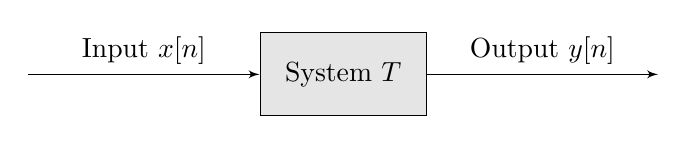
\begin{tikzpicture}[auto, node distance=4cm,>=latex']
      \node [input, name=input] {};
      \node [block, right of=input] (system) {System $T$};
      \node [output, right of=system] (output) {};

      \draw [draw,->] (input) -- node {Input $x[n]$} (system);
      \draw [->] (system) -- node {Output $y[n]$} (output);
    \end{tikzpicture}
  \end{center}
\item If input and output are not both CT or DT signals, it is a hybrid CT-DT system.
  \begin{center}
    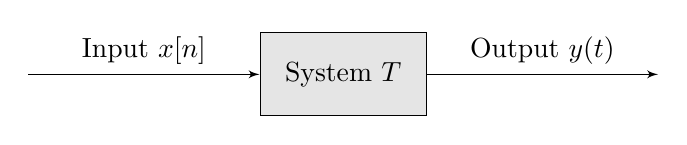
\begin{tikzpicture}[auto, node distance=4cm,>=latex']
      \node [input, name=input] {};
      \node [block, right of=input] (system) {System $T$};
      \node [output, right of=system] (output) {};

      \draw [draw,->] (input) -- node {Input $x[n]$} (system);
      \draw [->] (system) -- node {Output $y(t)$} (output);
    \end{tikzpicture}
  \end{center}
  \begin{center}
    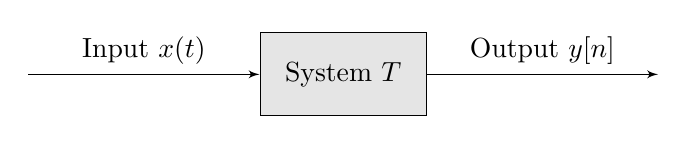
\begin{tikzpicture}[auto, node distance=4cm,>=latex']
      \node [input, name=input] {};
      \node [block, right of=input] (system) {System $T$};
      \node [output, right of=system] (output) {};

      \draw [draw,->] (input) -- node {Input $x(t)$} (system);
      \draw [->] (system) -- node {Output $y[n]$} (output);
    \end{tikzpicture}
  \end{center}
\end{itemize}

As a shorthand notation for the graphical description above we can use $x \mapsto y$. A system maps  a function $x$ to a function $y$:

\begin{itemize}
\item CT system
  \[
  x(t) \mapsto y(t)
  \]
  
\item DT system
  \[
  x[n] \mapsto y[n]
  \]
\item Hybrid CT-DT system
  \[
  x[n] \mapsto y(t)
  \]
  \begin{center}
    or
  \end{center}
  \[
  x(t) \mapsto y[n]
  \]
\end{itemize}

When a system has no input, the system is {\it autonomous}. An autonomous system just produces output: $\mapsto y$.

\begin{center}
  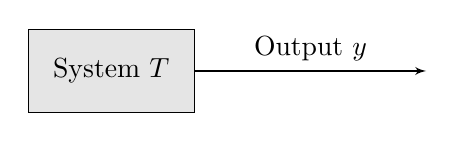
\begin{tikzpicture}[auto, node distance=4cm,>=latex']
    \node [input, name=input] {};
    \node [block, right of=input] (system) {System $T$};
    \node [output, right of=system] (output) {};

    \draw [->] (system) -- node {Output $y$} (output);
  \end{tikzpicture}
\end{center}

We can think of an autonomous system as a function generator, producing signals for use.

\section{CT system representations}

We can mathematically represent, or model, systems multiple ways.

\begin{itemize}
\item purely mathematically - in time domain we will use
  \begin{itemize}
  \item for CT systems: linear, constant coefficient differential equations. e.g.
    \[
    y^{\prime\prime} + ay^\prime + by = x
    \]
    
  \item for DT systems: linear, constant coefficient difference equation, e.g.
    \[
    y[n] = a y[n-1] + b y[n-2] + x[n]
    \]
  \end{itemize}
  or
  \begin{itemize}
  \item for CT systems: CT impulse response
  \item for DT systems: DT impulse response
  \end{itemize}
\item purely mathematically - in frequency domain we will use
  \begin{itemize}
  \item frequency response
  \item transfer function (complex frequency, covered in ECE 3704)
  \end{itemize}
\item graphically, using a mixture of math and block diagrams
\end{itemize}

Mathematical models:
\begin{itemize}
\item provide abstraction, removing (often) irrelevant detail.
\item can be more or less detailed, an {\it internal} v.s. {\it external} (block box) description
\item are not unique with respect to instantiation (implementation)
\item are limited to the regime they were designed for
\end{itemize}

\begin{example}[RC Circuit]
  Consider the RC circuit. It is a single input - single output system. We will be able to represent it mathematically or graphically and internally or externally.

  \begin{tabular}{ccc}
    & Graphical & Symbolic\\
    & & \\
    External &
    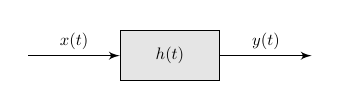
\begin{tikzpicture}[auto, node distance=3cm,>=latex',, scale=0.6, every node/.style={transform shape}]
      \node [input, name=input] {};
      \node [block, right of=input] (system) {$h(t)$};
      \node [output, right of=system] (output) {};

      \draw [draw,->] (input) -- node {$x(t)$} (system);
      \draw [->] (system) -- node {$y(t)$} (output);
    \end{tikzpicture}
    & $y(t) = h(t)*x(t)$\\
    Internal &
    \begin{circuitikz}[american voltages, scale=0.6, every node/.style={transform shape}]
      \draw
      (0,2) to[R, l=$R$] (3,2)
      (3,2) to[C, l=$C$] (3,0)
      (0,2) to[V, l_=$x(t)$] (0,0)
      (0,0) to[short] (3,0)
      (3,2) to[short, -o] (5,2)
      (3,0) to[short, -o] (5,0)
      (5,2) to[open, v=$y(t)$] (5,0);
    \end{circuitikz}

    & $y^\prime + \frac{1}{RC} y = \frac{1}{RC} x(t)$\\
  \end{tabular}
\end{example}

It does not matter what the underlying system implementation is. For example, consider a mechanical system, described by a second-order ODE:

\begin{center}
  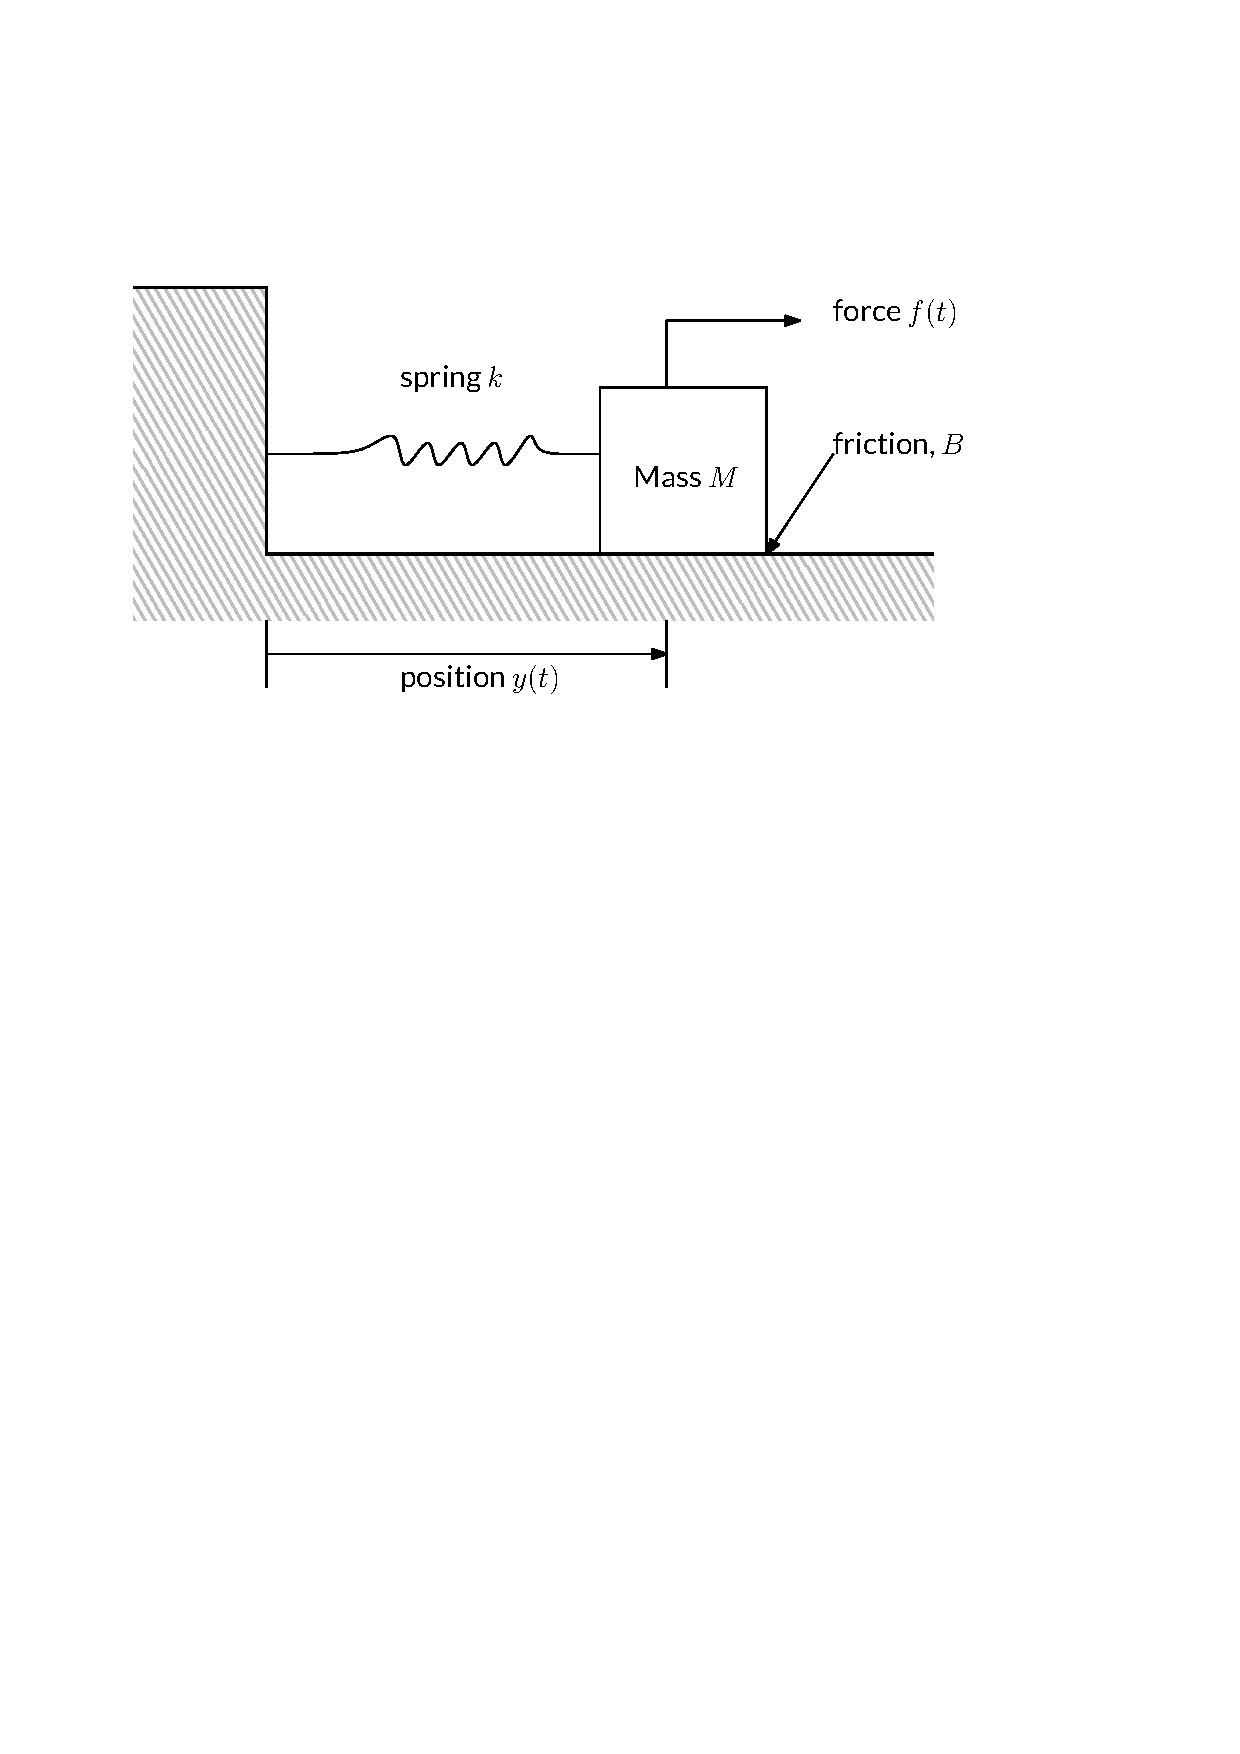
\includegraphics[scale=0.6]{graphics/mechanical_system.pdf}
\end{center}

\begin{tabular}{ll}
  $y$ = position & $M$ = mass\\
  $y^\prime$ = velocity & $K$ = spring constant\\
  $y^{\prime\prime}$ = acceleration & $B$ = coefficient of friction\\
\end{tabular}

\[
y^{\prime\prime} + \frac{B}{M} y^\prime + \frac{K}{M}y = \frac{1}{M}f(t)
\]

Compare this to the parallel RLC circuit, described by the second-order ODE:

\begin{center}
  \begin{circuitikz}[american voltages]
    \draw
    (0,0) to[american current source, l=$f(t)$] (0,2)
    (2,0) to[R, l=$R$] (2,2)
    (4,0) to[L, l=$L$] (4,2)
    (6,0) to[C, l=$C$] (6,2)
    (0,0) to[short, -o] (8,0)
    (0,2) to[short, -o] (8,2)
    (8,2) to[open, v=$y(t)$] (8,0);
  \end{circuitikz}
\end{center}

\begin{tabular}{ll}
  $y$ = voltage & $R$ = resistance\\
  $Cy^\prime$ = capacitor current & $L$ = inductance\\
  & $C$ = capacitance\\
\end{tabular}

\[
y^{\prime\prime} + \frac{1}{RC} y^\prime + \frac{1}{LC}y = \frac{1}{LC}f(t)
\]

Comparing these systems, if $R = \frac{1}{B}$, $L = \frac{1}{K}$, and $C = M$, they are mathematically identical.

\section{System properties and classification}

Choosing the right kind of system model is important. Here are some important properties that allow us to broadly classify systems.
\begin{itemize}
\item Memory
\item Invertability
\item Causality
\item Stability
\item Time-invariance
\item Linearity
\end{itemize}

Let's define each it turn.

\subsection{Memory}
The output of a system with memory depends on previous or future inputs and is said to be {\it dynamic}. Otherwise the system is memoryless or {\it instantaneous}, and the output $y(t)$ at time $t$ depends only on $x(t)$.
For example in CT:
\[
y(t) = 2x(t)
\]
is a memoryless system, while
\[
y(t) = \int\limits_{-\infty}^{t} x(\tau) \; dt
\]
has memory.

\subsection{Invertability}

A system is invertable if there exists a system that when placed in series with the original recovers the input.
\[
x(t) \mapsto{T} y(t) \mapsto{T^{-1}} x(t)
\]
where $T^{-1}$ is the inverse system of $T$. For example, consider a system
\[
x(t) \mapsto y(t) = \int\limits_{-\infty}^t x(\tau) \; d\tau
\]
and a system
\[
y(t) \mapsto z(t) = \frac{dy}{dt} 
\]
The combination in series $x(t) \mapsto y(t) \mapsto z(t) = x(t)$, i.e. the derivative undoes the integral.

\subsection{Causality}
A CT system is causal if the output at time $t$ depends on the input for time values at or before $t$:
\[
y(t) \;\text{depends on}\; x(\tau) \;\text{for} \; \tau \leq t
\]
All physical CT systems are causal, even if all continuous systems are not (e.g. continuous 2D images $f(u,v)$, have no "before" and "after").

For example, consider a CT system whose impulse response is $h(t) = e^{-t^2}$. This implies the system produces output \emph{before} (i.e. for $t < 0$) the impulse is applied at $t=0$, somehow anticipating the arrival of the impulse. Barring time-travel, this is physically impossible.

\subsection{Stability}

A CT system is (BIBO) stable if applying a bounded-input
\[
x(t) < \infty \; \forall \; t
\]
results in a bounded-output $x(t) \mapsto y(t)$ and 
\[
y(t) < \infty \; \forall \; t
\]
Note, bounded in practice is limited by the physical situation, e.g. positive and negative rails in a physical circuit.

For example, a CT system described by the LCCDE
\[
\frac{dy}{dt}(t) - 2y(t) = x(t)
\]
is unstable because the solution $y(t)$ will have one term of the form $Ce^{2t}$, for most non-zero inputs $x(t)$ or any non-zero initial condition, that grows unbounded as time increases.

\subsection{Time-invariance}
A CT system is time-invariant if, given
\[
x(t) \mapsto y(t)
\]
then a time-shift of the input leads to the same time-shift in the output
\[
x(t-\tau) \mapsto y(t-\tau)
\]

An important counterexample is a CT system described by a LCCDE, e.g.
\[
\frac{dy}{dt}(t) + y(t) = x(t)
\]
but non-zero auxillary conditions at some $t_0$, $y(t_0) = y_0 \neq 0$. Such systems will have a term in its solution that depends on $y_0$. However if I time shift the input, the term that depends on $y_0$ does not shift (since it is anchored to $t_0$) and the total output does not shift identically with the input. Thus the system cannot be time-invariant.

\subsection{Linearity}

A CT system is linear if the output due to a sum of scaled individual inputs is the same as the scaled sum of the individual outputs with respect to those inputs. In other words given
\[
x_1(t) \mapsto y_1(t) \;\text{and}\; x_2(t) \mapsto y_2(t)
\]
then
\[
a x_1(t) + b x_2(t) \mapsto a y_1(t) + b y_2(t)
\]
for constants $a$ and $b$.
Note this property extends to sums of arbitrary signals, e.g. if
\[
x_i(t) \mapsto y_i(t) \; \forall\; i \in [1 \cdots N]
\]
then given $N$ constants $a_i$, if the system is linear
\[
\sum\limits_{i = 1}^N a_i x_i(t) \mapsto \sum\limits_{i = 1}^N a_i y_i(t) 
\]
This is a very important property, called {\it superposition}, and it simplifies the analysis of systems greatly.

Similar to time-invariance an important non-linear system is that is described by a LCCDE with non-zero auxillary conditions at some $t_0$, $y(t_0) = y_0$. Again such systems will have a term in it's solution that depends on $y_0$. Given two inputs, each individual response will have that term in it, so thier sum has double that term. However the response due to the sum of the inputs would again only have one and the sum of the responses would not be the same as the response of the sum. Such a system cannot be linear.

\section{Stable LTI Systems}

The remainder of this course is about stable, linear, time-invariant (LTI) systems. As we have seen in CT such systems can be described by a LCCDE with zero auxillary (initial) conditions (the system is \emph{at rest}). 

We have seen previously how to find the impulse response, $h(t)$, of such systems. We now note some relationships between the impulse response and the system properties described above.

\begin{itemize}
\item If a system is memoryless then $h(t) = C \delta(t)$ for some constant $C$.
\item If a system is causal then  $h(t) = 0$ for $t < 0$.
\item If a system is BIBO stable then
  \[
  \int\limits_{-\infty}^{\infty} |h(t)| \; dt < \infty
  \]
\end{itemize}


\newpage
\chapter{Linear time invariant DT systems}

\section{DT system representations}

We can mathematically represent, or model, DT systems multiple ways.

\begin{itemize}
\item purely mathematically - in time domain we will use

  \begin{itemize}
  \item linear, constant coefficient difference equations, e.g.
    \[
    y[n] = a y[n-1] + b y[n-2] + x[n]
    \]
  \item DT impulse response $h[n]$
  \end{itemize}
\item purely mathematically - in frequency domain we will use
  \begin{itemize}
  \item frequency response
  \item transfer function (complex frequency, covered in ECE 3704)
  \end{itemize}
\item graphically, using a mixture of math and block diagrams
\end{itemize}

\section{System properties and classification}

Choosing the right kind of system model is important. Here are some important properties that allow us to broadly classify systems.
\begin{itemize}
\item Memory
\item Invertability
\item Causality
\item Stability
\item Time-invariance
\item Linearity
\end{itemize}

Let's define each it turn.

\subsection{Memory}
The output of a DT system with memory depends on previous or future inputs and is said to be {\it dynamic}. Otherwise the system is memoryless or {\it instantaneous}, and the output $y[n]$ at index $n$ depends only on $x[n]$.
For example:
\[
y[n] = 2x[n]
\]
is a memoryless system, while
\[
y[n+1] + y[n] = x[n]
\]
has memory. To  see this, write the difference equation in recursive form
\[
y[n] = -y[n-1] + x[n-1]
\]
and we see explicitly the current output $y[n]$ depends on past values of output and input.

\subsection{Invertability}

A system is invertible if there exists a system that when placed in series with the original recovers the input.
\[
x[n] \mapsto{T} y[n] \mapsto{T^{-1}} x[n]
\]
where $T^{-1}$ is the inverse system of $T$. For example, consider a system
\[
x[n] \mapsto y[n] = \sum\limits_{m=-\infty}^{n} x[m]
\]
and a system
\[
y[n] \mapsto z[n] = y[n] - y[n-1]
\]
The combination in series $x[n] \mapsto y[n] \mapsto z[n] = x[n]$, since
\[
z[n] = y[n] - y[n-1] = \sum\limits_{m=-\infty}^{n} x[m] - \sum\limits_{m=-\infty}^{n-1} x[m] = x[n]
\]
i.e. the difference undoes the accumulation.

\subsection{Causality}
A DT system is causal if the output at index $n$ depends on the input for index values at or before $n$:
\[
y[n] \;\text{depends on}\; x[m] \;\text{for} \; m \leq n
\]
While all physical CT systems are causal, practical DT systems may not be since we can used memory to "shift time". For CT systems we cannot store the infinite number of values between two time points $t_1$ and $t_2$, but we can store the $n_2-n_1$ values of a DT system between between two indices $n_1$ and $n_2$ (assuming infinite precision).

\begin{example}
Consider a DT system whose difference equation is
\[
y[n] = -x[n-1] + 2x[n] - x[n+1]
\]
We see the current output $y[n]$ depends on a "future" value of the input $x[n+1]$. Thus the system \textbf{is not} causal. In practice we can shift the difference equation to
\[
y[n-1] = -x[n-2] + 2x[n-1] - x[n]
\]
and then delay the output by one sample to get $y[n]$.
\end{example}

\begin{example}
Consider a DT system whose difference equation is
\[
y[n] = -y[n-1] + 2x[n]
\]
We see the current output $y[n]$ depends on a "past" value of the output $y[n-1]$ and the current input $x[n]$. Thus the system \textbf{is} causal. In practice we can immediately compute $y[n]$ with no delay. 
\end{example}

\subsection{Stability}

A DT system is (BIBO) stable if applying a bounded-input
\[
x[n] < \infty \; \forall \; n
\]
results in a bounded-output $x[n] \mapsto y[n]$ and 
\[
y[n] < \infty \; \forall \; n
\]
Note, bounded in practice is limited by the physical situation, e.g. the number of bits used to store values.

For example, a DT system described by the LCCDE
\[
y[n+1] - 2 y[n] = x[n+1]
\]
is unstable because the solution $y[n]$ will have one term of the form $\left( 2\right)^n$, for most non-zero inputs $x[n]$ or any non-zero initial condition, that grows unbounded as $n$ increases.

\subsection{Time-invariance}
A DT system is time(index)-invariant if, given
\[
x[n] \mapsto y[n]
\]
then an index-shift of the input leads to the same index-shift in the output
\[
x[n-m] \mapsto y[n-m]
\]

An important example is a DT system described by a LCCDE, e.g.
\[
y[n+1] - \frac{1}{2} y[n] = x[n+1]
\]
or in recursive form
\[
y[n] = \frac{1}{2} y[n-1] + x[n]
\]

If we index shift the input $x[n - m]$ we replace $n$ by $n-m$ and the difference equation becomes
\[
y[n-m+1] - \frac{1}{2} y[n-m] = x[n-m+1]
\]
which has the same solution shifted by $m$
\[
y[n-m] = \frac{1}{2} y[n-m -1] + x[n-m]
\]

If a coefficient depends on $n$ however, e.g
\[
y[n+1] - \frac{n}{2} y[n] = x[n+1]
\]
so that it is no longer LCC then the solution depends on $m$ and the system is no longer time-invariant.

\subsection{Linearity}

A DT system is linear if the output due to a sum of scaled individual inputs is the same as the scaled sum of the individual outputs with respect to those inputs. In other words given
\[
x_1[n] \mapsto y_1[n] \;\text{and}\; x_2[n] \mapsto y_2[n]
\]
then
\[
a x_1[n] + b x_2[n] \mapsto a y_1[n] + b y_2[n]
\]
for constants $a$ and $b$.
Note this property extends to sums of arbitrary signals, e.g. if
\[
x_i[n] \mapsto y_i[n] \; \forall\; i \in [1 \cdots N]
\]
then given $N$ constants $a_i$, if the system is linear
\[
\sum\limits_{i = 1}^N a_i x_i[n] \mapsto \sum\limits_{i = 1}^N a_i y_i[n] 
\]
This is a very important property, called {\it superposition}, and it simplifies the analysis of systems greatly.

An important non-linear system is that is described by a LCCDE with non-zero auxiliary conditions at some $n_0$, $y[n_0] = y_0$. As in CT, such systems will have a term in it's solution that depends on $y_0$. Given two inputs, each individual response will have that term in it, so their sum has double that term. However the response due to the sum of the inputs would again only have one and the sum of the responses would not be the same as the response of the sum. Such a system cannot be linear. Thus the system must be "at rest" before applying the input in order to be a linear system.

\section{Stable LTI Systems}

The remainder of this course is about stable, linear, time-invariant (LTI) systems. As we have seen in DT such systems can be described by a LCCDE with zero auxiliary (initial) conditions (the system is \emph{at rest}). 

We have seen previously how to find the impulse response, $h[n]$, of such systems. We now note some relationships between the impulse response and the system properties described above.

\begin{itemize}
\item If a system is memoryless then $h[n] = C \delta[n]$ for some constant $C$.
\item If a system is causal then  $h[n] = 0$ for $n < 0$.
\item If a system is BIBO stable then
  \[
  \sum\limits_{-\infty}^{\infty} |h[n]| < \infty
  \]
\end{itemize}


\newpage
\section{CT Convolution}

\subsection{Review CT LTI systems and superposition property}

Recall the superposition property of LTI systems. If a CT system is LTI then the superposition property holds. Given a system where
\[   
x_i(t) \mapsto y_i(t) \; \forall\; i
\]
then
\[
\sum\limits_{i} a_i x_i(t) \mapsto \sum\limits_{i} a_i y_i(t) 
\]

Superposition enables a powerful problem reduction strategy. The overall idea for is that if:

\begin{itemize}
\item we can write an aribtrary signal as a sum of simple signals, and 
\item we can determine the response to the simple signals, then
\item we can easily express the output due to the input using superposition
\end{itemize}

This will be a recurring pattern in this course. In this lecture, the simple signals are weighted, time shifts of one signal, the delta function, $\delta(t)$.

\subsection{Convolution Integral}

To derive this we start with the sifting property of the CT impulse function (from lecture 2)
\[
\int\limits_{a}^{b} x(t)\delta(t-t_0) \; dt = x(t_0)
\]
for any $a < t_0 < b$. A slight change of variables ($t_0 \rightarrow \tau$) and limits ($a \rightarrow -\infty$ and $b \rightarrow \infty$) gives:
\[
x(t) = \int\limits_{-\infty}^{\infty} x(\tau)\delta(t-\tau) \; d\tau
\]
showing that we can write any CT signal as an infinite sum (integral) of weighted and time-shifted impluse functions.

Let $h(t)$ be the CT {\it impulse response}, the output due to the input $\delta(t)$, i.e. $\delta(t) \mapsto h(t)$. Then if the system is time-invariant: $\delta(t-\tau) \mapsto h(t-\tau)$ and by superposition if the input is writen as
\[
x(t) = \int\limits_{-\infty}^{\infty} x(\tau)\delta(t-\tau) \; d\tau
\]
then the output is given by
\[
  y(t) = \int\limits_{-\infty}^{\infty} x(\tau)h(t-\tau) \; d\tau = x(t) * h(t)
\]
This is called the \emph{convolution integral}.

It is worth pausing here to see the signifigance. For a LTI CT system, if I know it's impulse response $h(t)$, I can find the response due to \textbf{any} input using convolution. For this reason the impulse response is another way to represent an LTI system.

\subsection{Graphical View of the Convolution Integral.}

Lets break the convolution expression down into pieces. In it's general form the convolution of two signals $x_1(t)$ and $x_2(t)$ is
\[
x_1(t) * x_2(t) = \int\limits_{-\infty}^{\infty} x_1(\tau)x_2(t-\tau) \; d\tau
\]

Suppose $x_1(t)$ and $x_2(t)$ are signals that look like
\begin{center}
  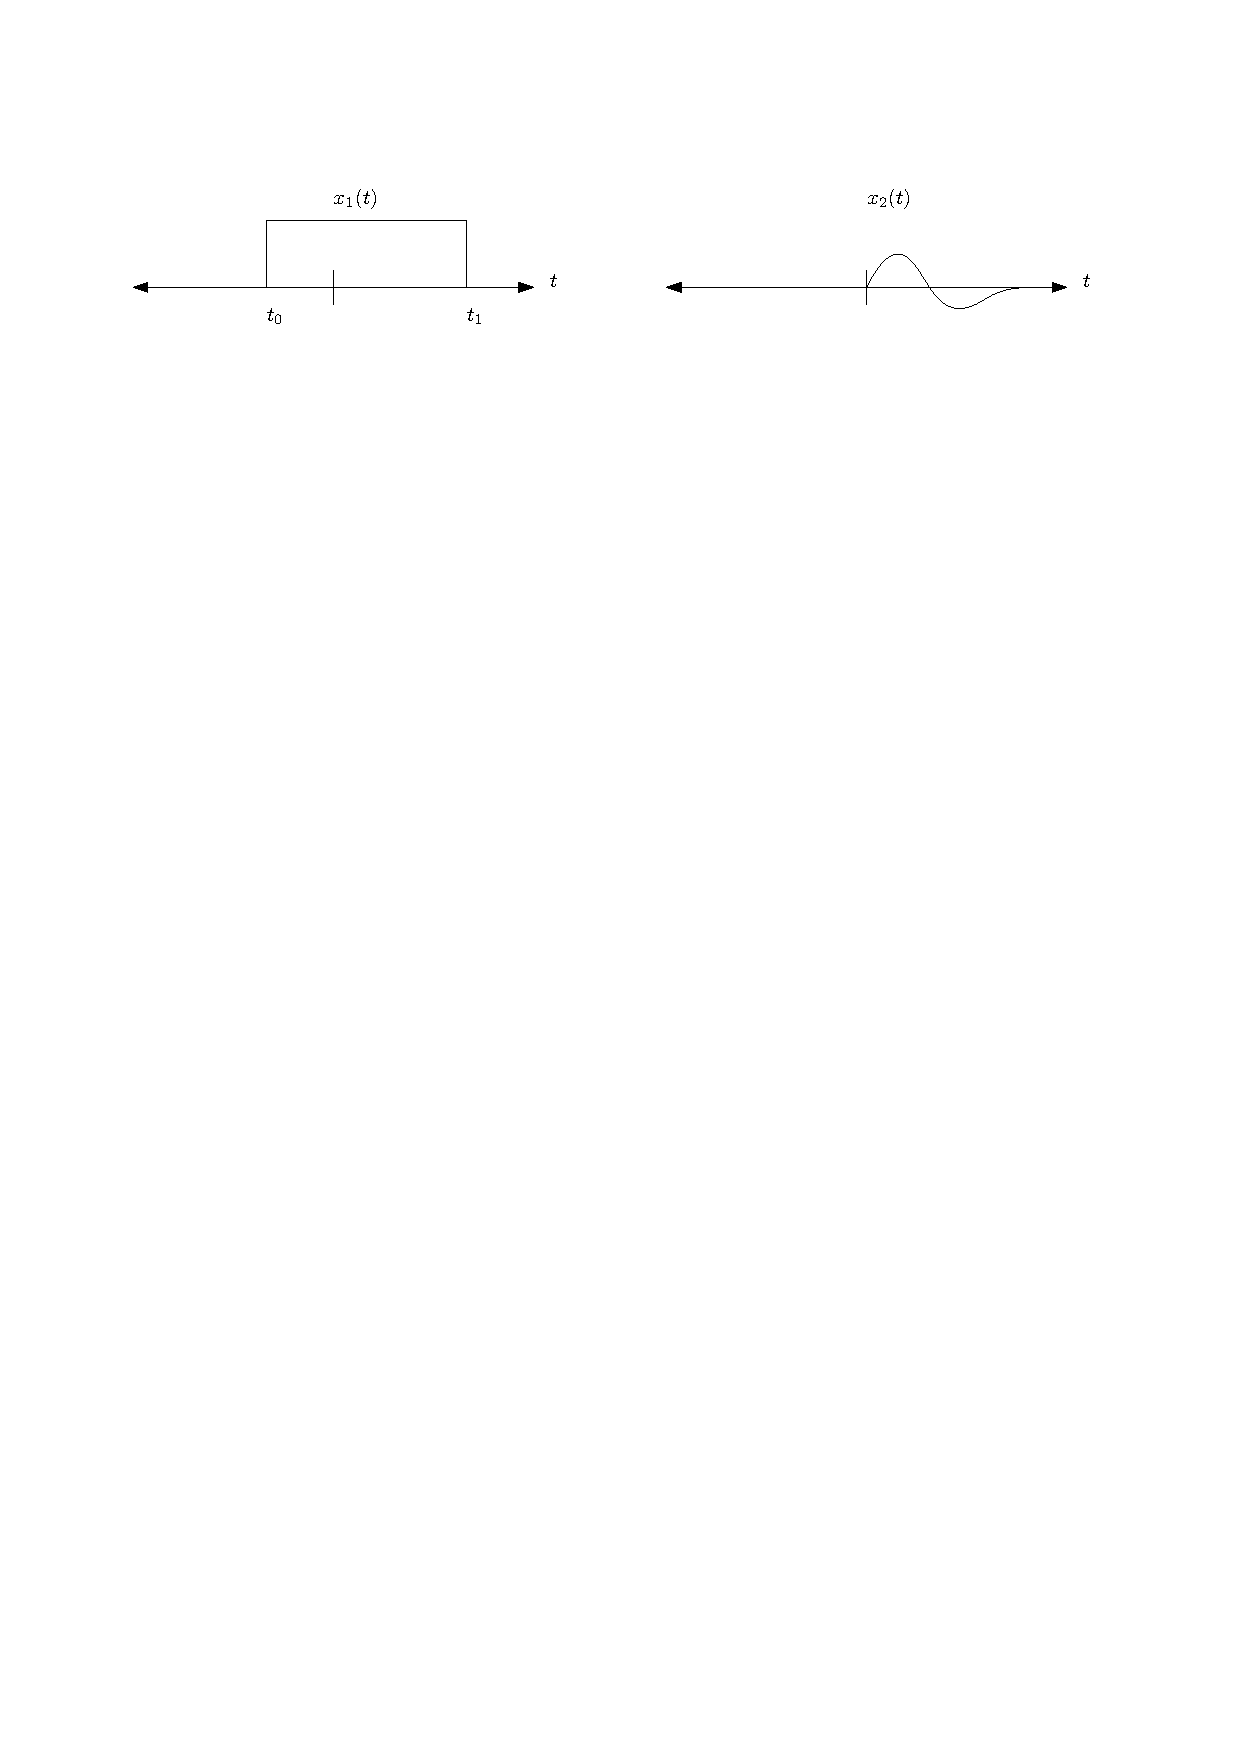
\includegraphics[scale=1]{graphics/convolution-explain1.pdf}
\end{center}

Then $x_1(\tau)$ and $x_2(-\tau)$ look like
\begin{center}
  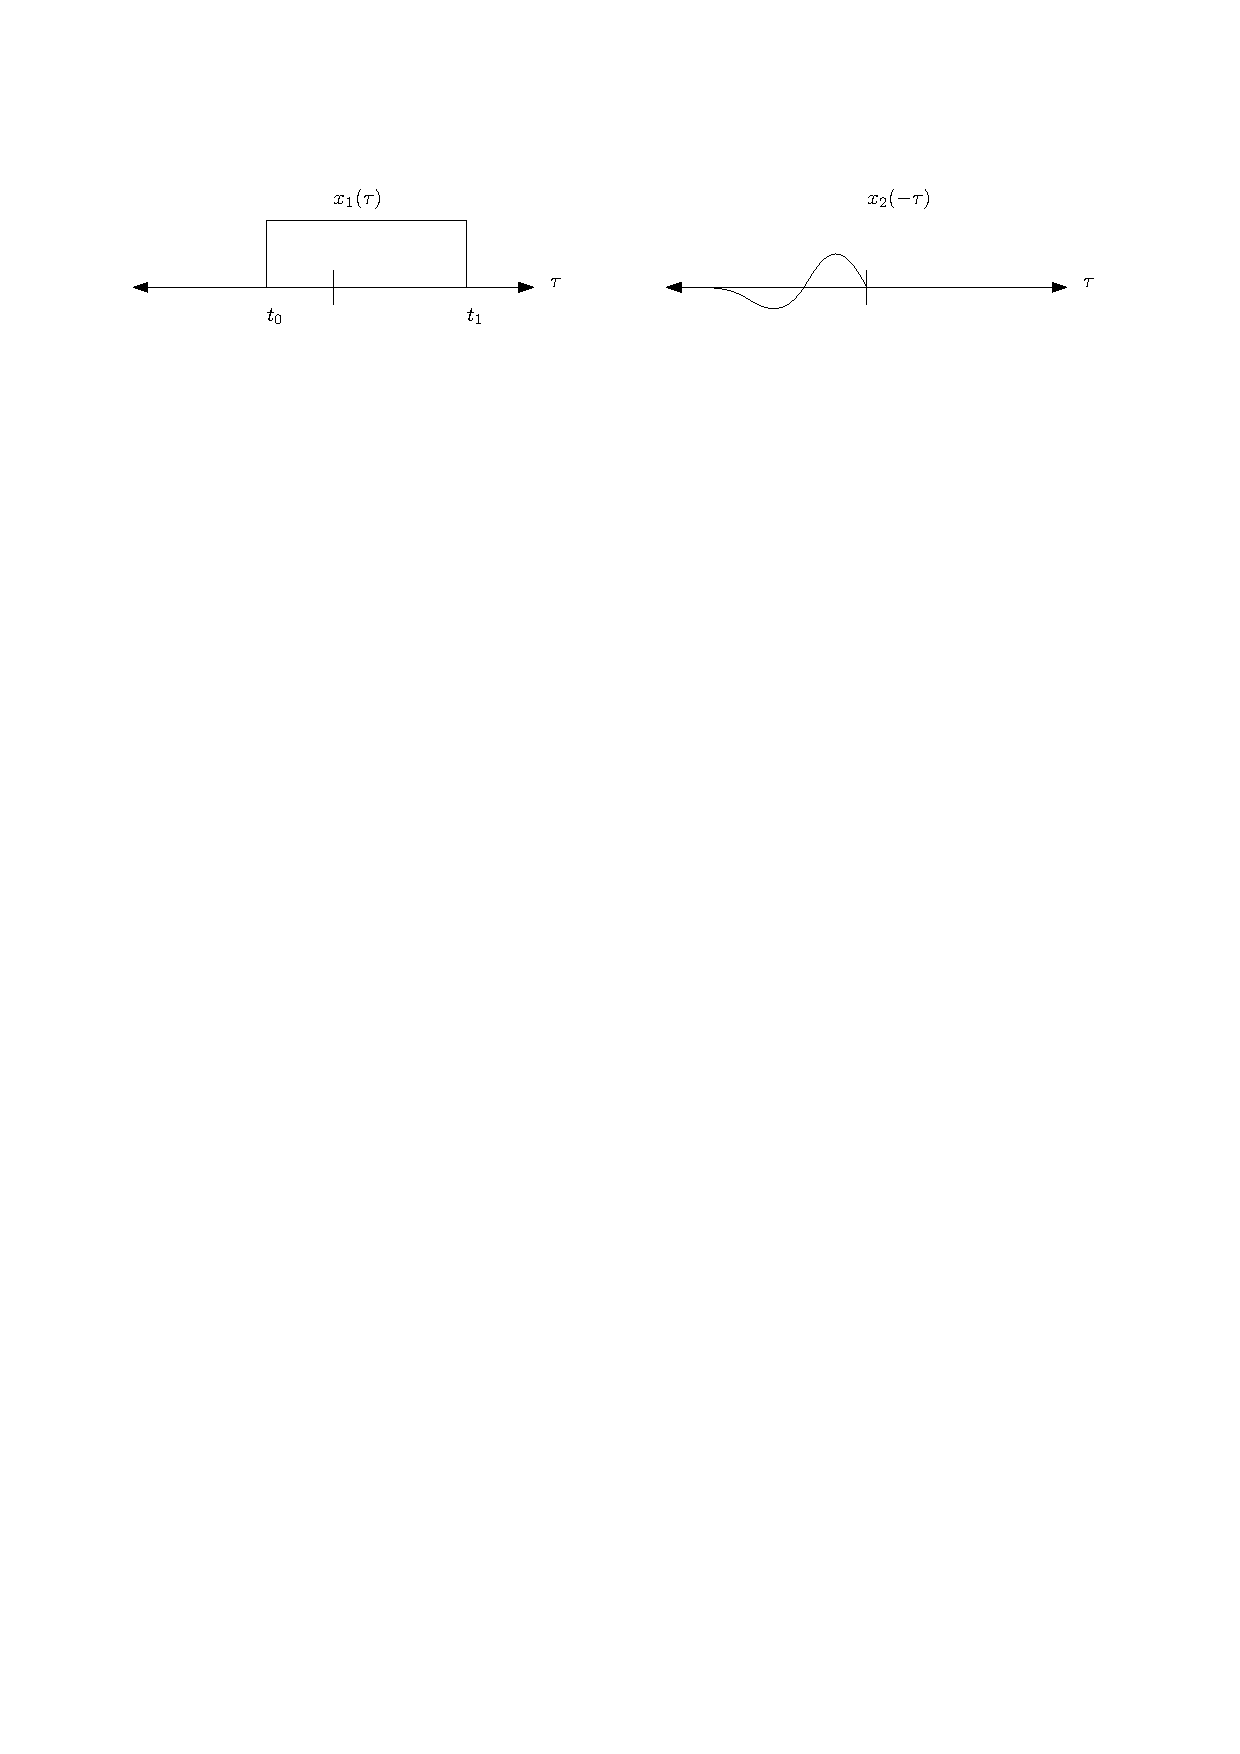
\includegraphics[scale=1]{graphics/convolution-explain2.pdf}
\end{center}
The signal $x_2(t-\tau)$ is $x_2(-\tau)$ shifted by $t$ (since $x_2(-\tau+t)= x_2(t-\tau)$) and then looks like
\begin{center}
  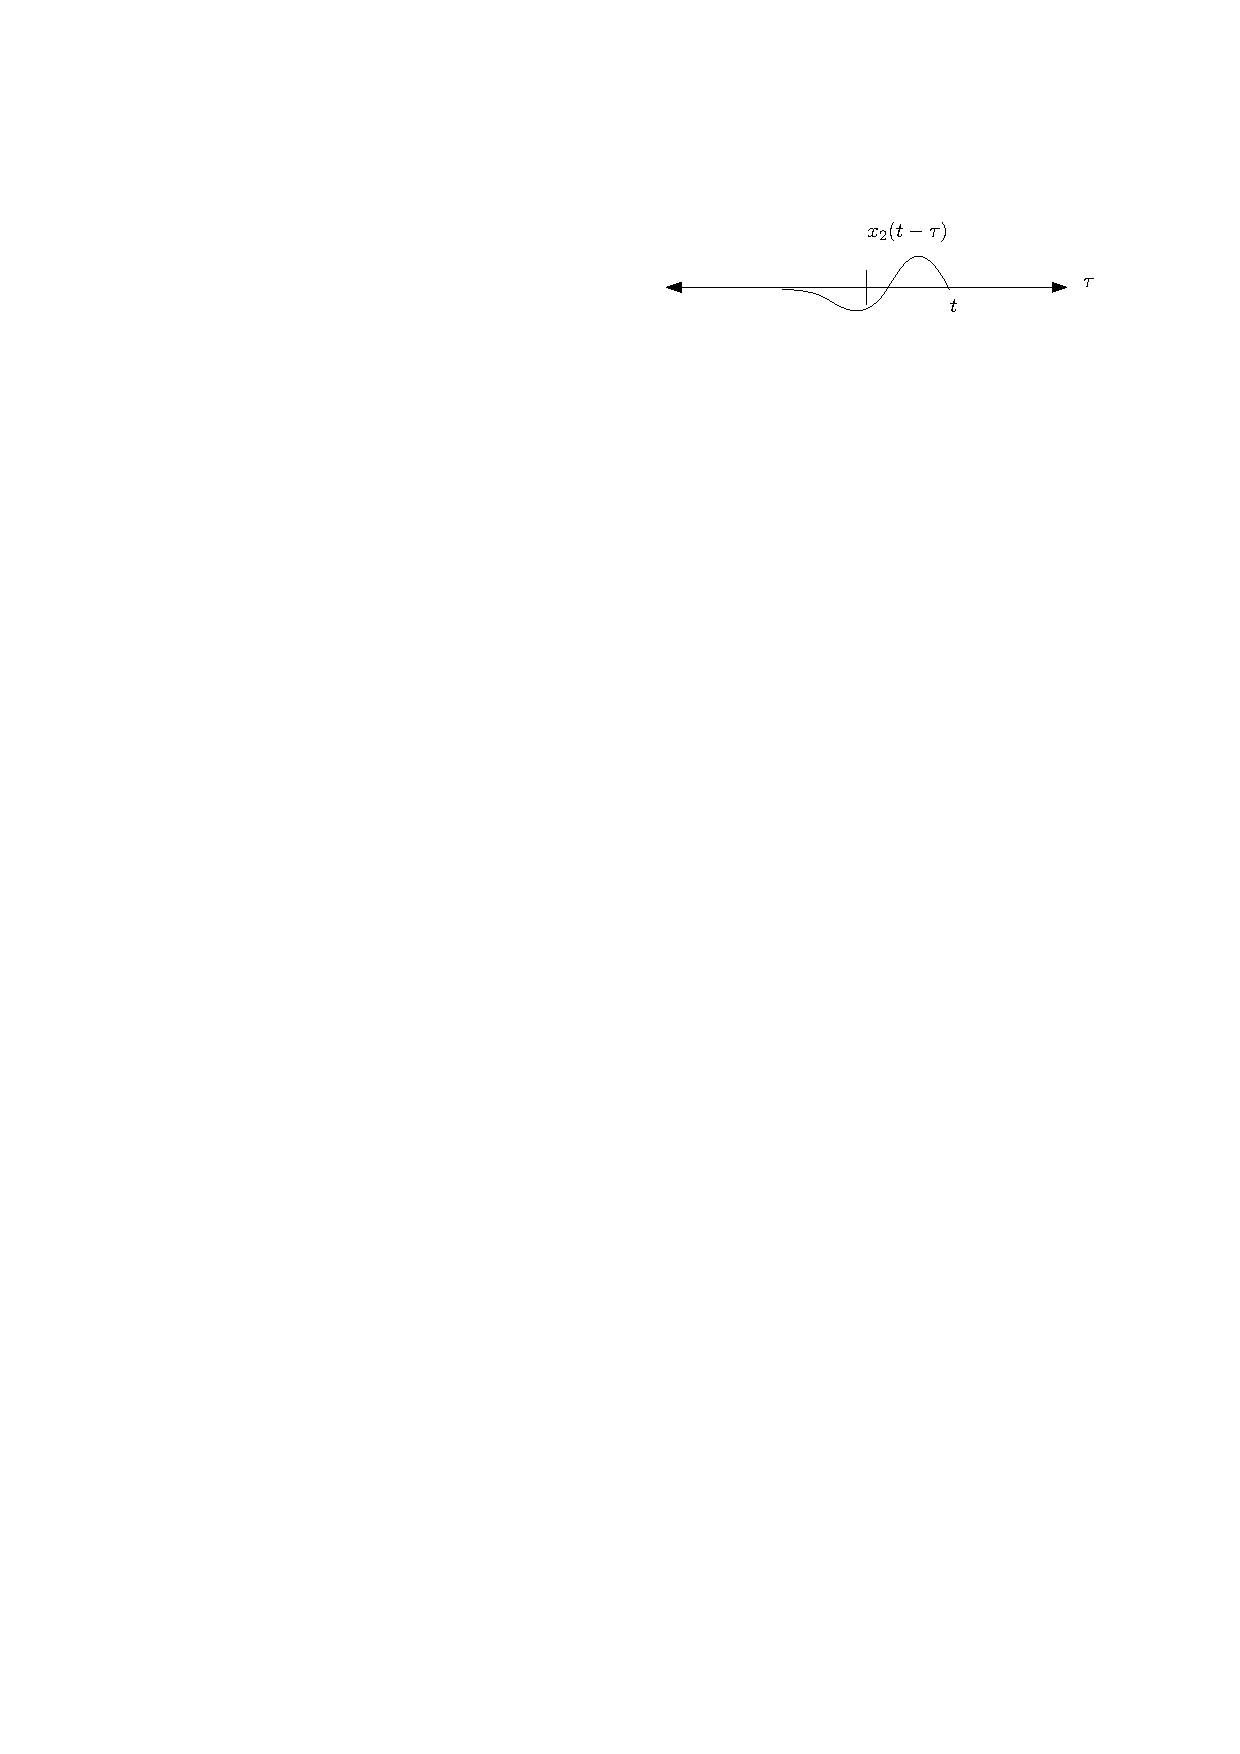
\includegraphics[scale=1]{graphics/convolution-explain3.pdf}
\end{center}
Then the integrand of convolution is the product $x_1(\tau)x_2(t-\tau)$ whose plot depends of the value of $t$. Some examples, where the individual signals are dashed and their product is in bold:
\begin{center}
  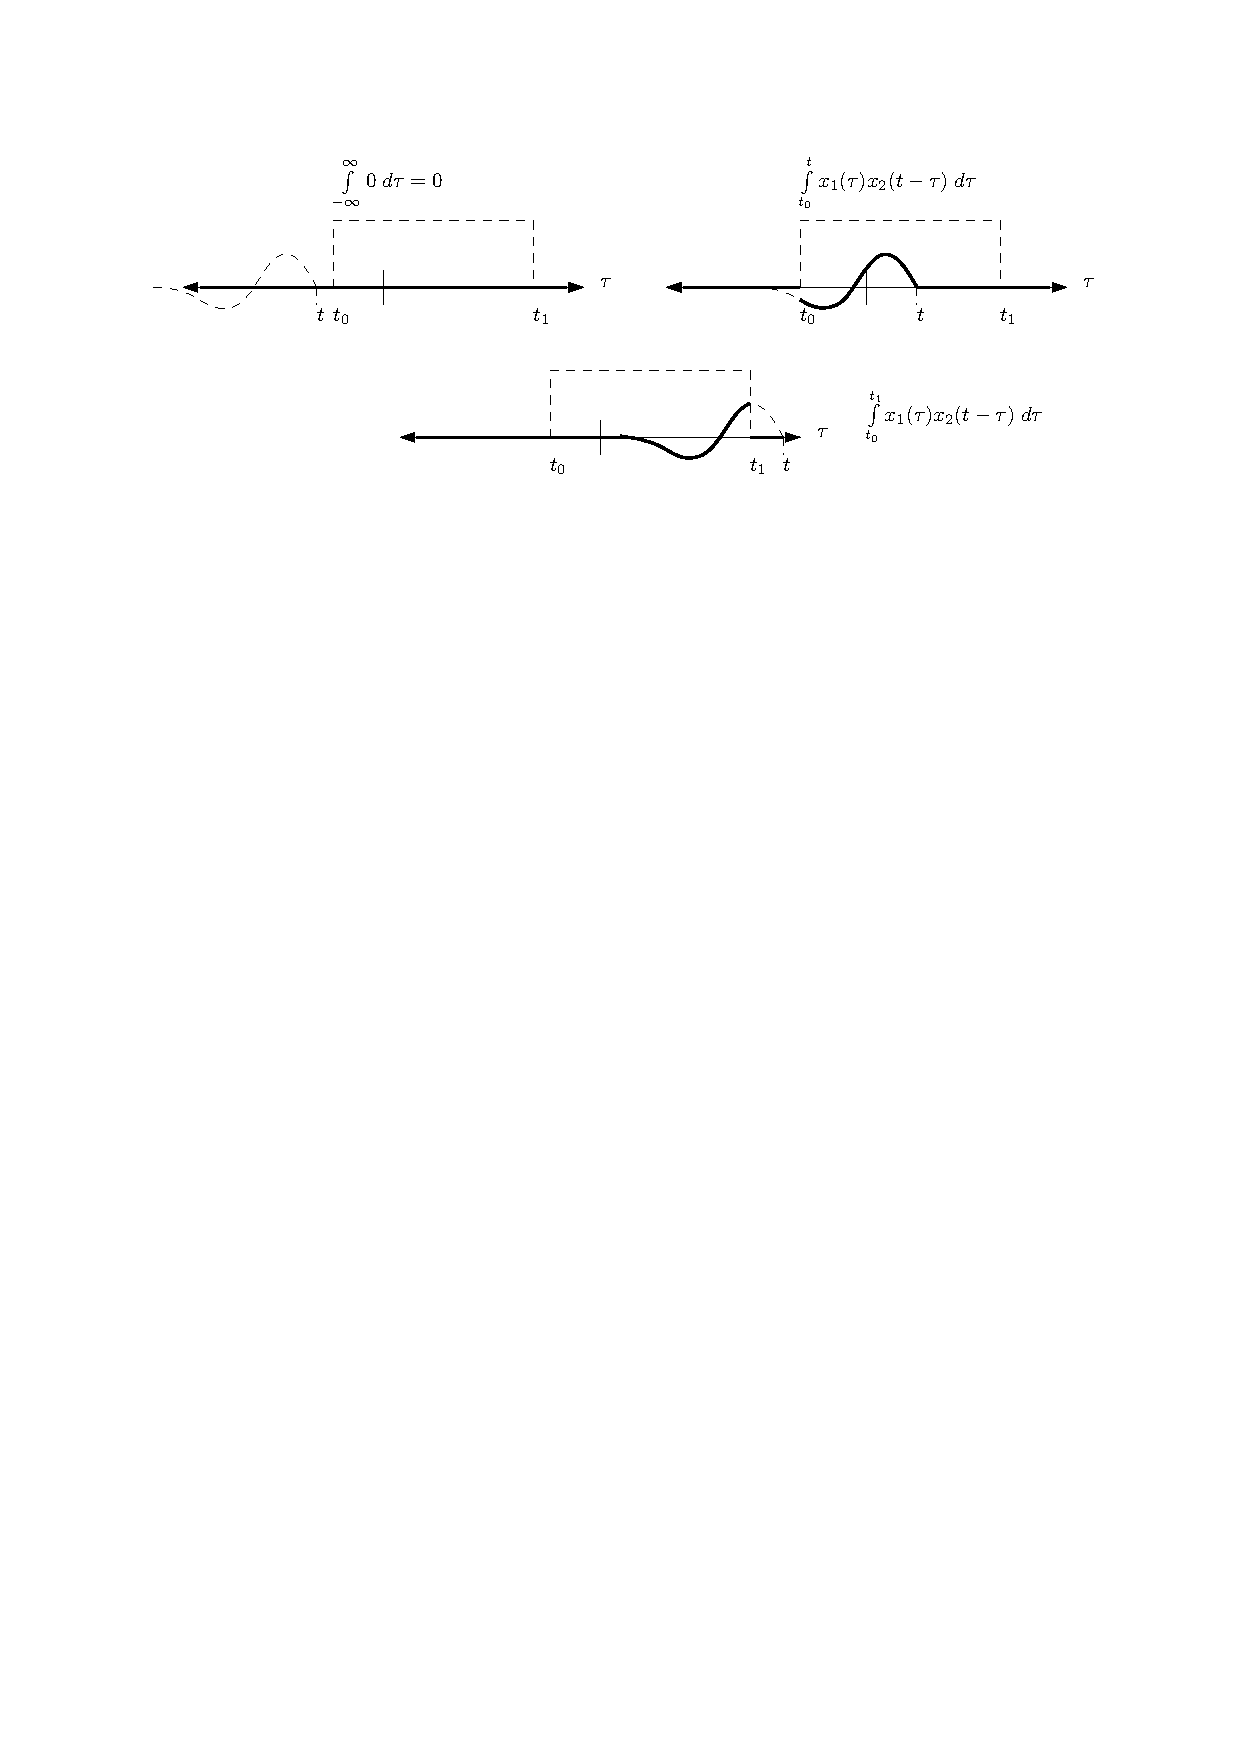
\includegraphics[scale=1]{graphics/convolution-explain4.pdf}
\end{center}
Then convolution is the total integral of the product (bold curves above) for that value of $t$. For the example above we see the integral will be zero for $t$ less than $t_0$ since the two signals do not overlap and their product is zero. For $t_0 < t < t_1$ the signals overap and the product is non-zero, and the effective bounds of integration are $[t_0,t]$. For $t > t_1$ the signals again overap and the product is non-zero, but the effective bounds of integration are $[t_0,t_1]$. 

\subsection{Examples of CT Convolution}

\begin{example}[$u(t) * u(t)$] Consider the convolution of two unit step functions.
  \[
  u(t) * u(t) = \int\limits_{-\infty}^{\infty} u(\tau)u(t-\tau) \; d\tau
  \]
  The product $u(\tau) u(t-\tau)$ is non-zero only when $t\geq 0$ as illustrated here
  \begin{center}
  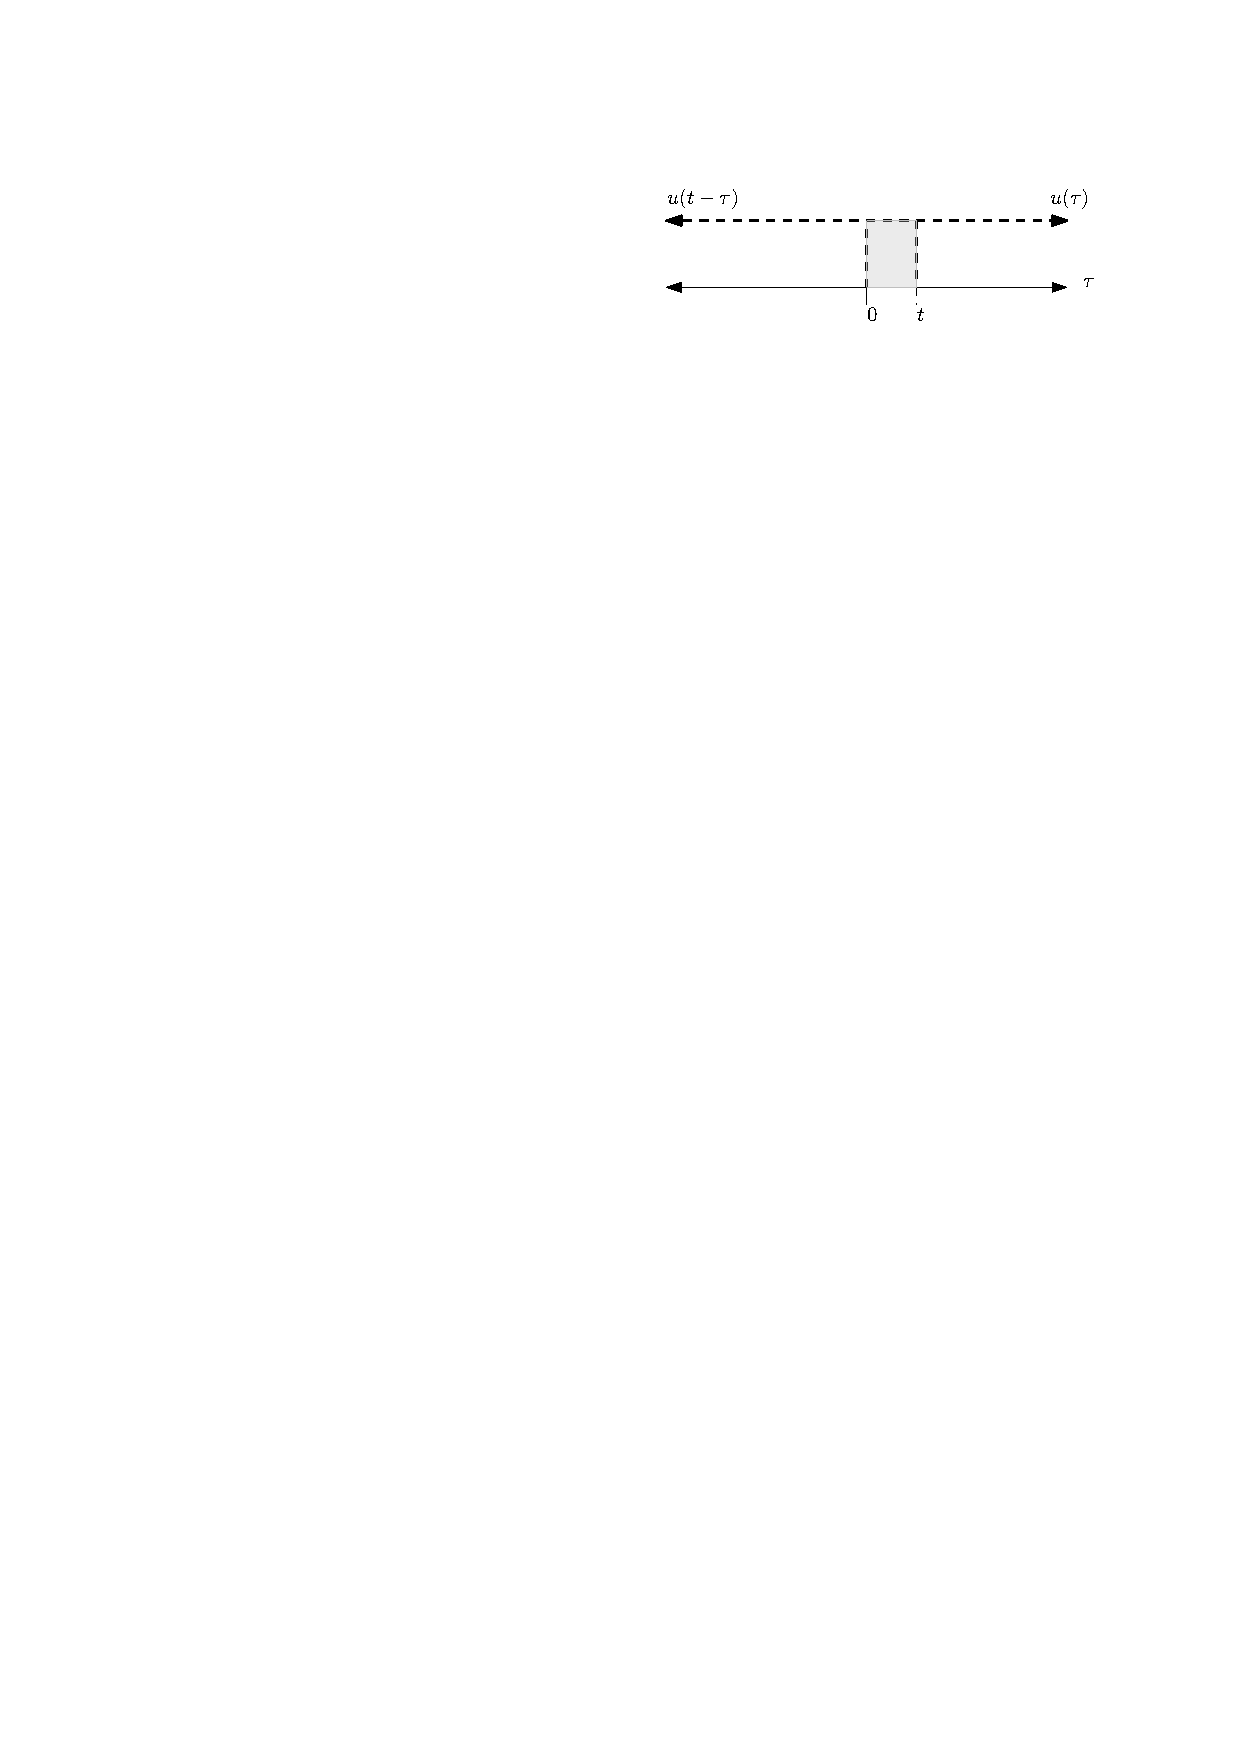
\includegraphics[scale=1]{graphics/convolution-step.pdf}
\end{center}
  The convolution integral is then the shaded area
  \[
u(t) * u(t) = \left\{ \begin{array}{lc}
  0 & t< 0\\
  \int\limits_{0}^{t} d\tau = t  & t \geq 0\\
\end{array}\right.
\]
Combining this back into a single expression gives:
\[
u(t) * u(t) = tu(t)
\]
Thus the convolution of two step signals is a ramp signal.\\$\blacksquare$
\end{example}

\begin{example}[$u(t) * e^{-at}u(t)$] Let $x_1(t) = u(t)$ and $x_2(t) = e^{-at}u(t)$ for constant $a\in\mathbb{C}$, then
  \[
u(t) * e^{-at}u(t) = \int\limits_{-\infty}^{\infty} u(\tau)e^{-a(t-\tau)}u(t-\tau) \; d\tau
\]
Similar to the previous example, the product $u(\tau) e^{-a(t-\tau)} u(t-\tau)$ is non-zero only when $t\geq 0$
  \begin{center}
  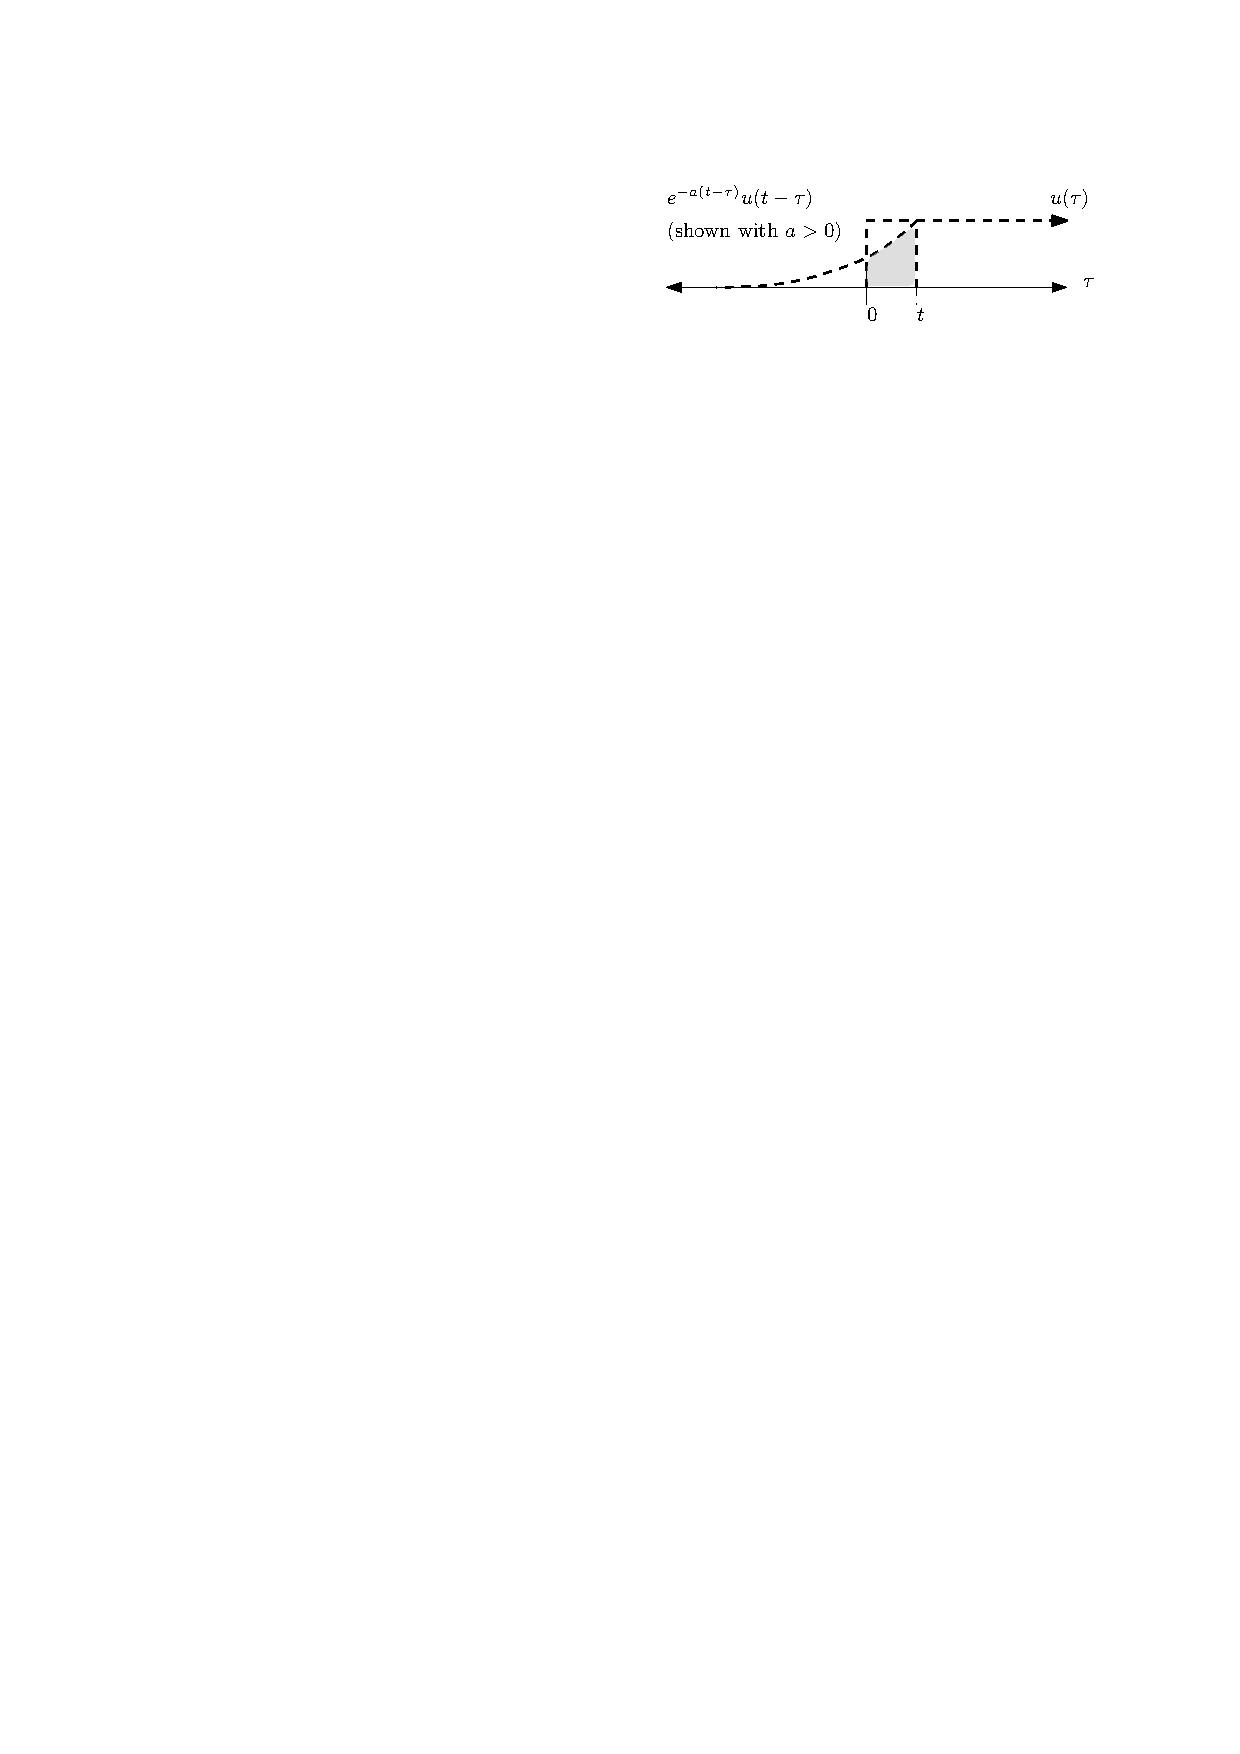
\includegraphics[scale=1]{graphics/convolution-expstep.pdf}
  \end{center}
  The convolution integral is then the shaded area
  \[
u(t) * e^{-at}u(t) = \left\{ \begin{array}{lc}
  0 & t< 0\\
  \int\limits_{0}^{t} e^{-a(t-\tau)} d\tau = \frac{1-e^{-at}}{a}  & t \geq 0\\
\end{array}\right.
\]
Combining this back into a single expression gives:
\[
u(t) * e^{-at}u(t) = \frac{1-e^{-at}}{a}u(t)
\]
$\blacksquare$
\end{example}

\begin{example}[Convolution with a delta function] Let $x_1(t) = \delta(t)$ and $x_2(t)$ be an arbitrary signal. Then
  \[
  \delta(t) * x_2(t) = \int\limits_{-\infty}^{\infty} \delta(\tau)x_2(t-\tau) \; d\tau
  \]
  By the sifting property of the delta function this evaluates to
  \[
  \delta(t) * x_2(t) = x_2(t)
  \]
  or in other words convolution with a delta function just results in the signal it was convolved with. That is it acts like the identity function, with respect to convolution.\\
  $\blacksquare$
\end{example}

The following table lists several convolution results.

\begin{center}
  Short Table of Representative Convolution Integrals
  \vspace{1em}
  
\bgroup
\def\arraystretch{2}
\setlength\tabcolsep{2em}
\begin{tabular}{|c|c|c|}
  \hline
  $x_1(t)$ & $x_2(t)$ & $x_1(t) * x_2(t)$\\
  \hline
  \hline
  $e^{a t}u(t)$ & $u(t)$ & $\frac{1-e^{a t}}{-a}u(t)$\\
  $u(t)$ & $u(t)$ & $tu(t)$\\
  $e^{a_1 t}u(t)$ & $e^{a_2 t}u(t)$ & $\frac{e^{a_1 t}-e^{a_2 t}}{a_1 - a_2}u(t)$ for $a_1 \neq a_2$\\
  $e^{a t}u(t)$ & $e^{a t}u(t)$ & $te^{a t}u(t)$\\
  $te^{a_1 t}u(t)$ & $e^{a_2 t}u(t)$ & $\frac{e^{a_2 t}-e^{a_1 t} + (a_1-a_2)te^{a_1 t}}{(a_1 - a_2)^2}u(t)$ for $a_1 \neq a_2$\\
  $e^{a_1 t}\cos(\beta t + \theta)u(t)$ & $e^{a_2 t}u(t)$ & $\frac{\cos(\theta - \phi)e^{a_2 t} - e^{a_1 t}\cos(\beta t + \theta - \phi)}{\sqrt{(a_1 + a_2)^2 + \beta^2}}u(t)$\\
  & & $\phi = \arctan\left( \frac{-\beta}{a_1 + a_2}\right)$\\
\hline                       
\end{tabular}
\egroup

\end{center}

\subsection{Properties of CT Convolution}
There are several useful properties of convolution. We do not prove these here, but it is not terribly difficult to do so. Given signals $x_1(t)$, $x_2(t)$, and $x_3(t)$:

\begin{description}
\item [Communative Property] The ordering of the signals does not matter.
  \[
x_1(t) * x_2(t) = x_2(t) * x_1(t)
  \]
\item [Distributive Propery] Convolution is distributed over addition.
  \[
  x_1(t) * \left[x_2(t) + x_3(t)\right] = \left[x_1(t) * x_2(t) \right] + \left[x_1(t) * x_3(t) \right] 
  \]
\item [Associative Property] The order of convolution does not matter.
    \[
  x_1(t) * \left[x_2(t) * x_3(t)\right] = \left[x_1(t) * x_2(t) \right] * x_3(t) 
  \]
\item [Time Shift] Given $x_3(t) = x_1(t) * x_2(t)$ then for time shifts $\tau_1, \tau_2 \in \mathbb{R}$
  \[
  x_1(t-\tau_1) * x_2(t-\tau_2) = x_3(t-\tau_1 - \tau_2)
  \]
\item [Multiplicative Scaling] Given $x_3(t) = x_1(t) * x_2(t)$ then for constants $a,b \in \mathbb{C}$
  \[
  \left[a\, x_1(t)\right] * \left[b\, x_2(t)\right] = a\, b\, x_3(t)
  \]
\end{description}

These properties can be used in combination with a table like that above to compute the convolution of a wide variety of signals without evaluating the integrals.

\begin{example} Here is a simple example. Let $x_1(t) = e^tu(t)$ and $x_2(t) = 2\delta(t) + 5e^{-3t}u(t)$.
  \[
  x_1(t) * x_2(t) =  e^tu(t) * \left[2\delta(t) + 5e^{-3t}u(t)\right] 
  \]
  Using the distributive property
  \[
  x_1(t) * x_2(t) =  2\left[\delta(t) * e^tu(t)\right]  + 5\left[e^tu(t) * e^{-3t}u(t)\right]
  \]
  Using previously derived results involving the delta function and the table row 3
  \[
  x_1(t) * x_2(t) = 2 e^t\, u(t) + 5\left[ \frac{e^t-e^{-3t}}{4}\right]u(t)
  \]
  Doing some simplification gives the result
  \[
  x_1(t) * x_2(t) = \left[ \frac{13}{4}e^t-\frac{5}{4}e^{-3t}\right]u(t)
  \]
  
$\blacksquare$
\end{example}

\begin{example} Here is a more complicated example. Let $x_1(t) = 2e^{-5t}u(t-1)$ and $x_2(t) = \left(1-e^{-t}\right)u(t)$.
  \[
  x_1(t) * x_2(t) = \left[2e^{-5t}u(t-1)\right] * \left[\left(1-e^{-t}\right)u(t)\right]
  \]
  We first rewrite $e^{-5t}u(t-1)=e^{-5}e^{-5(t-1)}u(t-1) = e^{-5}e^{-5t}u(t)\Big|_{t=t-1}$ so that we can remove the time shift
  \[
  x_1(t) * x_2(t) = 2e^{-5}\left[e^{-5t}u(t)\right] * \left[\left(1-e^{-t}\right)u(t)\right]\Big|_{t=t-1}
  \]
  We now apply the distributive property
  \[
x_1(t) * x_2(t) = 2e^{-5}\left[\left(e^{-5t}u(t) * u(t)\right) - \left(e^{-5t}u(t)* e^{-t}u(t)\right)\right]\Big|_{t=t-1}
  \]
  Using the table rows 1 and 3 we get
  \[
  x_1(t) * x_2(t) = 2e^{-5}\left[\frac{1}{5}\left(1-e^{-5t}\right)u(t) + \frac{1}{4}\left(e^{-5t} - e^{-t}\right)u(t)\right]\Big|_{t=t-1}
  \]
  Combining terms we simplify to
  \[
x_1(t) * x_2(t) = 2e^{-5}\left[\frac{1}{5} - \frac{1}{4}e^{-t} + \frac{1}{20}e^{-5t} \right]u(t)\Big|_{t=t-1}
\]
Replacing the time shift gives the final result
\[
x_1(t) * x_2(t) = 2e^{-5}\left[\frac{1}{5} - \frac{1}{4}e^{-(t-1)} + \frac{1}{20}e^{-5(t-1)} \right]u(t-1)
\]
which can be cleaned up a bit more by distributing the leading term
\[
x_1(t) * x_2(t) =\left[\frac{2}{5}e^{-5} -\frac{1}{2}e^{-(t+4)} +\frac{1}{10}e^{-5t}\right]u(t-1)
\]
  
$\blacksquare$
\end{example}


\newpage
\chapter{DT Convolution}

\section{Review DT LTI systems and superposition property}

Recall the superposition property of LTI systems. If a DT system is LTI then the superposition property holds. Given a system where
\[   
x_i[n] \mapsto y_i[n] \; \forall\; i
\]
then
\[
\sum\limits_{i} a_i x_i[n] \mapsto \sum\limits_{i} a_i y_i[n] 
\]

As in CT we can use superposition to enable a problem reduction strategy in DT systems, where we write the input as a weighted sum of simple signals.  In this lecture, the simple signals are weighted, time shifts of one signal, the DT delta function, $\delta[n]$.

\section{Convolution Sum}

To derive this we start with the sifting property of the DT impulse function (from lecture 3)
\[
\sum\limits_{a}^{b} x[n]\delta[n-n_0] = x[n_0]
\]
for any $a < n_0 < b$. A slight change of variables ($n_0 \rightarrow m$) and limits ($a \rightarrow -\infty$ and $b \rightarrow \infty$) gives:
\[
x[n] = \sum\limits_{m = -\infty}^{\infty} x[m]\delta[n-m]
\]
showing that we can write any DT signal as an infinite sum of weighted and time-shifted impluse functions.

Let $h[n]$ be the DT {\it impulse response}, the output due to the input $\delta[n]$, i.e. $\delta[n] \mapsto h[n]$. Then if the system is time-invariant: $\delta[n-m] \mapsto h[n-m]$ and by superposition, if the input is writen as
\[
x[n] = \sum\limits_{m = -\infty}^{\infty} x[m]\delta[n-m]
\]
then the output is given by
\[
y[n] = \sum\limits_{m = -\infty}^{\infty} x[m]h[n-m] = x[n] * h[n]
\]
This is called the \emph{convolution sum} \index{DT Convolution}.

The significance is similar to that in CT convolution. For a LTI DT system, if I know its impulse response $h[n]$, I can find the response due to \textbf{any} input using convolution. For this reason the impulse response is another way to represent an LTI system.

\section{Graphical View of the Convolution Sum.}

As in CT, let us break the convolution expression down into pieces. In its general form the convolution of two signals $x_1[n]$ and $x_2[n]$ is
\[
x_1[n] * x_2[n] = \sum\limits_{m = -\infty}^{\infty} x_1[m]x_2[n-m]
\]

Suppose $x_1[n]$ and $x_2[n]$ are signals that look like
\begin{center}
  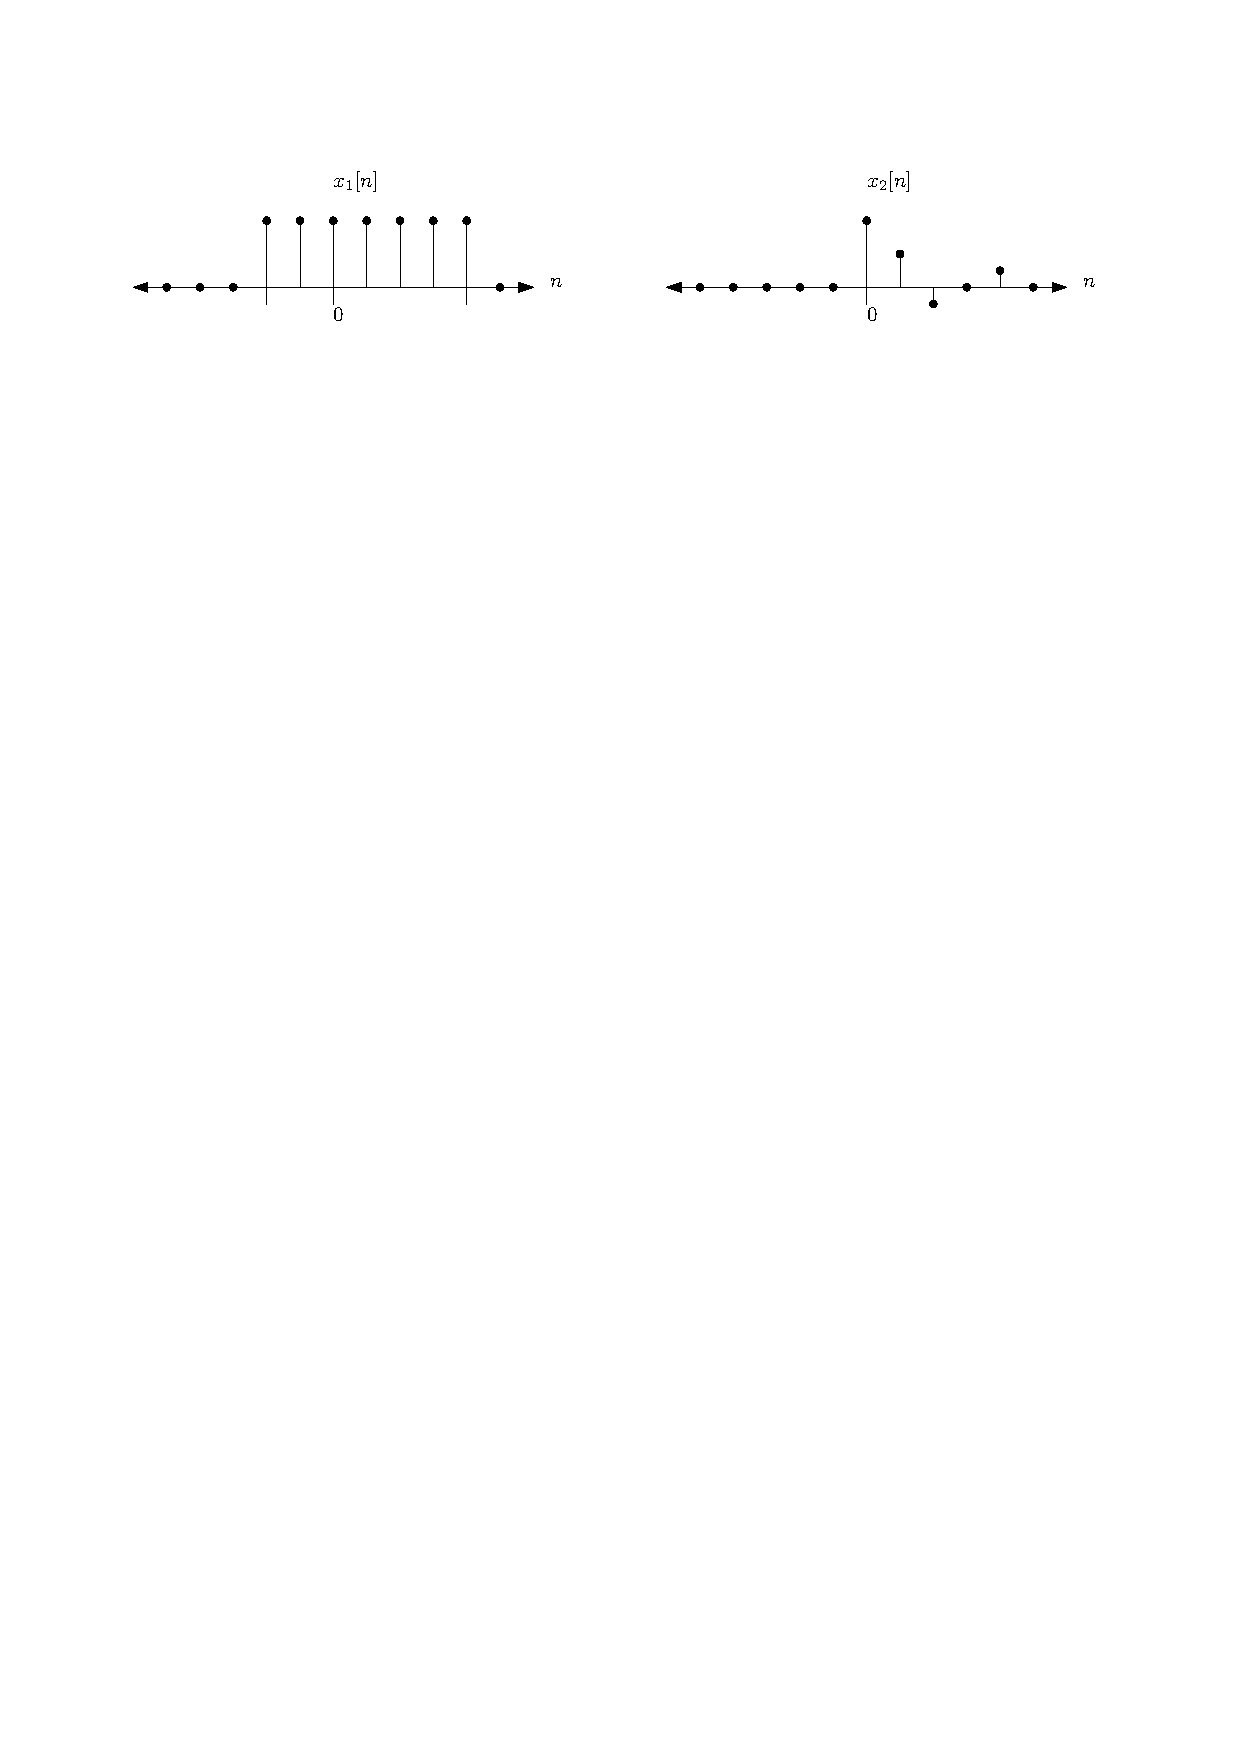
\includegraphics[scale=1]{graphics/dtconvolution-explain1.pdf}
\end{center}

Then $x_1[m]$ and $x_2[-m]$ look like
\begin{center}
  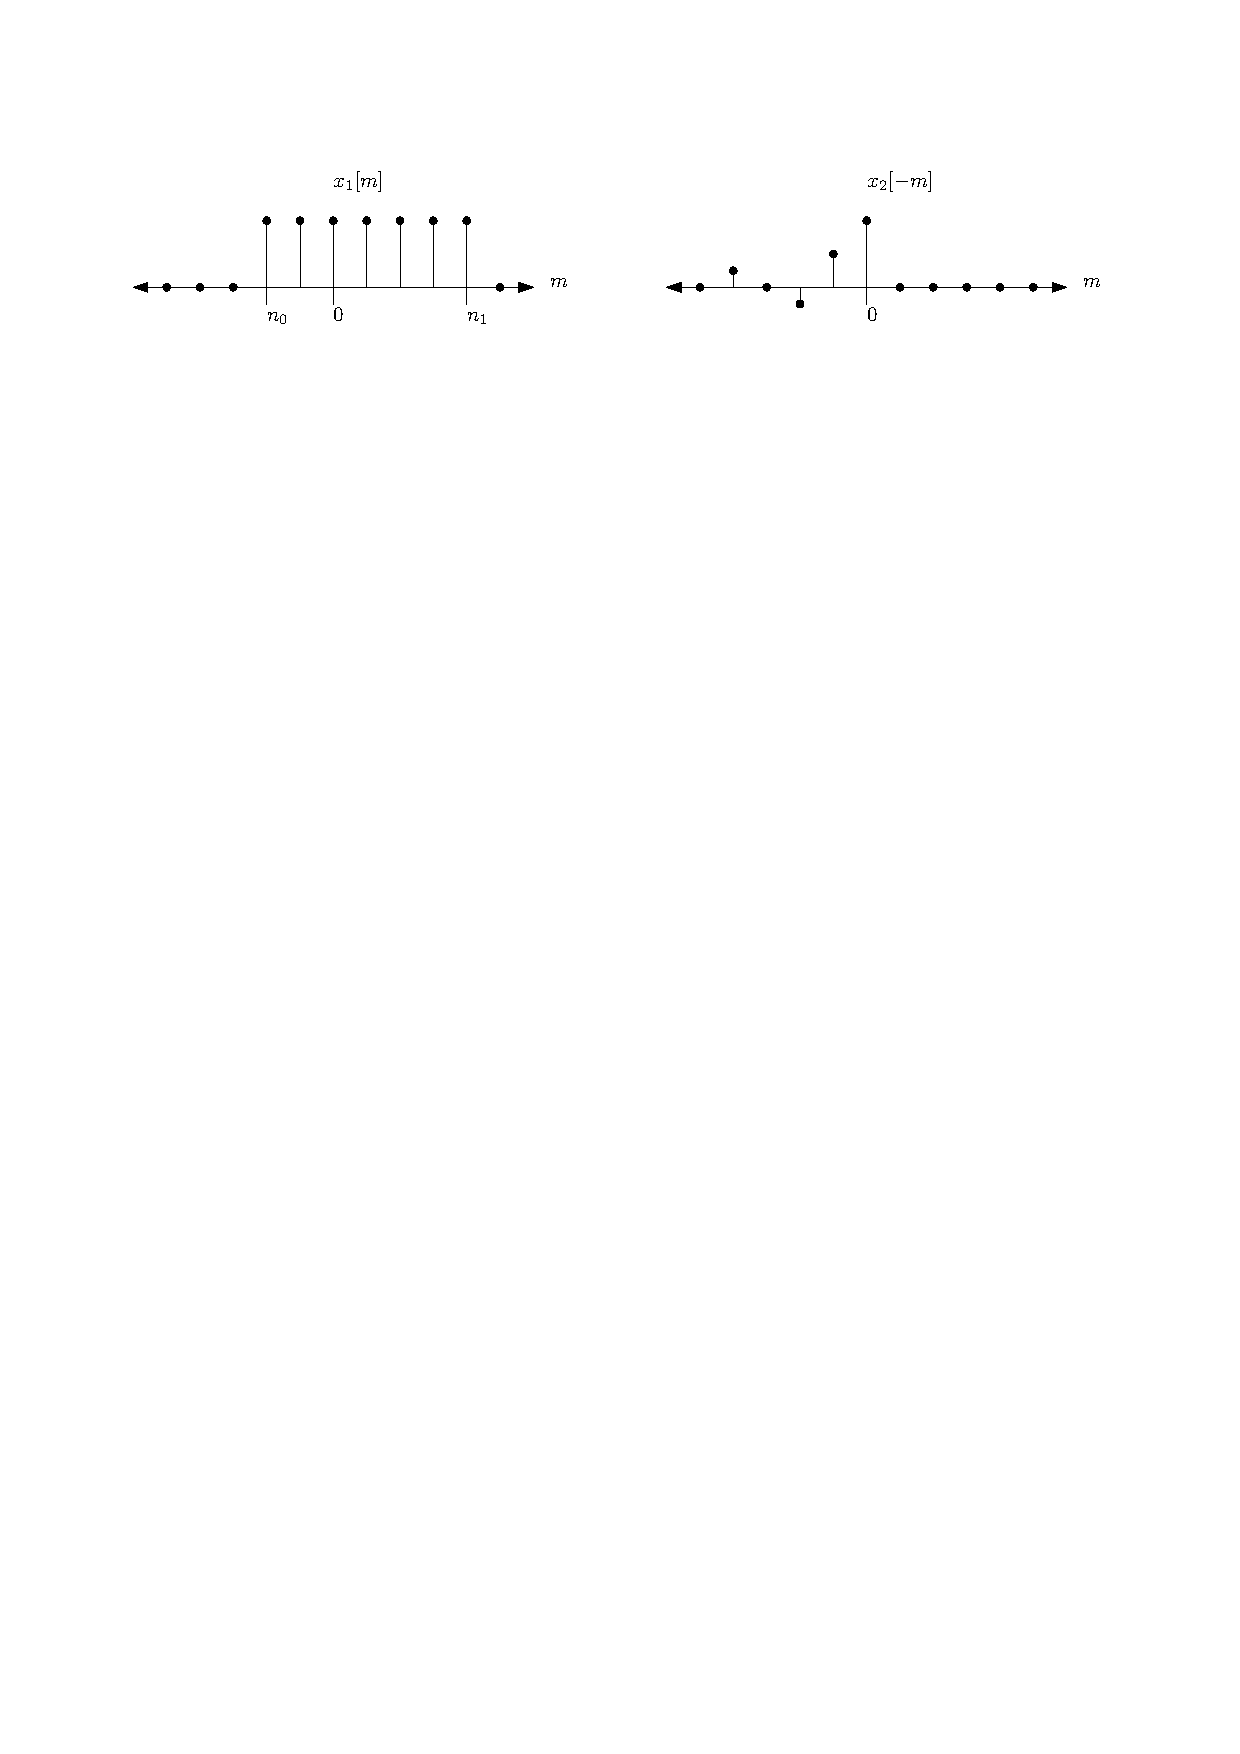
\includegraphics[scale=1]{graphics/dtconvolution-explain2.pdf}
\end{center}

The signal $x_2[n-m]$ is $x_2[-m]$ shifted by $n$ (since $x_2[-m+n]= x_s[n-m]$) and looks like
\begin{center}
  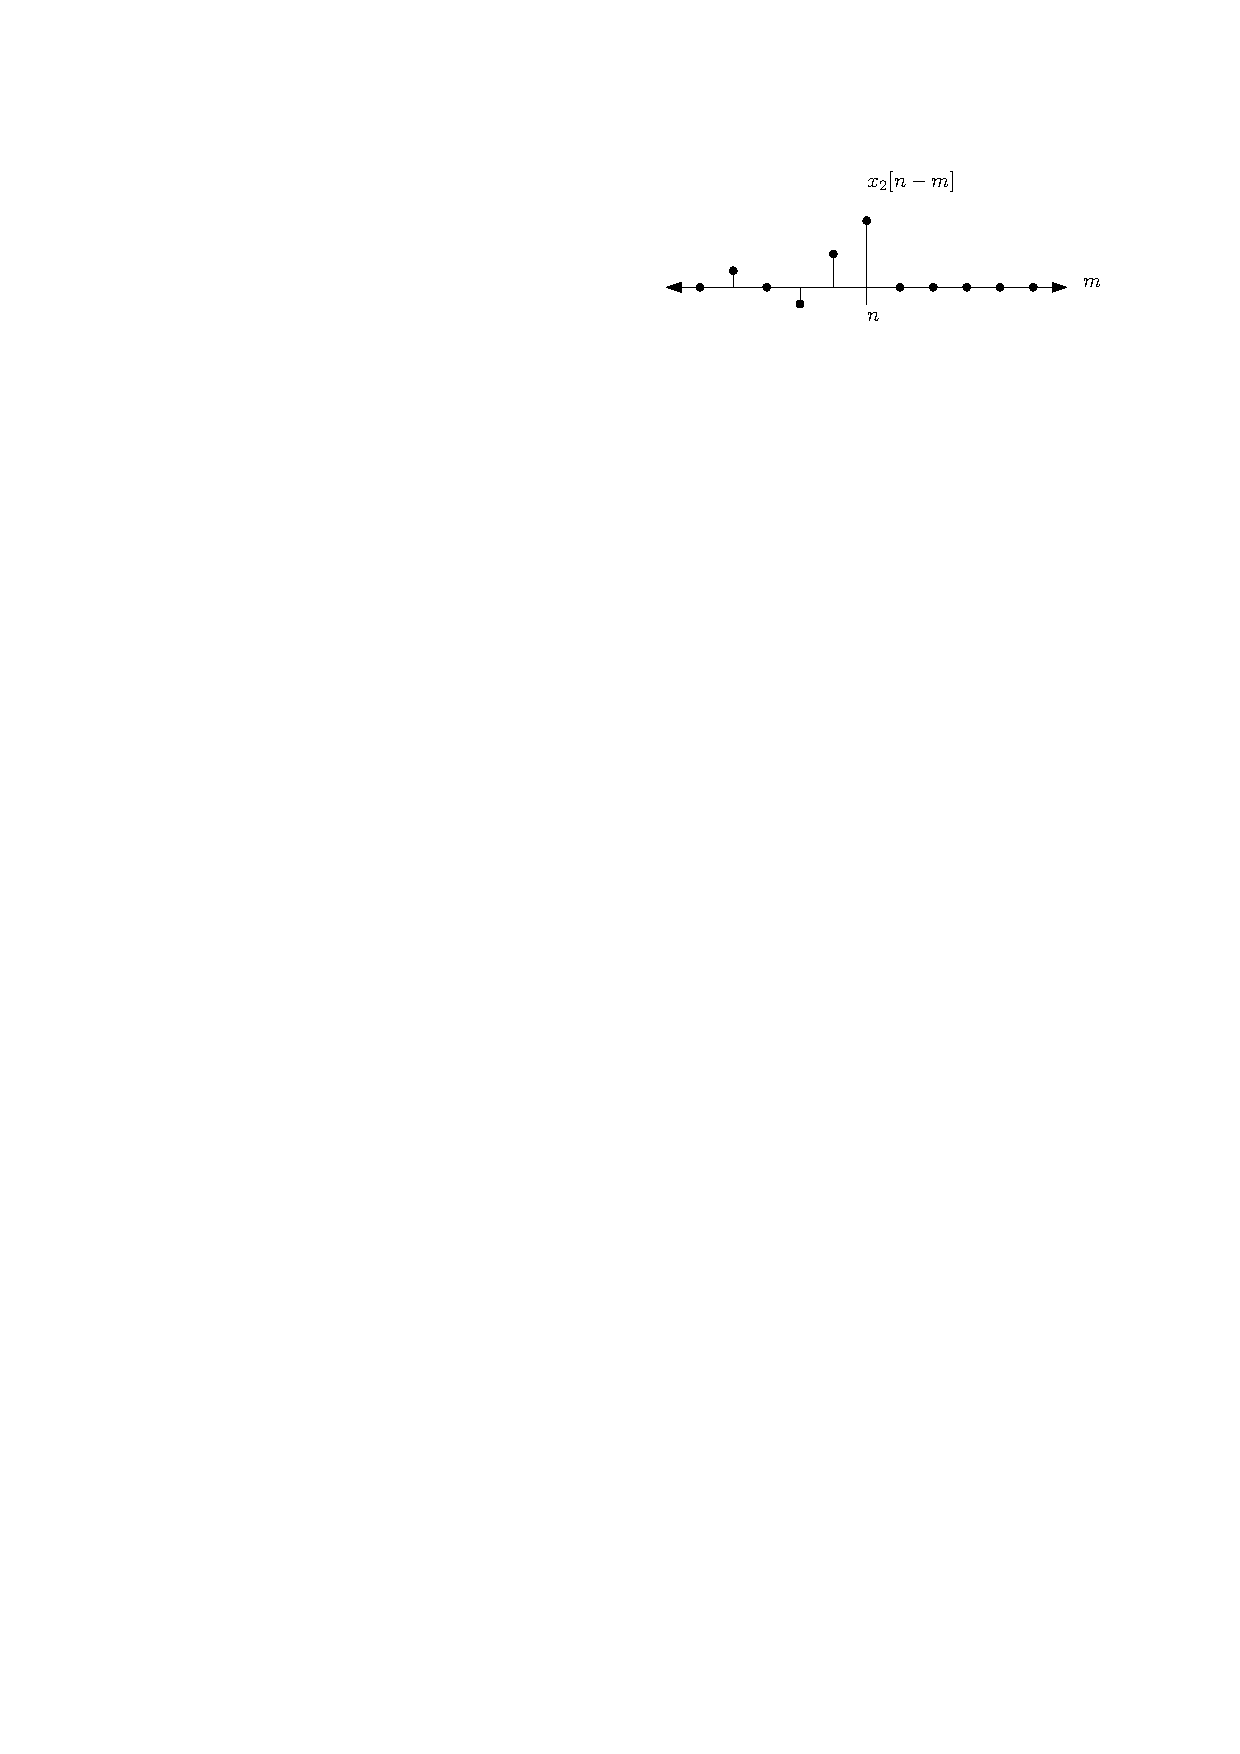
\includegraphics[scale=1]{graphics/dtconvolution-explain3.pdf}
\end{center}

Then the terms of the convolution sum is the product $x_1[m]x_2[n-m]$ whose plot depends of the value of $n$. Some examples, where the individual signals are in grey and their product is in bold:
\begin{center}
  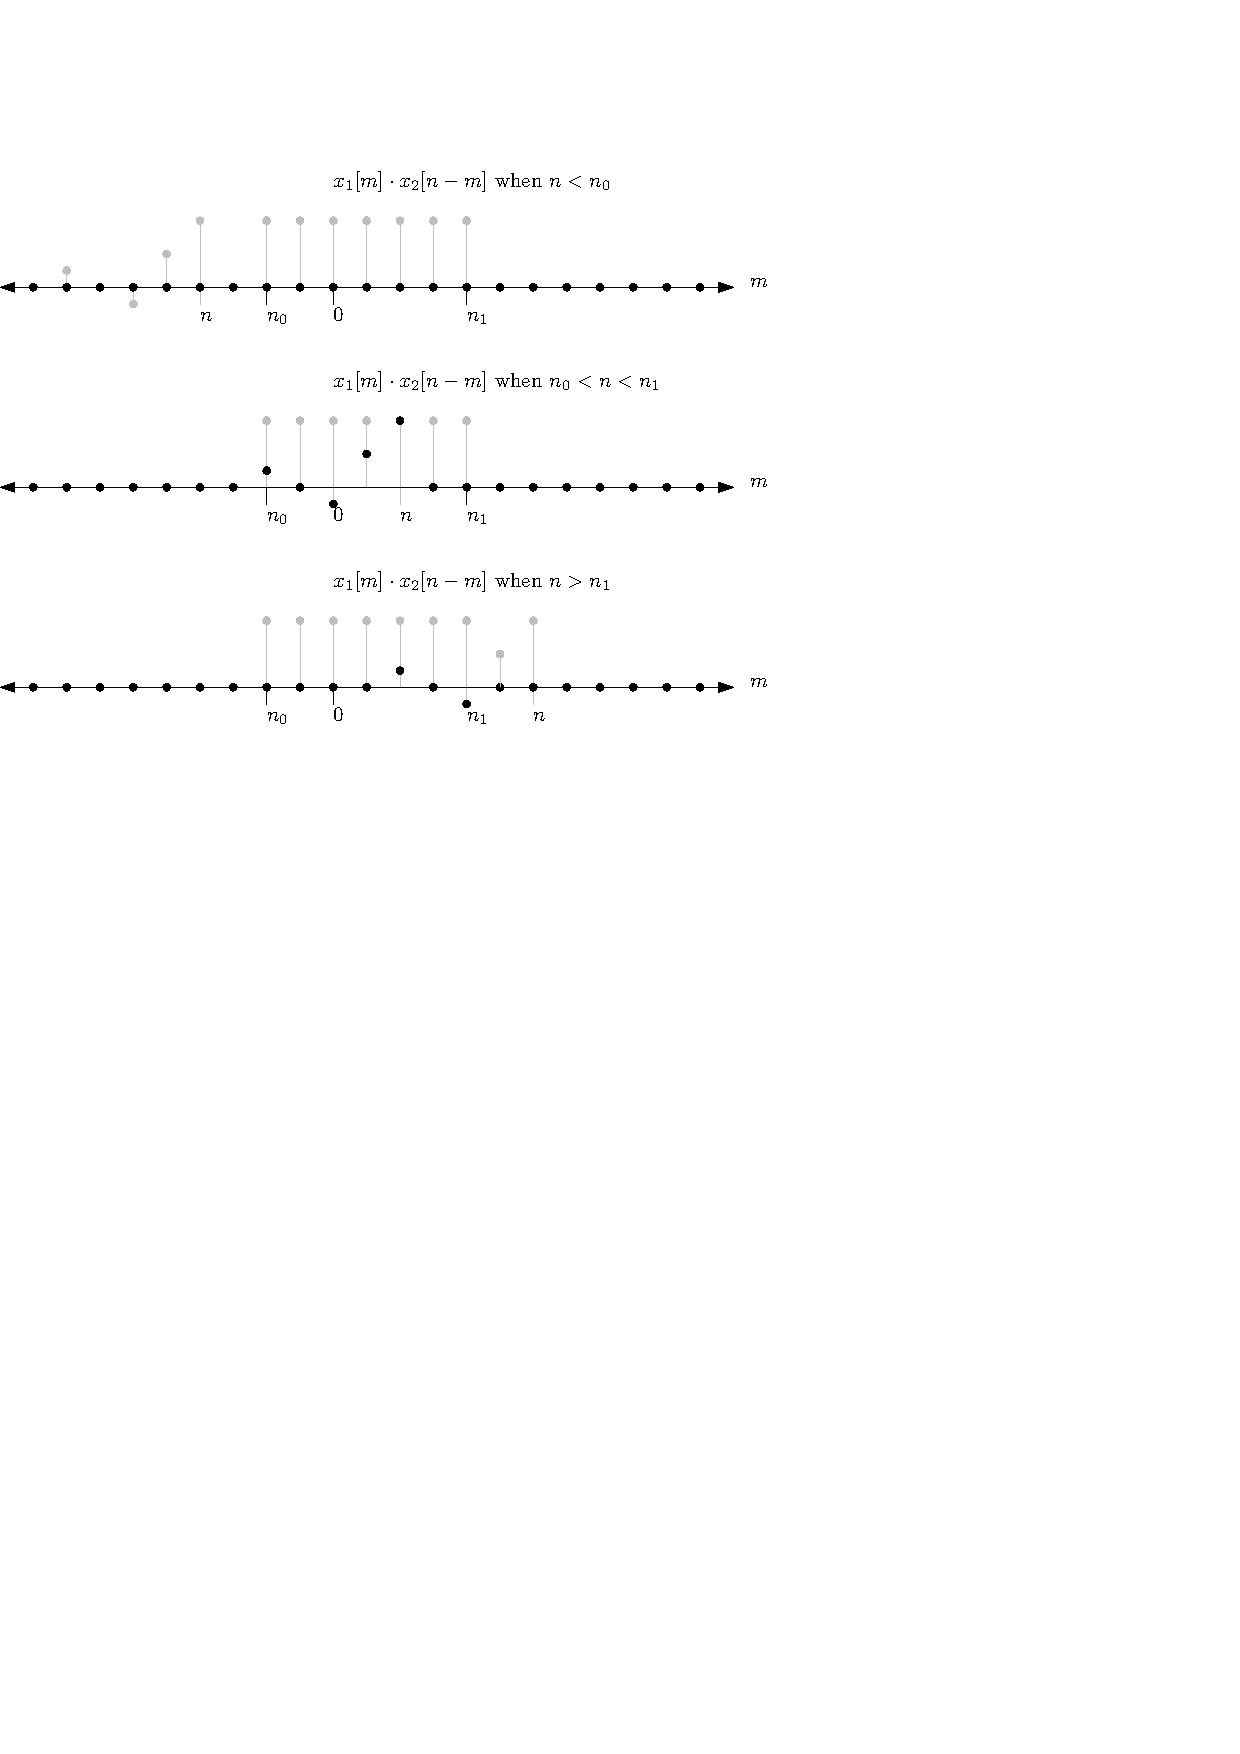
\includegraphics[scale=1]{graphics/dtconvolution-explain4.pdf}
\end{center}

Then convolution is the total sum of the product (bold plots above) for that value of $n$. For the example above we see the sum will be zero for $n$ less than $n_0$ since the two signals do not overlap and their product is zero. For $n_0 \leq n \leq n_1$ the signals overap and the product is non-zero, and the effective bounds of summation are $[n_0,n]$. For $n > n_1$ the signals again overap and the product is non-zero, but the effective bounds of summation are $[n_0,n_1]$. 

\section{DT Convolution of Finite-Length Signals}

For finite-length signals, DT convolution gives us an algorithm to determine their convolution. Suppose the signal $x_1$ is non-zero only over the interval $[N_1,M_1]$, and the signal $x_2$ is non-zero only over the interval $[N_2,M_2]$. The \emph{length} of the signals are $L_1 = M_1-N_1+1$ and $L_2 = M_2-N_2+1$ respectively. The non-zero terms of the convolution sum (when the signals overlap) is then the range $[N_1+N_2,M_1+M_2]$ and the sum can be truncated as:

\[
x_1[n] * x_2[n] = \sum\limits_{m = N_1+N_2}^{M_1+M_2} x_1[m]x_2[n-m]
\]

It is common to shift both signals so that they both start at index $0$ (in order to be represented as arrays in a zero-based index programming language like C or C++), zero-padding them both to have length $L=L_1+L_2-1$ (zero-pad means to just add zero values to the end of the sequence). Then the convolution becomes
\[
y = x_1 * x_2 = \sum\limits_{m = 0}^{L-1} x_1[m]x_2[n-m]
\]
where the indexing of $x_2$ is modulo the signal length, i.e. $x_2[(n-m) \mbox{ mod } L]$. The resulting signal after convolution, $y$, is also of length $L$, and can then be shifted back to start at $N_1+N_2$.

\begin{example} The following C++ code computes the convolution of the DT signals $\{1,-1,1\}$ and $\{1,1,1,1\}$.
\begin{verbatim}
  const unsigned int L = 6;
  double x1[L] = {1., -1., 1., 0, 0, 0};
  double x2[L] = {1., 1., 1., 1., 0, 0};
  double y[L];

  for(int n = 0; n < L; n++){
    double sum = 0.;
    for(int m = 0; m < L; m++){
      int idx = (L+n-m) % L;
      sum += x1[m]*x2[idx];
    }
    y[n] = sum;
  }
\end{verbatim}
Note that $L_1 = 3$, $L_2 = 4$, so that $L=6$.
$\blacksquare$
\end{example}

An interesting aside, convolution of finite length signals is equivalent to multiplication of two polynomials, where the signal values are the coefficients.

\section{Examples of DT Convolution}

\begin{example} Consider the convolution of two unit step functions:
  \[
  u[n] * u[n] = \sum\limits_{m = -\infty}^{\infty} u[m]u[n-m]
  \]
  Note for $n < 0$ the product of the signals $u[m]$ and $u[n-m]$ is zero as shown in the following figure
  \begin{center}
  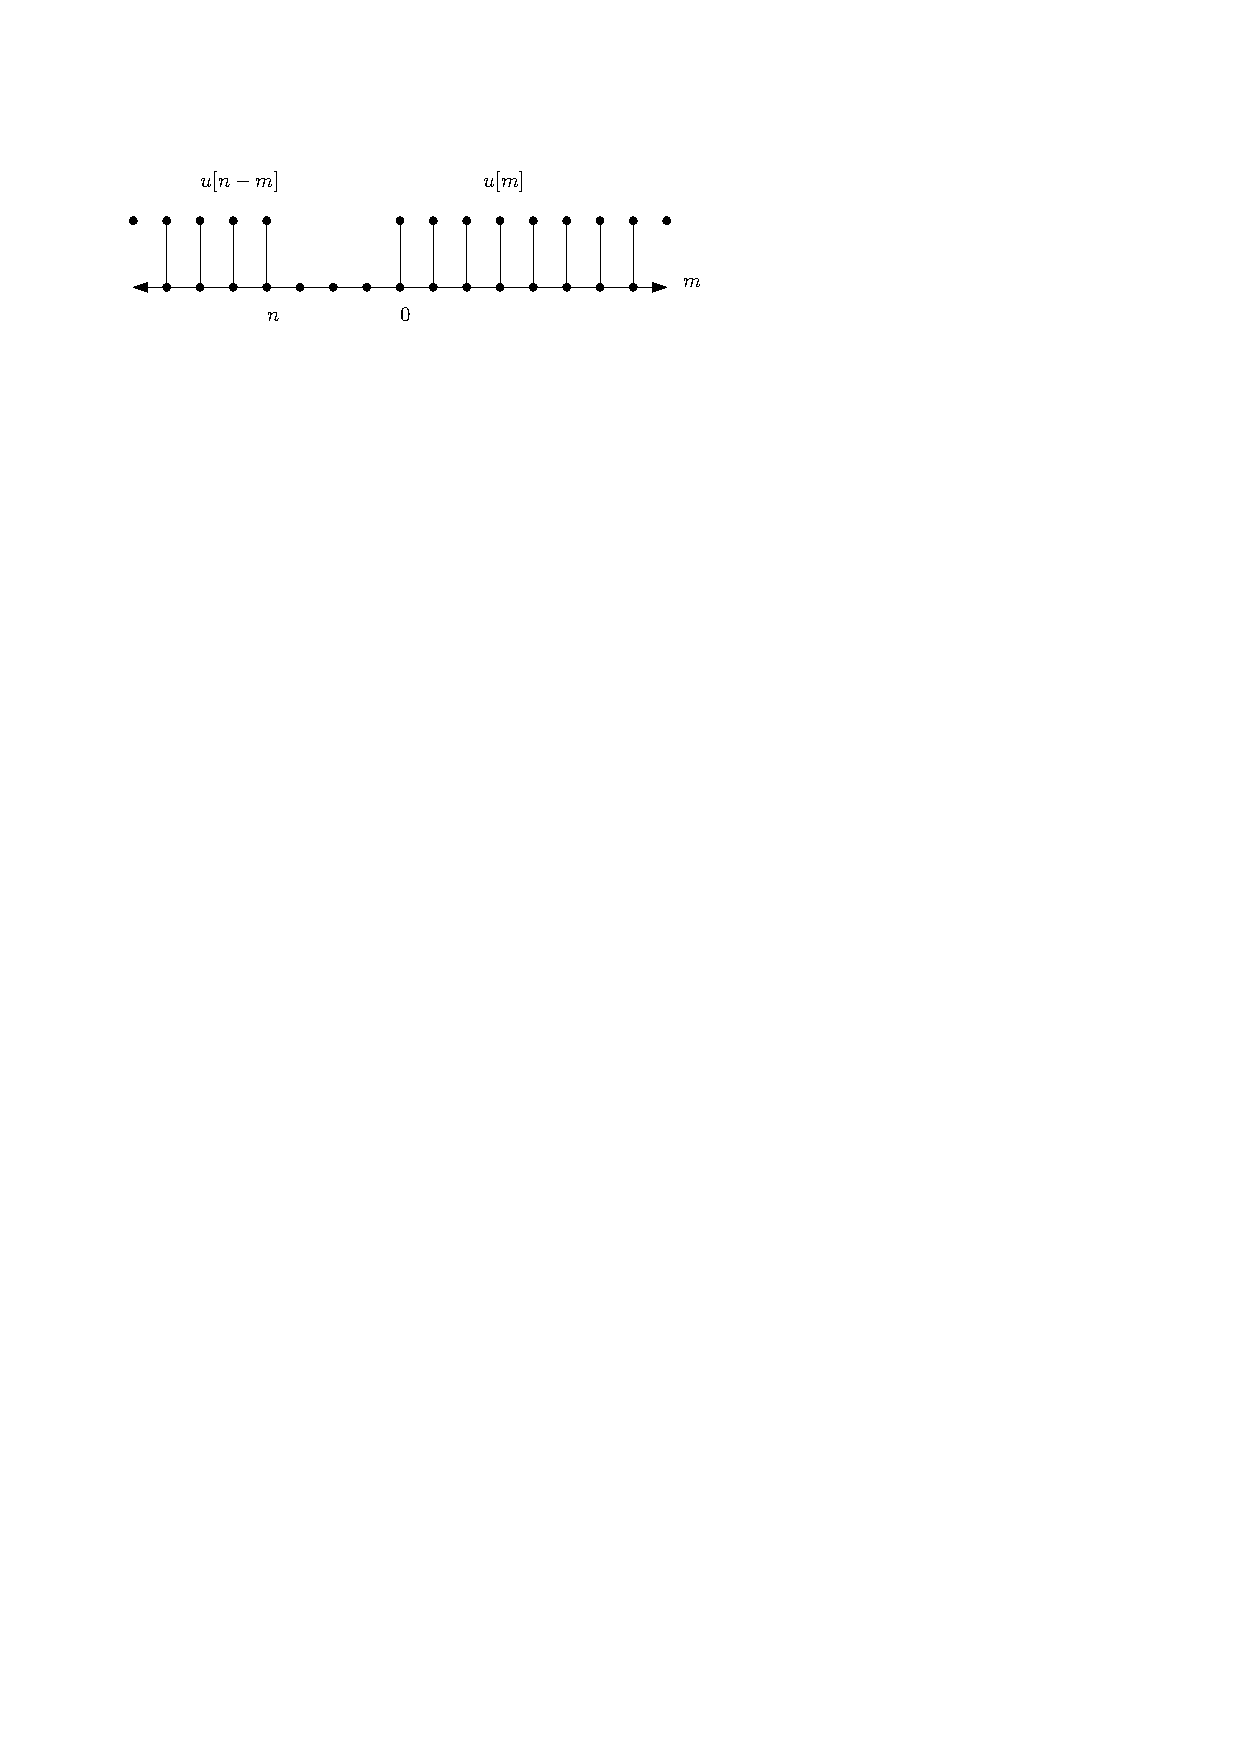
\includegraphics[scale=1]{graphics/dt-step-step-conv.pdf}
  \end{center}
  so that the resulting sum is zero for any $n < 0$. For $n \geq 0$ the signals $u[m]$ and $u[n-m]$ overlap from $0$ to $n$ as shown below
  \begin{center}
    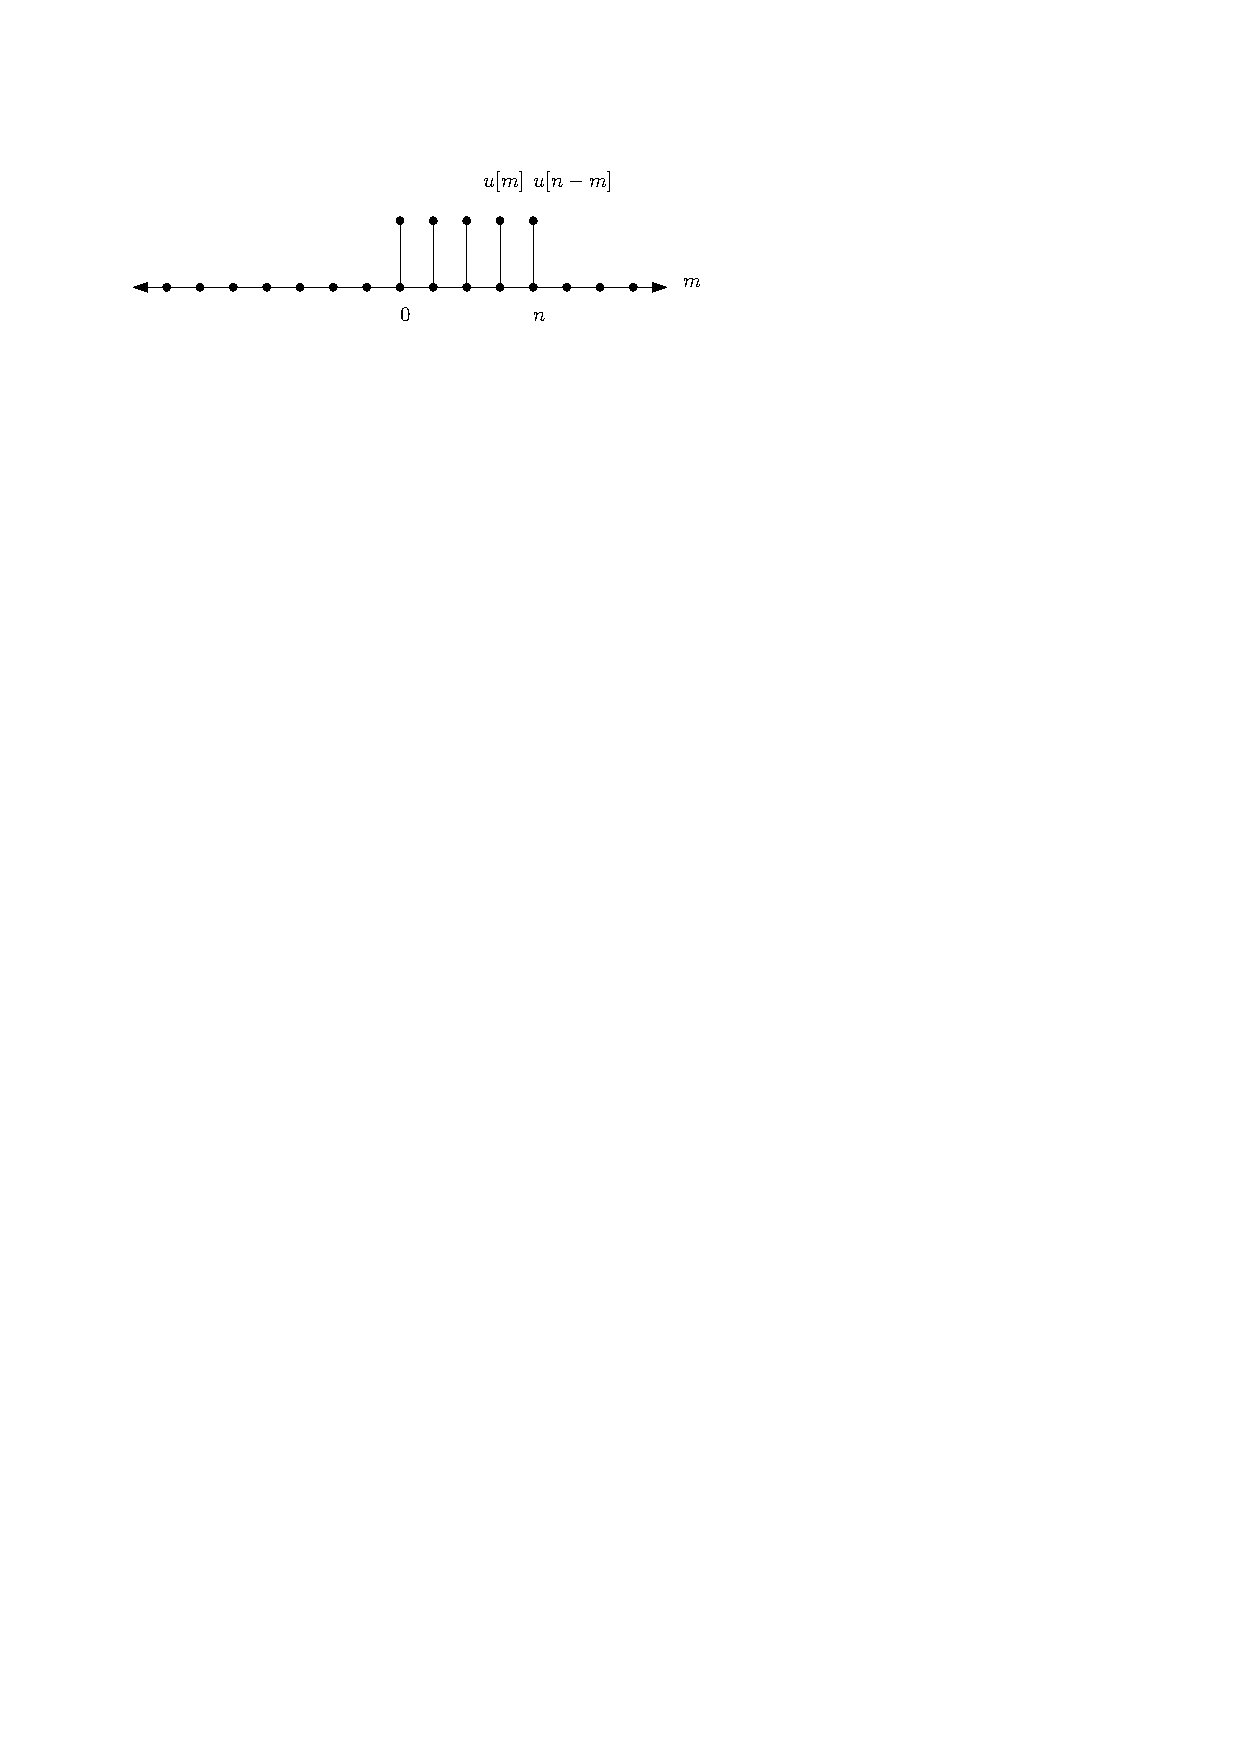
\includegraphics[scale=1]{graphics/dt-step-step-conv2.pdf}
  \end{center}
  and the convolution sum is
  \[
  \sum\limits_{m = 0}^{n} 1 = (n+1)
  \]
  so that
  \[
  u[n] * u[n] = \left\{ \begin{array}{lc}
    0 & n < 0\\
    n+1 & n \geq 0
  \end{array}
  \right.
  \]
  Putting the piecewise result into a single expression gives
  \[
  u[n] * u[n] = (n+1)u[n]
  \]
  $\blacksquare$
\end{example}

\begin{example}
Consider the convolution of a unit step and the function $\gamma^n\,u[n]$ for some constant $\gamma \neq 1$:
  \[
  \gamma^n\, u[n] * u[n] = \sum\limits_{m = -\infty}^{\infty} \gamma^{m}u[m]u[n-m]
  \]
  Since both signals are multiplied by a step, the product of $\gamma^{m}u[m]u[n-m]$ is non-zero only for $0 \leq m \leq n$ (for the same reason as in the previous example). Thus for $n \geq 0$ the convolution sum is:
  \[
  \sum\limits_{m = 0}^{n} \gamma^{m} = \frac{\gamma^{n+1}-1}{\gamma-1} = \frac{1-\gamma^{n+1}}{1-\gamma}
  \]
  Putting the two piecewise results together gives
  \[
  \gamma^n\, u[n] * u[n] = \frac{1-\gamma^{n+1}}{1-\gamma}\,u[n]
  \]
  $\blacksquare$
\end{example}
\begin{example} Consider the convolution of an arbitrary signal $x[n]$ with the impulse function
  \[
  x[n] * \delta[n] = \sum\limits_{m = -\infty}^{\infty} x[m]\delta[n-m]
  \]
  By the sifting property we get
  \[
  \sum\limits_{m = -\infty}^{\infty} x[m]\delta[n-m] = x[n]
  \]
  Thus the convolution with the impulse gives back the same signal (the $\delta$ is the \emph{identity} signal). $\blacksquare$
\end{example}

\noindent Table \ref{table:dtconv} lists several DT convolution results.

\section{Properties of DT Convolution}
There are several useful properties of convolution. We do not prove these here, but it is not terribly difficult to do so. Given signals $x_1[n]$, $x_2[n]$, and $x_3[n]$:

\begin{description}
\item [Commutative Property] The ordering of the signals does not matter.
  \[
x_1[n] * x_2[n] = x_2[n] * x_1[n]
  \]
\item [Distributive Propery] Convolution is distributed over addition.
  \[
  x_1[n] * \left(x_2[n] + x_3[n]\right) = \left(x_1[n] * x_2[n] \right) + \left(x_1[n] * x_3[n] \right) 
  \]
\item [Associative Property] The order of convolution does not matter.
    \[
  x_1[n] * \left(x_2[n] * x_3[n]\right) = \left(x_1[n] * x_2[n] \right) * x_3[n] 
  \]
\item [Index Shift] Given $x_3[n] = x_1[n] * x_2[n]$ then for index shifts $m_1, m_2 \in \mathbb{R}$
  \[
  x_1[n-m_1] * x_2[n-m_2] = x_3[n-m_1 - m_2]
  \]
\item [Multiplicative Scaling] Given $x_3[n] = x_1[n] * x_2[n]$ then for constants $a,b \in \mathbb{C}$
  \[
  \left(a\, x_1[n]\right) * \left(b\, x_2[n]\right) = a\, b\, x_3[n]
  \]
\end{description}

These properties can be used in combination with a table like that above to compute the convolution of a wide variety of signals without evaluating the summations.

\begin{example} Consider the convolution of the causal DT pulse of length $N$, $x_1[n] = u[n] - u[n-N]$, and the signal $x_2[n] = \left( \frac{1}{2}\right)^nu[n]$.

  \begin{align*}
    x_1[n] * x_2[n] &= \left( u[n] - u[n-N]\right) * \left( \left( \frac{1}{2}\right)^nu[n] \right)\\
    &= \left( u[n] \right) * \left( \left( \frac{1}{2}\right)^nu[n] \right) - \left( u[n-N]\right) * \left( \left( \frac{1}{2}\right)^nu[n] \right) \mbox{ using distributive property}\\
    &= \frac{1-\left(\frac{1}{2}\right)^{n+1}}{1-\left(\frac{1}{2}\right)}u[n] - \frac{1-\left(\frac{1}{2}\right)^{n+1}}{1-\left(\frac{1}{2}\right)}u[n] \Big|_{n\rightarrow n-N} \mbox{ from Table row 2 and index shift property}\\
    &= \frac{1-\left(\frac{1}{2}\right)^{n+1}}{\left(\frac{1}{2}\right)}u[n] - \frac{1-\left(\frac{1}{2}\right)^{n-N+1}}{\left(\frac{1}{2}\right)}u[n-N]\\
    &= \frac{1-\left(\frac{1}{2}\right)^{n+1}}{\left(\frac{1}{2}\right)}u[n] - \frac{1-\left(\frac{1}{2}\right)^{-N}\left(\frac{1}{2}\right)^{n+1}}{\left(\frac{1}{2}\right)}u[n-N]\\
    &= 2\left(1-\left(\frac{1}{2}\right)^{n+1}\right)u[n] - 2\left(1-\left(\frac{1}{2}\right)^{-N}\left(\frac{1}{2}\right)^{n+1} \right)u[n-N]\\
    &= \left(2-\left(\frac{1}{2}\right)^{n}\right)u[n] - \left(2-\left(\frac{1}{2}\right)^{-N}\left(\frac{1}{2}\right)^{n} \right)u[n-N]
  \end{align*}
$\blacksquare$
\end{example}


\newpage
\section{CT Block Diagrams}

\subsection{The Four Basic Motifs}

Understanding complex systems, with many interconnections, is aided by graphical representations, generally called block diagrams \footnote{There is a closely related graphical approach called \emph{signal flow graphs} that you may learn about in upper-level courses. They are equivalent to block diagrams, but are more amenable to computer representation and manipulation.}. They are a hybrid graphical-analytical approach.

There are just four basic motifs needed to build any block diagram. Let $\mathcal{S}_i$ denote a (sub) system. Then the four motifs are:

\begin{itemize}
\item A single block.\\[1em] 
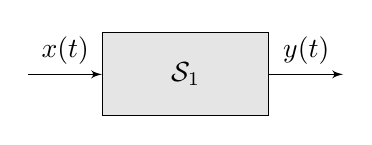
\begin{tikzpicture}[auto, node distance=2cm,>=latex',scale=1, every node/.style={transform shape}]
    % We start by placing the blocks
    \node [input, name=input] {};
    \node [block, right of=input] (system) {$\mathcal{S}_1$};
    \node [output, right of=system] (output) {};

    % Once the nodes are placed, connecting them is easy. 
    \draw [draw,->] (input) -- node {$x(t)$} (system);
    \draw [->] (system) -- node {$y(t)$} (output);
\end{tikzpicture}

\item A {\it series} connection of two blocks\\[1em]
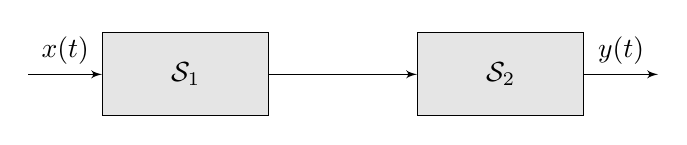
\begin{tikzpicture}[auto, node distance=2cm,>=latex',scale=1, every node/.style={transform shape}]
    % We start by placing the blocks
    \node [input, name=input] {};
    \node [block, right of=input] (system1) {$\mathcal{S}_1$};
    \node [block, right of=system1,node distance=4cm] (system2) {$\mathcal{S}_2$};
    \node [output, right of=system2] (output) {};

    % Once the nodes are placed, connecting them is easy. 
    \draw [draw,->] (input) -- node {$x(t)$} (system1);
    \draw [->] (system1) -- (system2);
    \draw [->] (system2) -- node {$y(t)$} (output);
\end{tikzpicture}
\item A {\it parallel} connection of two blocks\\[1em]
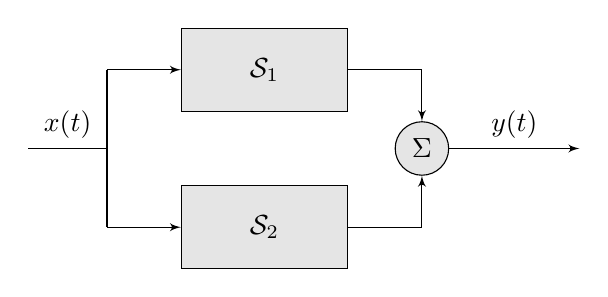
\begin{tikzpicture}[auto, node distance=2cm,>=latex',scale=1, every node/.style={transform shape}]
    % We start by placing the blocks and inputs
    \node[shape=coordinate] at (1,1) (input1) {};
    \node[block] at (3,1) (block1) {$\mathcal{S}_1$};
    \node[shape=coordinate] at ($(block1.east)+(0.5,0)$) (output1) {};
    \draw[->] (input1) -- (block1);
    \draw (block1) -- (output1);

    \node[shape=coordinate] at (1,-1) (input2) {};
    \node[block] at (3,-1) (block2) {$\mathcal{S}_2$};
    \node[shape=coordinate] at ($(block2.east)+(0.5,0)$) (output2) {};
    \draw[->] (input2) -- (block2);
    \draw (block2) -- (output2);

    \node [input, name=input] at (0,0) {};  	
    \node [input, name=conn] at (1,0) {};
    \draw (conn) -- (input1);
    \draw (conn) -- (input2);
    \node [sum, right of=input,node distance=5cm] (sum) {$\Sigma$};
    \draw [->] (output1) -| (sum);
    \draw [->] (output2) -| (sum);

    \draw [draw] (input) -- node {$x(t)$} (conn);
    \node [output, right of=sum] (output) {};
    \draw [->] (sum) -- node {$y(t)$} (output);
\end{tikzpicture}

\item A {\it feedback} connection\\[1em]
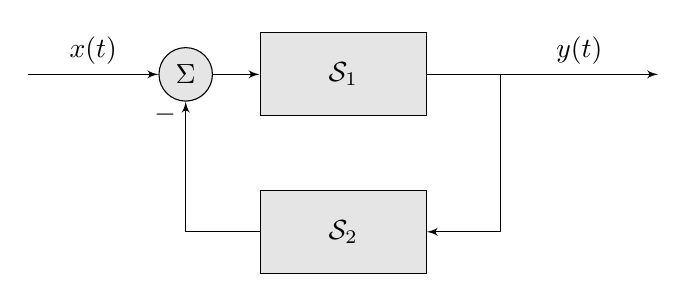
\begin{tikzpicture}[auto, node distance=2cm,>=latex',scale=1, every node/.style={transform shape}]
    % We start by placing the blocks
    \node[block] at (4,0) (block1) {$\mathcal{S}_1$};

    \node[block] at (4,-2) (block2) {$\mathcal{S}_2$};
    \node[shape=coordinate] at (6,-2) (input2) {};

    \node [input, name=input] at (0,0) {};  	
    \node [shape=coordinate, name=conn] at (6,0) {};
    \draw (block1) -- (conn);
    \draw (conn) -- (input2);
    \draw [->] (input2) -- (block2);

    \node [sum, right of=input,node distance=2cm] (sum) {$\Sigma$};
    \draw [->] (block2) -| node[pos=0.95] {$-$} (sum);

    \draw [draw,->] (input) -- node {$x(t)$} (sum);
    \draw [->] (sum) -- (block1);
    \node [output, right of=conn] (output) {};
    \draw [->] (conn) -- node {$y(t)$} (output);
\end{tikzpicture}
\end{itemize}

Note the feedback is negative (the minus sign on the feedback summation input). These can be use in various combinations, as we shall see shortly.

\subsection{Connections to Convolution}

Each subsystem, $\mathcal{S}_i$, can be represented by a basic time-domain operation (e.g. derivatives, integrals, addition, and scaling) or more generally by it's impulse response $h_i(t)$.
\
For example a block representing an system acting as integrator is typically drawn as

\begin{center}
  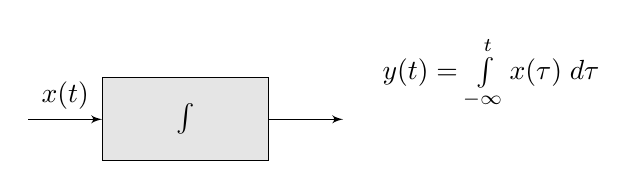
\begin{tikzpicture}[auto, node distance=2cm,>=latex',scale=1, every node/.style={transform shape}]
    % We start by placing the blocks
    \node [input, name=input] {};
    \node [block, right of=input] (system) {$\int$};
    \node [output, right of=system] (output) {};

    % Once the nodes are placed, connecting them is easy. 
    \draw [draw,->] (input) -- node {$x(t)$} (system);
    \draw [->] (system) -- node[pos=3] {$y(t) = \int\limits_{-\infty}^t x(\tau) \; d\tau$} (output);
\end{tikzpicture}
\end{center}
This is equivalent to an impulse response $h(t) = u(t)$ so that it might also be drawn as
\begin{center}
  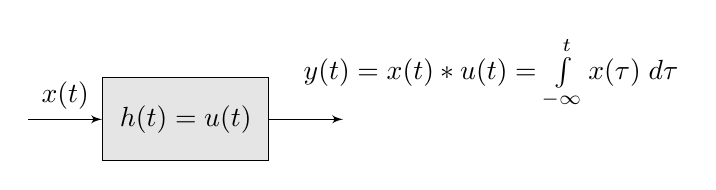
\begin{tikzpicture}[auto, node distance=2cm,>=latex',scale=1, every node/.style={transform shape}]
    % We start by placing the blocks
    \node [input, name=input] {};
    \node [block, right of=input] (system) {$h(t) = u(t)$};
    \node [output, right of=system] (output) {};

    % Once the nodes are placed, connecting them is easy. 
    \draw [draw,->] (input) -- node {$x(t)$} (system);
    \draw [->] (system) -- node[pos=3] {$y(t) = x(t) * u(t) = \int\limits_{-\infty}^t x(\tau) \; d\tau$} (output);
\end{tikzpicture}
\end{center}

We can use the concept of convolution to connect block diagrams to the properties of convolution

\begin{itemize}
\item A single block is equivalent to convolution with the impulse response for that subsystem\\[1em] 
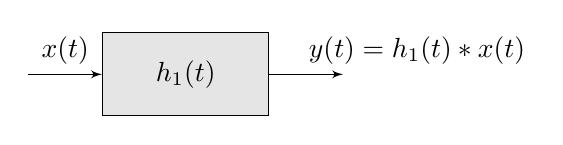
\begin{tikzpicture}[auto, node distance=2cm,>=latex',scale=1, every node/.style={transform shape}]
    % We start by placing the blocks
    \node [input, name=input] {};
    \node [block, right of=input] (system) {$h_1(t)$};
    \node [output, right of=system] (output) {};

    % Once the nodes are placed, connecting them is easy. 
    \draw [draw,->] (input) -- node {$x(t)$} (system);
    \draw [->] (system) -- node[pos=2] {$y(t) = h_1(t)*x(t)$} (output);
\end{tikzpicture}

\item Using the associative property, a series connection of two blocks becomes
  \begin{center}
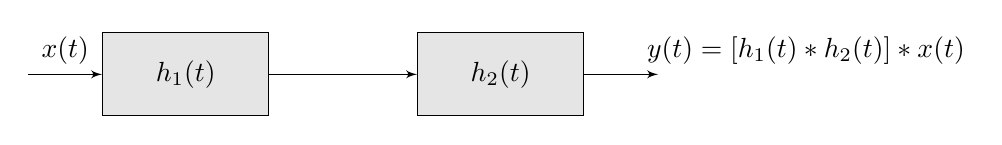
\begin{tikzpicture}[auto, node distance=2cm,>=latex',scale=1, every node/.style={transform shape}]
    % We start by placing the blocks
    \node [input, name=input] {};
    \node [block, right of=input] (system1) {$h_1(t)$};
    \node [block, right of=system1,node distance=4cm] (system2) {$h_2(t)$};
    \node [output, right of=system2] (output) {};

    \draw [draw,->] (input) -- node {$x(t)$} (system1);
    \draw [->] (system1) -- (system2);
    \draw [->] (system2) -- node[pos=3] {$y(t) = \left[h_1(t)*h_2(t)\right]*x(t)$} (output);
\end{tikzpicture}
  \end{center}
  which can be reduced to a single convolution $y(t) = h_3(t)*x(t)$ where $h_3(t) = h_1(t)*h_2(t)$.
\item Using the distributive property, a parallel connection of two blocks becomes
  \begin{center}
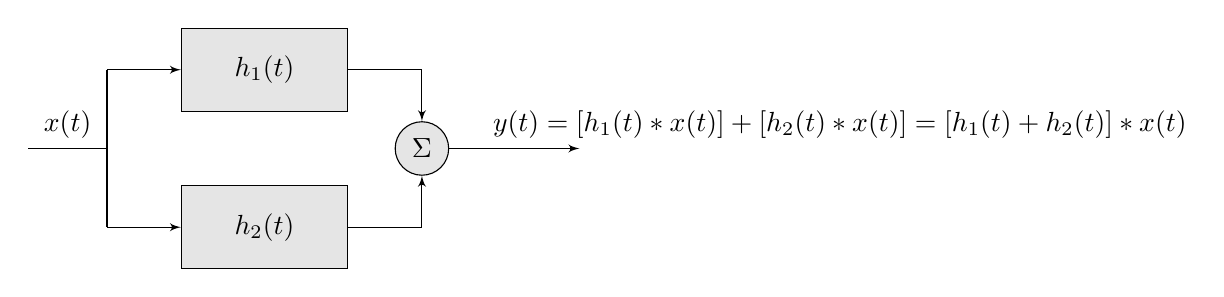
\begin{tikzpicture}[auto, node distance=2cm,>=latex',scale=1, every node/.style={transform shape}]

    \node[shape=coordinate] at (1,1) (input1) {};
    \node[block] at (3,1) (block1) {$h_1(t)$};
    \node[shape=coordinate] at ($(block1.east)+(0.5,0)$) (output1) {};
    \draw[->] (input1) -- (block1);
    \draw (block1) -- (output1);

    \node[shape=coordinate] at (1,-1) (input2) {};
    \node[block] at (3,-1) (block2) {$h_2(t)$};
    \node[shape=coordinate] at ($(block2.east)+(0.5,0)$) (output2) {};
    \draw[->] (input2) -- (block2);
    \draw (block2) -- (output2);

    \node [input, name=input] at (0,0) {};  	
    \node [input, name=conn] at (1,0) {};
    \draw (conn) -- (input1);
    \draw (conn) -- (input2);
    \node [sum, right of=input,node distance=5cm] (sum) {$\Sigma$};
    \draw [->] (output1) -| (sum);
    \draw [->] (output2) -| (sum);

    \draw [draw] (input) -- node {$x(t)$} (conn);
    \node [output, right of=sum] (output) {};
    \draw [->] (sum) -- node[pos=3] {$y(t)= \left[h_1(t)*x(t)\right] +  \left[h_2(t)*x(t)\right] =  \left[h_1(t)+h_2(t)\right]*x(t)$} (output);
\end{tikzpicture}  
  \end{center}
  which is equivalent to a single convolution $y(t) = h_3(t)*x(t)$ where $h_3(t) = h_1(t) + h_2(t)$.
\item In the feedback connection let $w(t)$ be the output of the summation
  \begin{center}
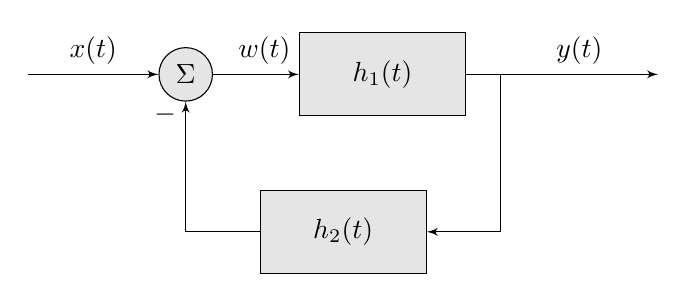
\begin{tikzpicture}[auto, node distance=2cm,>=latex',scale=1, every node/.style={transform shape}]
    % We start by placing the blocks
    \node[block] at (4.5,0) (block1) {$h_1(t)$};

    \node[block] at (4,-2) (block2) {$h_2(t)$};
    \node[shape=coordinate] at (6,-2) (input2) {};

    \node [input, name=input] at (0,0) {};  	
    \node [shape=coordinate, name=conn] at (6,0) {};
    \draw (block1) -- (conn);
    \draw (conn) -- (input2);
    \draw [->] (input2) -- (block2);

    \node [sum, right of=input,node distance=2cm] (sum) {$\Sigma$};
    \draw [->] (block2) -| node[pos=0.95] {$-$} (sum);

    \draw [draw,->] (input) -- node {$x(t)$} (sum);
    \draw [->] (sum) -- (block1);
    \node [output, right of=conn] (output) {};
    \draw [->] (conn) -- node {$y(t)$} (output);
    \draw node at (3,0.3) {$w(t)$};
\end{tikzpicture}
  \end{center}
  Then $y(t) = h_1(t)*w(t)$ and $w(t) = x(t) - h_2(t)*y(t)$. Substituting the later into the former gives $y(t) = h_1*(x-h_2(t)*y(t))$. Using the distributive property we get $y(t) = h_1(t)*x(t) - h_1(t)*h_2(t)*y(t)$. Isolating the input on the right-hand side and using $y(t) = \delta(t)*y(t)$ we get
  \[
  y(t) + h_1(t)*h_2(t)*y(t) = \left[\delta(t) + h_1(t)*h_2(t)\right]*y(t) = h_1(t)*x(t) 
  \]
  We can solve this for $y(t)$ using the concept of inverse systems. Let $h_3(t)* \left[\delta(t) + h_1(t)*h_2(t)\right]= \delta(t)$, i.e. $h_3$ is the inverse system of $\delta(t) + h_1(t)*h_2(t)$. Then
  \[
  y(t) = h_3(t)*h_1(t)*x(t)
  \]
\end{itemize}

Recall, when the system is instantaneous (memoryless) the impulse response is $a\delta(t)$ for some constant $a$. This is the same as scaling the signal by $a$. We typically drop the block in such cases and draw the input-output operation as

\begin{center}
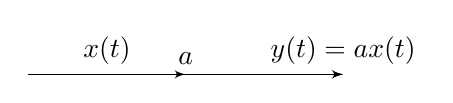
\begin{tikzpicture}[auto, node distance=2cm,>=latex',scale=1, every node/.style={transform shape}]
  \node [input, name=input] at (0,0) {};
  \node [output, name=system] at (2,0) {};
  \node [output, name=output] at (4,0) {};
  \draw [draw,->] (input) -- node {$x(t)$} (system);
  \draw [draw,->] (system) -- node[pos=1] {$y(t) = ax(t)$} (output);
  \draw [->] (input) -- node {$a$} (output);
\end{tikzpicture}
\end{center}

These properties allow us to perform transformations, either breaking up a system into subsystems, or reducing a system to a single block.

\begin{example}
  Consider a second-order system system with impulse response
  \[
  h(t) = \left(e^{-3t} - e^{-t}\right)\, u(t)
  \]
  We can express this as a block diagram consisting of two parallel blocks
  \begin{center}
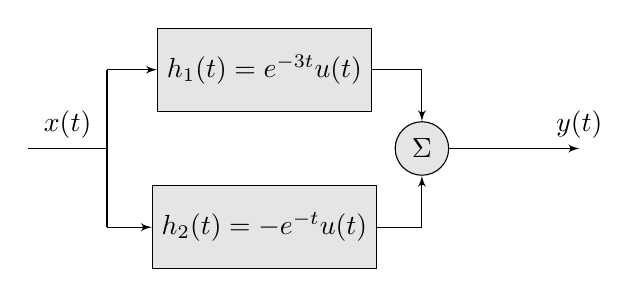
\begin{tikzpicture}[auto, node distance=2cm,>=latex',scale=1, every node/.style={transform shape}]

    \node[shape=coordinate] at (1,1) (input1) {};
    \node[block] at (3,1) (block1) {$h_1(t) = e^{-3t}u(t)$};
    \node[shape=coordinate] at ($(block1.east)+(0.5,0)$) (output1) {};
    \draw[->] (input1) -- (block1);
    \draw (block1) -- (output1);

    \node[shape=coordinate] at (1,-1) (input2) {};
    \node[block] at (3,-1) (block2) {$h_2(t) = -e^{-t}u(t)$};
    \node[shape=coordinate] at ($(block2.east)+(0.5,0)$) (output2) {};
    \draw[->] (input2) -- (block2);
    \draw (block2) -- (output2);

    \node [input, name=input] at (0,0) {};  	
    \node [input, name=conn] at (1,0) {};
    \draw (conn) -- (input1);
    \draw (conn) -- (input2);
    \node [sum, right of=input,node distance=5cm] (sum) {$\Sigma$};
    \draw [->] (output1) -| (sum);
    \draw [->] (output2) -| (sum);

    \draw [draw] (input) -- node {$x(t)$} (conn);
    \node [output, right of=sum] (output) {};
    \draw [->] (sum) -- node[pos=1] {$y(t)$} (output);
\end{tikzpicture}
  \end{center}

\end{example}

\begin{example}
  Consider a system with block diagram

  \begin{center}
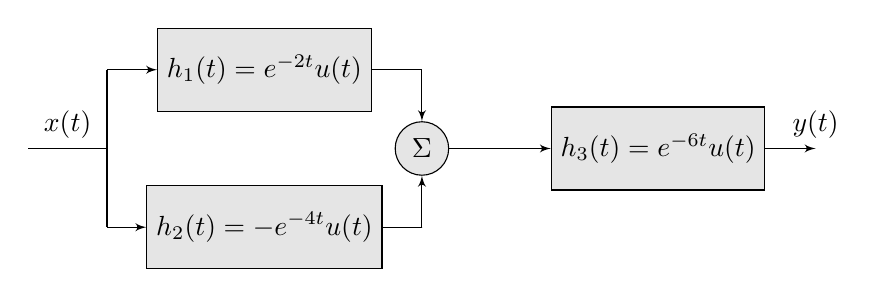
\begin{tikzpicture}[auto, node distance=2cm,>=latex',scale=1, every node/.style={transform shape}]

    \node[shape=coordinate] at (1,1) (input1) {};
    \node[block] at (3,1) (block1) {$h_1(t) = e^{-2t}u(t)$};
    \node[shape=coordinate] at ($(block1.east)+(0.5,0)$) (output1) {};
    \draw[->] (input1) -- (block1);
    \draw (block1) -- (output1);

    \node[shape=coordinate] at (1,-1) (input2) {};
    \node[block] at (3,-1) (block2) {$h_2(t) = -e^{-4t}u(t)$};
    \node[shape=coordinate] at ($(block2.east)+(0.5,0)$) (output2) {};
    \draw[->] (input2) -- (block2);
    \draw (block2) -- (output2);

    \node[block] at (8,0) (block3) {$h_3(t) = e^{-6t}u(t)$};

    \node [input, name=input] at (0,0) {};  	
    \node [input, name=conn] at (1,0) {};
    \draw (conn) -- (input1);
    \draw (conn) -- (input2);
    \node [sum, right of=input,node distance=5cm] (sum) {$\Sigma$};
    \draw [->] (output1) -| (sum);
    \draw [->] (output2) -| (sum);

    \draw [draw] (input) -- node {$x(t)$} (conn);
    \node [output, right of=block3] (output) {};
    \draw [->] (sum) -- (block3);
    \draw [->] (block3) -- node[pos=1] {$y(t)$} (output);
\end{tikzpicture}
  \end{center}
  We can determine the overall impulse response of this system using the distributive and associative properties
\begin{align*}
  h(t) &= \left[ h_1(t) + h_2(t)\right]*h_3(t)\\
  &= h_1(t)*h_3(t) + h_2(t)*h_3(t)\\
  &= \left[ e^{-2t}u(t)\right]*\left[ e^{-6t}u(t)\right] + \left[-e^{-4t}u(t) \right]*\left[ e^{-6t}u(t)\right]
\end{align*}
Using the convolution table from Lecture 8 we get the overall impulse response
\[
h(t) = \frac{e^{-2 t}-e^{-6 t}}{4}u(t) - \frac{e^{-4 t}-e^{-6 t}}{2}u(t) = \frac{1}{4}e^{-2t}u(t) -\frac{1}{2}e^{-4t}u(t) + \frac{1}{4}e^{-6t}u(t)
\]
\end{example}


\subsection{Connections to LCCDE}

The other system representation we have seen are linear, constant-coefficient differential equations. These can be expressed as combinations of derivative and/or integration blocks.

\subsubsection*{First-Order System}

To illustrate this consider the first-order LCCDE
\[
\frac{dy}{dt}(t) + ay(t) = x(t)
\]
We can solve this for $y(t)$
\[
y(t) = -\frac{1}{a} \frac{dy}{dt}(t) + \frac{1}{a}x(t)
\]
and can express this as a feedback motif
\begin{center}
  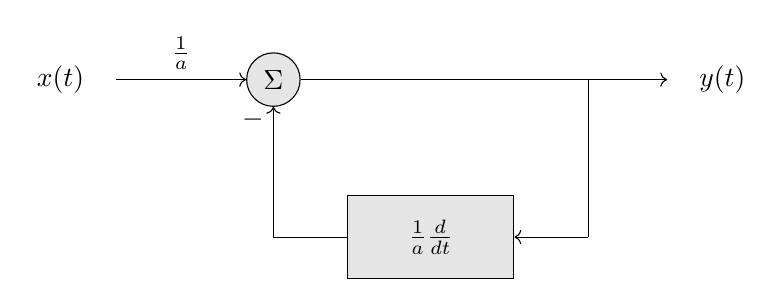
\begin{tikzpicture}[auto]
    \node[block] at (4,-2) (block2) {$\frac{1}{a}\frac{d}{dt}$};
    \node[shape=coordinate] at (6,-2) (input2) {};
    \node [input, name=input] at (0,0) {};  	
    \node [shape=coordinate, name=conn] at (6,0) {};
    \node [sum, right of=input,node distance=2cm] (sum) {$\Sigma$};
    
    \draw (sum) -- (conn);
    \draw (conn) -- (input2);
    \draw [->] (input2) -- (block2);
    \draw [->] (block2) -| node[pos=0.95] {$-$} (sum);
    \draw [draw,->] (input) -- node {$\frac{1}{a}$} (sum);
    \node [left of=input, node distance=2em] {$x(t)$};
    \node [output, right of=conn] (output) {};
    \draw [->] (conn) -- (output);
    \node [right of=output, node distance=2em] {$y(t)$}; 
\end{tikzpicture}
\end{center}

Alternatively we could integrate the differential equation
\begin{align*}
  \frac{dy}{dt}(t) + ay(t) &= x(t)\\
  \int\limits_{-\infty}^t \frac{dy}{dt}(\tau)\; d\tau + a\int\limits_{-\infty}^t y(\tau)\; d\tau &= \int\limits_{-\infty}^t x(\tau)\; d\tau\\
  y(\tau) \Big|_{-\infty}^t  + a\int\limits_{-\infty}^t y(\tau)\; d\tau &= \int\limits_{-\infty}^t x(\tau)\; d\tau\\
\end{align*}
Under the assumption $y(-\infty) = 0$ we can solve this for $y(t)$ to get
\[
  y(t) = -a\int\limits_{-\infty}^t y(\tau)\; d\tau + \int\limits_{-\infty}^t x(\tau)\; d\tau
\]
which can be expressed as the block diagram
\begin{center}
  \tikzstyle{block} = [draw, fill=gray!20, rectangle, 
    minimum height=2em, minimum width=2em]
  \tikzstyle{sum} = [draw, fill=gray!20, circle, node distance=1cm]
  \tikzstyle{input} = [coordinate]
  \tikzstyle{output} = [coordinate]
  \tikzstyle{pinstyle} = [pin edge={to-,thin,black}]
  
  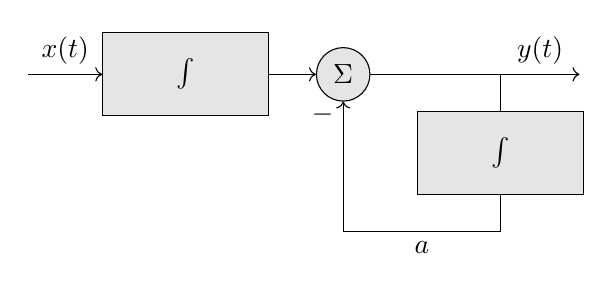
\begin{tikzpicture}[auto]
    \node [input, name=input] at (0,0) {};  	
    \node[block] at (2,0) (block1) {$\int$};
    \node[block] at (6,-1) (block2) {$\int$};
    \node[shape=coordinate] at (6,-2) (input2) {};

    \node [shape=coordinate, name=conn] at (6,0) {};
    \node [shape=coordinate, name=conn2] at (4,-2) {};
    \node [shape=coordinate, name=conn3] at (6,-2) {};
    \node [sum, right of=block1,node distance=2cm] (sum) {$\Sigma$};
    \node [output, right of=conn] (output) {};
    
    \draw (sum) -- (conn);
    \draw (conn) -- (block2);
    \draw (block2) -- (conn3);
    \draw (conn3) -- node {$a$} (conn2);
    \draw [->] (conn2) -| node[pos=0.95] {$-$} (sum);
    \draw [draw,->] (input) -- node {$x(t)$} (block1);
    \draw [->] (block1) -- (sum);
    \draw [->] (conn) -- node {$y(t)$} (output);
  \end{tikzpicture}
\end{center}

We can simplify this block diagram, by noting
\begin{align*}
  y(t) &= -a\int\limits_{-\infty}^t y(\tau)\; d\tau + \int\limits_{-\infty}^t
  x(\tau)\; d\tau\\
  &= \int\limits_{-\infty}^t \left(-a y(\tau) +  x(\tau)\right)\; d\tau\\
\end{align*}
which requires only a single integrator
\begin{center}
  \tikzstyle{block} = [draw, fill=gray!20, rectangle, 
    minimum height=2em, minimum width=2em]
  \tikzstyle{sum} = [draw, fill=gray!20, circle, node distance=1cm]
  \tikzstyle{input} = [coordinate]
  \tikzstyle{output} = [coordinate]
  \tikzstyle{pinstyle} = [pin edge={to-,thin,black}]
  
  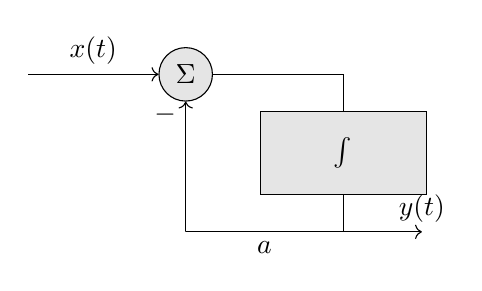
\begin{tikzpicture}[auto]
    \node [input, name=input] at (0,0) {};  	
    \node[block] at (4,-1) (block2) {$\int$};

    \node [shape=coordinate, name=conn] at (4,0) {};
    \node [shape=coordinate, name=conn2] at (2,-2) {};
    \node [shape=coordinate, name=conn3] at (4,-2) {};
    \node [sum, right of=input,node distance=2cm] (sum) {$\Sigma$};
    \node [output, right of=conn3] (output) {};
    
    \draw (sum) -- (conn);
    \draw (conn) -- (block2);
    \draw (block2) -- (conn3);
    \draw (conn3) -- node {$a$} (conn2);
    \draw [->] (conn2) -| node[pos=0.95] {$-$} (sum);
    \draw [draw,->] (input) -- node {$x(t)$} (sum);
    \draw [->] (conn3) -- node[pos=1] {$y(t)$} (output);
  \end{tikzpicture}
\end{center}

The choice of using derivative or integrator blocks is not arbitrary in practice. Derivatives are sensitive to noise at high frequencies (for reasons we will see later in the semester) and so integrators perform much better when implemented in hardware. 

\subsubsection*{Second-Order System}

Now consider the second-order system
\[
\frac{d^2y}{dt^2}(t) + a\frac{dy}{dt}(t)  + by(t)= x(t)
\]
Using a similar process to the first-order system, we can express this as (dropping the limits of integration for clarity):
\[
y(t) = -a \int y(\tau)\; d\tau + \int\int \left( -by(\tau) + x(\tau) \right) \; d\tau^2 
\]
which has the block diagram

\begin{center}
  \tikzstyle{block} = [draw, fill=gray!20, rectangle, 
    minimum height=2em, minimum width=2em]
  \tikzstyle{sum} = [draw, fill=gray!20, circle, node distance=1cm]
  \tikzstyle{input} = [coordinate]
  \tikzstyle{output} = [coordinate]
  \tikzstyle{pinstyle} = [pin edge={to-,thin,black}]
  
  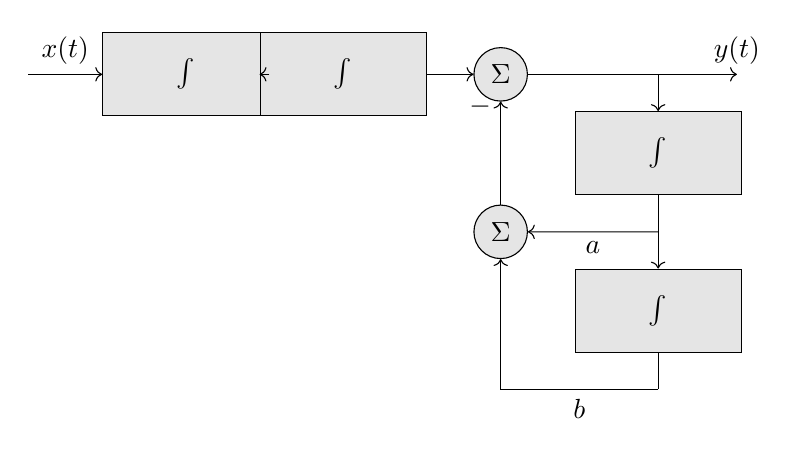
\begin{tikzpicture}[auto]
    \node [input, name=input] at (0,0) {};
    \node [block, right of=input,node distance=2cm] (block1) {$\int$};
    \node [block, right of=block1,node distance=2cm] (block2) {$\int$};
    \node [sum, right of=block2,node distance=2cm] (sum) {$\Sigma$};
    \node [sum, below of=sum,node distance=2cm] (sum2) {$\Sigma$};
    \node[block] at (8,-1) (block3) {$\int$};
    \node[block] at (8,-3) (block4) {$\int$};

    \node [shape=coordinate, name=conn1] at (8,0) {};
    \node [shape=coordinate, name=conn2] at (8,-2) {};
    \node [shape=coordinate, name=conn3] at (8,-4) {};
    \node [shape=coordinate, name=conn4] at (6,-4) {};
    \node [output, right of=conn1] (output) {};

    \draw [->] (input) -- node {$x(t)$} (block1);
    \draw [->] (block1) -- (block2);
    \draw [->] (block2) -- (sum);
    \draw (sum) -- (conn1);
    \draw [->] (conn1) -- (block3);
    \draw (block3) -- (conn2);
    \draw [->] (conn2) -- (block4);
    \draw [->] (conn2) -- node {$a$} (sum2);
    \draw (block4) -- (conn3);
    \draw (conn3) -- node {$b$} (conn4);
    \draw [->] (conn3) -| (sum2);
    \draw [->] (sum2) -- node[pos=0.95] {$-$} (sum);
    \draw [->] (conn1) -- node[pos=1] {$y(t)$} (output);
  \end{tikzpicture}
\end{center}
This is equivalent to two systems in series

\begin{center}
  \tikzstyle{block} = [draw, fill=gray!20, rectangle, 
    minimum height=2em, minimum width=2em]
  \tikzstyle{sum} = [draw, fill=gray!20, circle, node distance=1cm]
  \tikzstyle{input} = [coordinate]
  \tikzstyle{output} = [coordinate]
  \tikzstyle{pinstyle} = [pin edge={to-,thin,black}]
  
  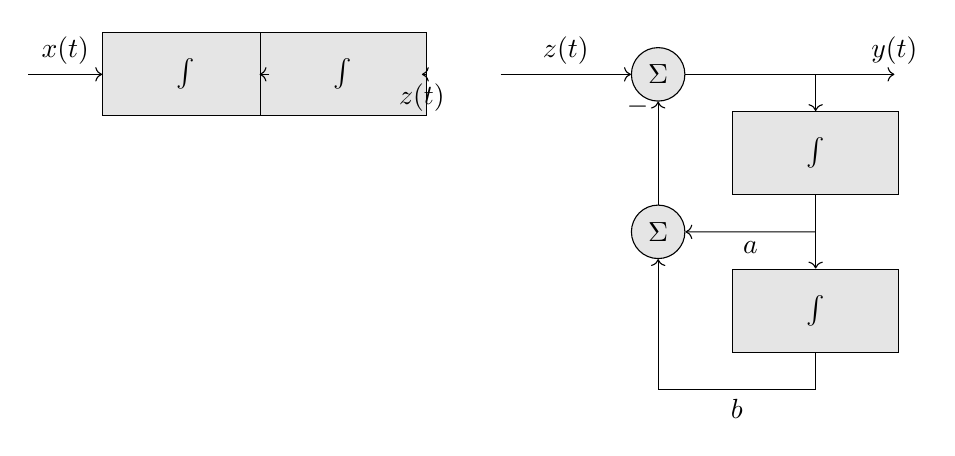
\begin{tikzpicture}[auto]
    \node [input, name=input1] at (0,0) {};
    \node [block, right of=input1,node distance=2cm] (block1) {$\int$};
    \node [block, right of=block1,node distance=2cm] (block2) {$\int$};
    \node [output, right of=block2] (output) {};

    \draw [->] (input1) -- node {$x(t)$} (block1);
    \draw [->] (block1) -- (block2);
    \draw [->] (block2) -- node[pos=1] {$z(t)$} (output);

    \node [input, name=input2] at (6,0) {};
    \node [sum, right of=input2,node distance=2cm] (sum) {$\Sigma$};
    \node [sum, below of=sum,node distance=2cm] (sum2) {$\Sigma$};
    \node[block] at (10,-1) (block3) {$\int$};
    \node[block] at (10,-3) (block4) {$\int$};

    \node [shape=coordinate, name=conn1] at (10,0) {};
    \node [shape=coordinate, name=conn2] at (10,-2) {};
    \node [shape=coordinate, name=conn3] at (10,-4) {};
    \node [shape=coordinate, name=conn4] at (8,-4) {};
    \node [output, right of=conn1] (output) {};

    \draw [->] (input2) -- node {$z(t)$} (sum);
    \draw (sum) -- (conn1);
    \draw [->] (conn1) -- (block3);
    \draw (block3) -- (conn2);
    \draw [->] (conn2) -- (block4);
    \draw [->] (conn2) -- node {$a$} (sum2);
    \draw (block4) -- (conn3);
    \draw (conn3) -- node {$b$} (conn4);
    \draw [->] (conn3) -| (sum2);
    \draw [->] (sum2) -- node[pos=0.95] {$-$} (sum);
    \draw [->] (conn1) -- node[pos=1] {$y(t)$} (output);
    \end{tikzpicture}
\end{center}

Recall that, from the commutative property of convolution, the order of systems in series can be swapped\\

\begin{center}
\tikzstyle{block} = [draw, fill=gray!20, rectangle, 
    minimum height=2em, minimum width=2em]
  \tikzstyle{sum} = [draw, fill=gray!20, circle, node distance=1cm]
  \tikzstyle{input} = [coordinate]
  \tikzstyle{output} = [coordinate]
  \tikzstyle{pinstyle} = [pin edge={to-,thin,black}]
  
  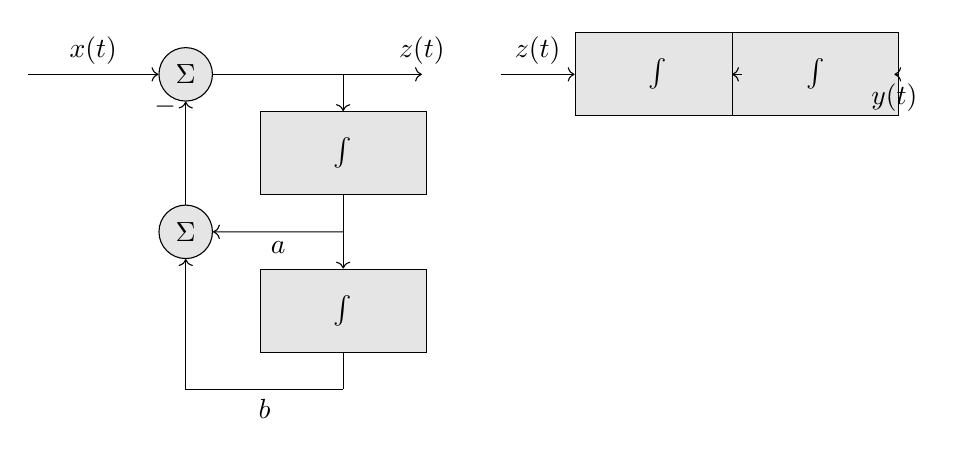
\begin{tikzpicture}[auto]
    \node [input, name=input] at (0,0) {};
    \node [sum, right of=input,node distance=2cm] (sum) {$\Sigma$};
    \node [sum, below of=sum,node distance=2cm] (sum2) {$\Sigma$};
    \node[block] at (4,-1) (block3) {$\int$};
    \node[block] at (4,-3) (block4) {$\int$};

    \node [shape=coordinate, name=conn1] at (4,0) {};
    \node [shape=coordinate, name=conn2] at (4,-2) {};
    \node [shape=coordinate, name=conn3] at (4,-4) {};
    \node [shape=coordinate, name=conn4] at (2,-4) {};
    \node [output, right of=conn1] (output) {};

    \draw [->] (input) -- node {$x(t)$} (sum);
    \draw (sum) -- (conn1);
    \draw [->] (conn1) -- (block3);
    \draw (block3) -- (conn2);
    \draw [->] (conn2) -- (block4);
    \draw [->] (conn2) -- node {$a$} (sum2);
    \draw (block4) -- (conn3);
    \draw (conn3) -- node {$b$} (conn4);
    \draw [->] (conn3) -| (sum2);
    \draw [->] (sum2) -- node[pos=0.95] {$-$} (sum);
    \draw [->] (conn1) -- node[pos=1] {$z(t)$} (output);

    \node [input, name=input] at (6,0) {};
    \node [block, right of=input,node distance=2cm] (block1) {$\int$};
    \node [block, right of=block1,node distance=2cm] (block2) {$\int$};
    \node [output, right of=block2] (output) {};

    \draw [->] (input) -- node {$z(t)$} (block1);
    \draw [->] (block1) -- (block2);
    \draw [->] (block2) -- node[pos=1] {$y(t)$} (output);
  \end{tikzpicture}
\end{center}
We then note that the signal $z$ and the output of the integrator blocks are the same in both systems so that they can be combined into a single block diagram as follows, reducing the number of integrators by two

\begin{center}
  \tikzstyle{block} = [draw, fill=gray!20, rectangle, 
    minimum height=2em, minimum width=2em]
  \tikzstyle{sum} = [draw, fill=gray!20, circle, node distance=1cm]
  \tikzstyle{input} = [coordinate]
  \tikzstyle{output} = [coordinate]
  \tikzstyle{pinstyle} = [pin edge={to-,thin,black}]
  
  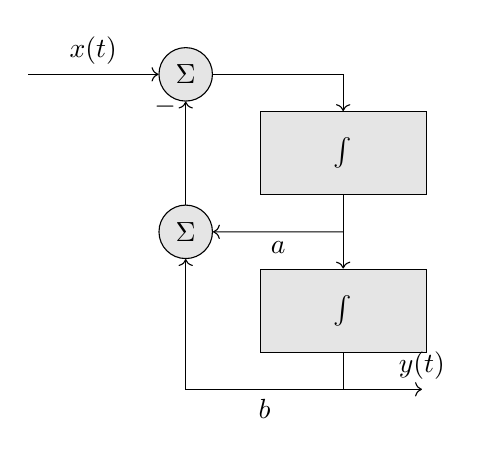
\begin{tikzpicture}[auto]
    \node [input, name=input] at (0,0) {};
    \node [sum, right of=input,node distance=2cm] (sum) {$\Sigma$};
    \node [sum, below of=sum,node distance=2cm] (sum2) {$\Sigma$};
    \node[block] at (4,-1) (block3) {$\int$};
    \node[block] at (4,-3) (block4) {$\int$};

    \node [shape=coordinate, name=conn1] at (4,0) {};
    \node [shape=coordinate, name=conn2] at (4,-2) {};
    \node [shape=coordinate, name=conn3] at (4,-4) {};
    \node [shape=coordinate, name=conn4] at (2,-4) {};
    \node [output, right of=conn3] (output) {};

    \draw [->] (input) -- node {$x(t)$} (sum);
    \draw (sum) -- (conn1);
    \draw [->] (conn1) -- (block3);
    \draw (block3) -- (conn2);
    \draw [->] (conn2) -- (block4);
    \draw [->] (conn2) -- node {$a$} (sum2);
    \draw (block4) -- (conn3);
    \draw (conn3) -- node {$b$} (conn4);
    \draw [->] (conn3) -| (sum2);
    \draw [->] (sum2) -- node[pos=0.95] {$-$} (sum);
    \draw [->] (conn3) -- node[pos=1] {$y(t)$} (output);
  \end{tikzpicture}
\end{center}

\subsection{Implementing a System in Hardware}

One of the most powerful uses of block diagrams is the implementation of a CT system in hardware. As we shall see later in the semester, designing CT systems for a particular purpose leads to a mathematical description that is equivalent to either an impulse response, or a LCCDE. We have seen how these can be represented as block diagrams. Once we have reduced a system to blocks consisting of simple operations, we can then convert the block diagram to a circuit.

\begin{tabular}{cc}

  Block & Typical Circuit\\
  \hline
  \tikzstyle{block} = [draw, fill=gray!20, rectangle, 
    minimum height=2em, minimum width=2em]
  \tikzstyle{sum} = [draw, fill=gray!20, circle, node distance=1cm]
  \tikzstyle{input} = [coordinate]
  \tikzstyle{output} = [coordinate]
  \tikzstyle{pinstyle} = [pin edge={to-,thin,black}]
  
  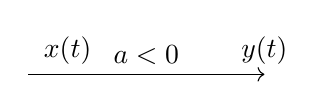
\begin{tikzpicture}[auto]
    \node [input, name=input] at (0,0) {};
    \node [shape=coordinate, name=signal1] at (1,0) {};
    \node [shape=coordinate, name=signal2] at (2,0) {};
    \node [output, right of=signal2] (output) {};

    \draw (input) -- node {$x(t)$} (signal1);
    \draw (signal1) -- node {$a < 0$} (signal2);
    \draw [->] (signal2) -- node[pos=1] {$y(t)$} (output);
  \end{tikzpicture}  

  &
  \begin{circuitikz}[american voltages,scale=0.8, every node/.style={transform shape}]
    \draw
    (5,3.5) node[op amp] (opamp1) {}
    (0,4) to[R,l=$R_1$,o-] (4,4)
    (4,4) to[short] (opamp1.-)
    (opamp1.+) to[short] (3.8,2) 
    (0,2) to[short,o-o] (8,2)
    (opamp1.out) to[short] (6.2,5)
    (3.5,5) to[R,l=$R_2$] (6.2,5)
    (3.5,4) to[short] (3.5,5)
    (opamp1.out) to[short,-o] (8,3.5)
    (0,4) to[open, v=$x(t)$] (0,2)
    (8,3.5) to[open, v=$y(t)$] (8,2);
  \end{circuitikz}
  \\[2em]
  
  \tikzstyle{block} = [draw, fill=gray!20, rectangle, 
    minimum height=2em, minimum width=2em]
  \tikzstyle{sum} = [draw, fill=gray!20, circle, node distance=1cm]
  \tikzstyle{input} = [coordinate]
  \tikzstyle{output} = [coordinate]
  \tikzstyle{pinstyle} = [pin edge={to-,thin,black}]
  
  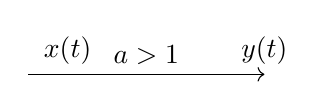
\begin{tikzpicture}[auto]
    \node [input, name=input] at (0,0) {};
    \node [shape=coordinate, name=signal1] at (1,0) {};
    \node [shape=coordinate, name=signal2] at (2,0) {};
    \node [output, right of=signal2] (output) {};

    \draw (input) -- node {$x(t)$} (signal1);
    \draw (signal1) -- node {$a > 1$} (signal2);
    \draw [->] (signal2) -- node[pos=1] {$y(t)$} (output);
  \end{tikzpicture}  
  &
  \begin{circuitikz}[american voltages,scale=0.8, every node/.style={transform shape}]
    \draw
    (7,3.5) node[op amp] (opamp1) {}
    (4,0) to[short,o-o] (12,0)
    (4,4) to[short,o-] (opamp1.-)
    (opamp1.+) to[short] (5.8,1.75)
    (5.8,1.75) to[short] (8.2,1.75)
    (opamp1.out) to[R, l=$R_1$] (8.2,1.75)
    (8.2,1.75) to[R, l=$R_2$] (8.2,0)
    (opamp1.out) to[short, -o] (12,3.5)
    (4,4) to[open, v=$x(t)$] (4,0)
    (12,3.5) to[open, v=$y(t)$] (12,0);
  \end{circuitikz}
  \\[2em]

      \tikzstyle{block} = [draw, fill=gray!20, rectangle, 
        minimum height=2em, minimum width=2em]
      \tikzstyle{sum} = [draw, fill=gray!20, circle, node distance=1cm]
      \tikzstyle{input} = [coordinate]
      \tikzstyle{output} = [coordinate]
      \tikzstyle{pinstyle} = [pin edge={to-,thin,black}]
      
      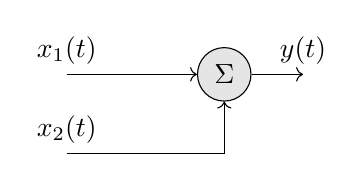
\begin{tikzpicture}[auto]
        \node [input, name=input1] at (0,0) {};
        \node [input, name=input2] at (0,-1) {};
        \node [sum] at (2,0) (sum1) {$\Sigma$};
        \node [output, right of=sum1] (output) {};
        
        \draw [->] (input1) -- node[pos=0] {$x_1(t)$} (sum1);
        \draw [->] (input2) -| node[pos=0] {$x_2(t)$} (sum1);
        \draw [->] (sum1) -- node[pos=1] {$y(t)$} (output);
      \end{tikzpicture}  
    &
      \begin{circuitikz}[american voltages,scale=0.8, every node/.style={transform shape}]
    \draw
    (9,3.5) node[op amp] (opamp1) {}
    (2,0) to[short,o-o] (12,0)
    (2,4) to[short,o-] (5,4)
    (4.5,2) to[short,o-] (5,2)
    (5,4) to[R, l=$R$] (7,4)
    (5,2) to[R, l=$R$] (7,2)
    (7,2) to[short] (7,4)
    (7,4) to[short] (opamp1.-)
    (opamp1.+) to[short] (7.8,1.75)
    (7.8,1.75) to[short] (10.2,1.75)
    (opamp1.out) to[short] (10.2,1.75)
    (opamp1.out) to[short, -o] (12,3.5)
    (2,4) to[open, v=$x_1(t)$] (2,0)
    (4.5,2) to[open, v=$x_2(t)$] (4.5,0)
    (12,3.5) to[open, v=$y(t)$] (12,0);
  \end{circuitikz}
  \\[2em]
      

  \tikzstyle{block} = [draw, fill=gray!20, rectangle, 
    minimum height=2em, minimum width=2em]
  \tikzstyle{sum} = [draw, fill=gray!20, circle, node distance=1cm]
  \tikzstyle{input} = [coordinate]
  \tikzstyle{output} = [coordinate]
  \tikzstyle{pinstyle} = [pin edge={to-,thin,black}]
  
  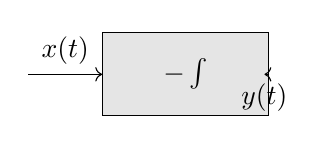
\begin{tikzpicture}[auto]
    \node [input, name=input] at (0,0) {};
    \node[block] at (2,0) (block1) {$-\int$};
    \node [output, right of=block1] (output) {};

    \draw [->] (input) -- node {$x(t)$} (block1);
    \draw [->] (block1) -- node[pos=1] {$y(t)$} (output);
  \end{tikzpicture}  

  &
    \begin{circuitikz}[american voltages,scale=0.8, every node/.style={transform shape}]
    \draw
    (5,3.5) node[op amp] (opamp1) {}
    (0,4) to[R,l=$R$,o-] (4,4)
    (4,4) to[short] (opamp1.-)
    (opamp1.+) to[short] (3.8,2) 
    (0,2) to[short,o-o] (8,2)
    (opamp1.out) to[short] (6.2,5)
    (3.5,5) to[C,l=$C$] (6.2,5)
    (3.5,4) to[short] (3.5,5)
    (opamp1.out) to[short,-o] (8,3.5)
    (0,4) to[open, v=$x(t)$] (0,2)
    (8,3.5) to[open, v=$y(t)$] (8,2);
    \end{circuitikz}\\
    \hline
\end{tabular}

\newpage
\subsection*{Solved Problems}

\begin{enumerate}
\item Consider a system with the following block diagram:
\begin{center}
  \tikzstyle{block} = [draw, fill=gray!20, rectangle, 
    minimum height=2em, minimum width=2em]
  \tikzstyle{sum} = [draw, fill=gray!20, circle, node distance=1cm]
  \tikzstyle{input} = [coordinate]
  \tikzstyle{output} = [coordinate]
  \tikzstyle{pinstyle} = [pin edge={to-,thin,black}]
  
  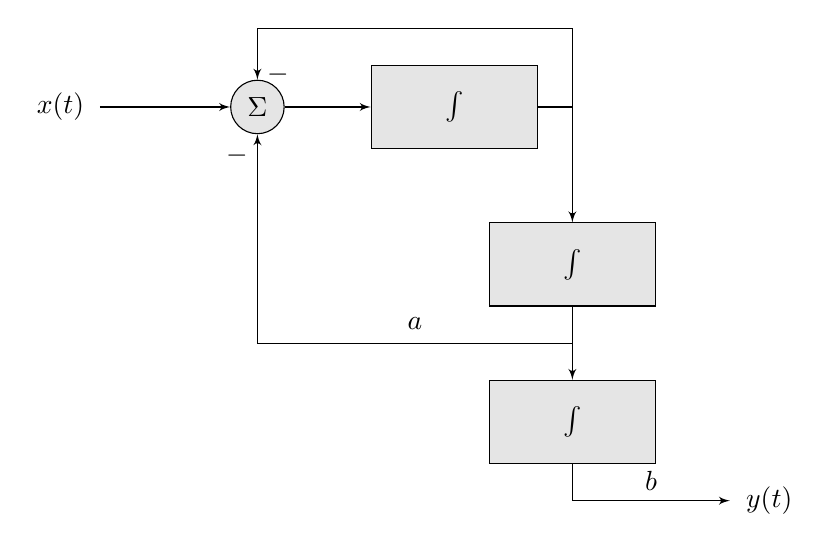
\begin{tikzpicture}[auto, node distance=2cm,>=latex',scale=1, every node/.style={transform shape}]
    \node [input, name=input] at (0,0) {};  	
    \node [block] at (4.5,0) (block1) {$\int$};
    \node [sum] at (2,0) (sum) {$\Sigma$};
    \node [output, name=feedback] at (6,0) {};  	
    \node [output, name=feedback2] at (6,1) {};  	
    \node [output, name=output] at (8,-5) {};  	
    \node [block] at (6,-2) (block2) {$\int$};
    \node [output, name=output2] at (6,-3) {};  	
    \node [block] at (6,-4) (block3) {$\int$};
    \node [output, name=output3] at (6,-5) {};  	
    \draw [->] (input) --  (sum);
    \draw [->] (sum) -- (block1);
    \draw (block1) -- (feedback);
    \draw (feedback) -- (feedback2);
    \draw [->] (feedback2) -| node[pos=0.95] {$-$} (sum);
    \draw [->] (output3) -- node {$b$} (output);
    \draw [->] (feedback) -- (block2);
    \draw [->] (block2) -- (block3);
    \draw [->] (output2) -| node[pos=0.95] {$-$} (sum);
    \draw (block3) -- (output3);
    \draw node at (-0.5,0) {$x(t)$};
    \draw node at (8.5,-5) {$y(t)$};
    \draw node at (4,-2.75) {$a$};
  \end{tikzpicture}
\end{center}

Determine the differential equation representation of this system.\\[1em]


\textbf{Solution:} We can convert this back to a differential equation representation as follows. First label the output of each block as a signal (called the internal states of the system), which we denote as $u(t)$, $v(t)$, $w(t)$, and $z(t)$ below.

\begin{center}
  \tikzstyle{block} = [draw, fill=gray!20, rectangle, 
    minimum height=2em, minimum width=2em]
  \tikzstyle{sum} = [draw, fill=gray!20, circle, node distance=1cm]
  \tikzstyle{input} = [coordinate]
  \tikzstyle{output} = [coordinate]
  \tikzstyle{pinstyle} = [pin edge={to-,thin,black}]
  
  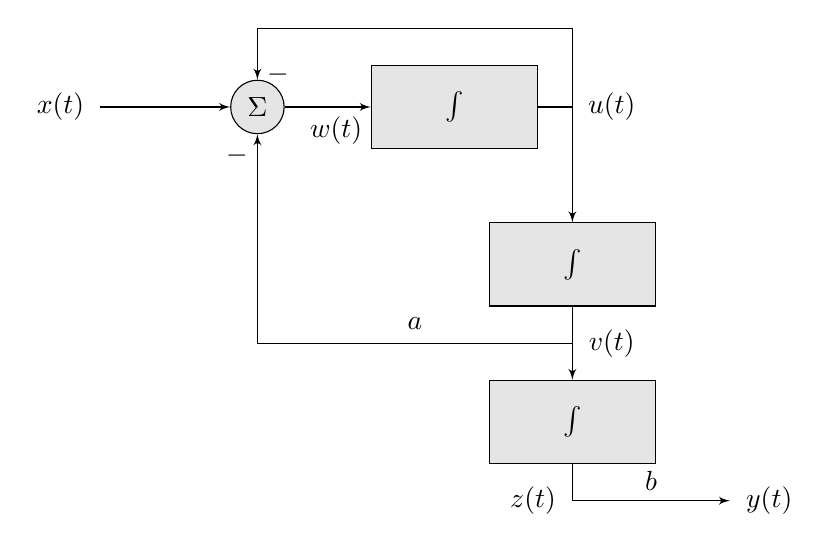
\begin{tikzpicture}[auto, node distance=2cm,>=latex',scale=1, every node/.style={transform shape}]
    \node [input, name=input] at (0,0) {};  	
    \node [block] at (4.5,0) (block1) {$\int$};
    \node [sum] at (2,0) (sum) {$\Sigma$};
    \node [output, name=feedback] at (6,0) {};  	
    \node [output, name=feedback2] at (6,1) {};  	
    \node [output, name=output] at (8,-5) {};  	
    \node [block] at (6,-2) (block2) {$\int$};
    \node [output, name=output2] at (6,-3) {};  	
    \node [block] at (6,-4) (block3) {$\int$};
    \node [output, name=output3] at (6,-5) {};  	
    \draw [->] (input) --  (sum);
    \draw [->] (sum) -- (block1);
    \draw (block1) -- (feedback);
    \draw (feedback) -- (feedback2);
    \draw [->] (feedback2) -| node[pos=0.95] {$-$} (sum);
    \draw [->] (output3) -- node {$b$} (output);
    \draw [->] (feedback) -- (block2);
    \draw [->] (block2) -- (block3);
    \draw [->] (output2) -| node[pos=0.95] {$-$} (sum);
    \draw (block3) -- (output3);
    \draw node at (-0.5,0) {$x(t)$};
    \draw node at (8.5,-5) {$y(t)$};
    \draw node at (4,-2.75) {$a$};
    \draw node at (6.5,0) {$u(t)$};
    \draw node at (6.5,-3) {$v(t)$};
    \draw node at (3,-0.3) {$w(t)$};
    \draw node at (5.5,-5) {$z(t)$};
  \end{tikzpicture}
\end{center}
Now we can read off the input-output relationships moving from input to output. Starting with the output of the summation
\[
w(t) = x(t) - u(t) -a\,v(t) \; .
\]
The outputs of each integrator are:
\[
u(t) = \int\limits_{-\infty}^t w(\tau) \; d\tau\;, \;
v(t) = \int\limits_{-\infty}^t u(\tau) \; d\tau\;, \mbox{ and }\;
z(t) = \int\limits_{-\infty}^t v(\tau) \; d\tau
\]
or equivalently
\[
\frac{du}{dt}(t) = w(t)\;,\; \frac{dv}{dt}(t) = u(t)\; ,\; \mbox{ and }\; \frac{dz}{dt}(t) = v(t)
\]
Finally, the output is:
\[
y(t) = b\, z(t)\; .
\]
We now do a series of derivatives and substitutions
\begin{align*}
  y(t) &= b\, z(t)\\
  \frac{dy}{dt}(t) &= b\, \frac{dz}{dt}(t)\\
  &= b\, v(t)\\
  \frac{d^2y}{dt^2}(t) &= b\, \frac{dv}{dt}(t)\\
  &= b\, u(t)\\
  \frac{d^3y}{dt^3}(t) &= b\, \frac{du}{dt}(t)\\
  &= b\, w(t)\\
  &= b\left( x(t) - u(t) -a\,v(t)\right)
\end{align*}
Rearranging the last equation to isolate the input on the right hand side gives
\[
\frac{d^3y}{dt^3}(t) + b\,u(t) +ab\,v(t) = b\,x(t)\; \mbox{ (Eqn.~1)}
\]
We can now note from above
\[
u(t) = \frac{dv}{dt}(t) =  \frac{d^2z}{dt^2}(t) = \frac{1}{b} \frac{d^2y}{dt^2}(t) \mbox{ and }
\]
\[
v(t) = \frac{dz}{dt}(t) = \frac{1}{b} \frac{dy}{dt}(t)\; .
\]
Substituting these back into Eqn.~1 gives
\[
\frac{d^3y}{dt^3}(t) + \frac{d^2y}{dt^2}(t) +a\,\frac{dy}{dt}(t) = b\,x(t)
\]
Which is a LCCDE.\\
$\blacksquare$
\end{enumerate}


\newpage
\chapter{DT Block Diagrams}

\section{The Four Basic Motifs}

Block diagrams of DT systems are similar to CT systems.

The four motifs are:

\begin{itemize}
\item A single block.\\[1em] 
\begin{tikzpicture}[auto, node distance=2cm,>=latex',scale=1, every node/.style={transform shape}]
    \node [input, name=input] {};
    \node [block, right of=input] (system) {$\mathcal{S}_1$};
    \node [output, right of=system] (output) {};


    \draw [draw,->] (input) -- node {$x[n]$} (system);
    \draw [->] (system) -- node {$y[n]$} (output);
\end{tikzpicture}

\item A {\it series} connection of two blocks\\[1em]
\begin{tikzpicture}[auto, node distance=2cm,>=latex',scale=1, every node/.style={transform shape}]

    \node [input, name=input] {};
    \node [block, right of=input] (system1) {$\mathcal{S}_1$};
    \node [block, right of=system1,node distance=4cm] (system2) {$\mathcal{S}_2$};
    \node [output, right of=system2] (output) {};


    \draw [draw,->] (input) -- node {$x[n]$} (system1);
    \draw [->] (system1) -- (system2);
    \draw [->] (system2) -- node {$y[n]$} (output);
\end{tikzpicture}
\item A {\it parallel} connection of two blocks\\[1em]
\begin{tikzpicture}[auto, node distance=2cm,>=latex',scale=1, every node/.style={transform shape}]

    \node[shape=coordinate] at (1,1) (input1) {};
    \node[block] at (3,1) (block1) {$\mathcal{S}_1$};
    \node[shape=coordinate] at ($(block1.east)+(0.5,0)$) (output1) {};
    \draw[->] (input1) -- (block1);
    \draw (block1) -- (output1);

    \node[shape=coordinate] at (1,-1) (input2) {};
    \node[block] at (3,-1) (block2) {$\mathcal{S}_2$};
    \node[shape=coordinate] at ($(block2.east)+(0.5,0)$) (output2) {};
    \draw[->] (input2) -- (block2);
    \draw (block2) -- (output2);

    \node [input, name=input] at (0,0) {};  	
    \node [input, name=conn] at (1,0) {};
    \draw (conn) -- (input1);
    \draw (conn) -- (input2);
    \node [sum, right of=input,node distance=5cm] (sum) {$\Sigma$};
    \draw [->] (output1) -| (sum);
    \draw [->] (output2) -| (sum);

    \draw [draw] (input) -- node {$x[n]$} (conn);
    \node [output, right of=sum] (output) {};
    \draw [->] (sum) -- node {$y[n]$} (output);
\end{tikzpicture}

\item A {\it feedback} connection\\[1em]
\begin{tikzpicture}[auto, node distance=2cm,>=latex',scale=1, every node/.style={transform shape}]
    \node[block] at (4,0) (block1) {$\mathcal{S}_1$};

    \node[block] at (4,-2) (block2) {$\mathcal{S}_2$};
    \node[shape=coordinate] at (6,-2) (input2) {};

    \node [input, name=input] at (0,0) {};  	
    \node [shape=coordinate, name=conn] at (6,0) {};
    \draw (block1) -- (conn);
    \draw (conn) -- (input2);
    \draw [->] (input2) -- (block2);

    \node [sum, right of=input,node distance=2cm] (sum) {$\Sigma$};
    \draw [->] (block2) -| node[pos=0.95] {$-$} (sum);

    \draw [draw,->] (input) -- node {$x[n]$} (sum);
    \draw [->] (sum) -- (block1);
    \node [output, right of=conn] (output) {};
    \draw [->] (conn) -- node {$y[n]$} (output);
\end{tikzpicture}
\end{itemize}

Note the feedback is negative (the minus sign on the feedback summation input). As in CT, these can be used in various combinations.

\section{Connections to Convolution}

Each subsystem, $\mathcal{S}_i$, can be represented by a basic discrete time-domain operation (e.g. differences, running sums, addition, and scaling) or more generally by its impulse response $h_i[n]$.

For example a block representing an system acting as a delay of one sample is typically drawn as

\begin{center}
  \begin{tikzpicture}[auto, node distance=2cm,>=latex',scale=1, every node/.style={transform shape}]
    \node [input, name=input] {};
    \node [block, right of=input] (system) {$D$};
    \node [output, right of=system] (output) {};
    \draw [draw,->] (input) -- node {$x[n]$} (system);
    \draw [->] (system) -- node[pos=2] {$y[n] = x[n-1]$} (output);
\end{tikzpicture}
\end{center}
This is equivalent to an impulse response $h[n] = \delta[n-1]$ so that it might also be drawn as
\begin{center}
  \begin{tikzpicture}[auto, node distance=2cm,>=latex',scale=1, every node/.style={transform shape}]
    \node [input, name=input] {};
    \node [block, right of=input] (system) {$h[n] = \delta[n-1]$};
    \node [output, right of=system] (output) {};

    \draw [draw,->] (input) -- node {$x[n]$} (system);
    \draw [->] (system) -- node[pos=4] {$y[n] = x[n] * \delta[n-1] = x[n-1]$} (output);
\end{tikzpicture}
\end{center}

Similarly, a block representing an system acting as an advance of one sample is typically drawn as

\begin{center}
  \begin{tikzpicture}[auto, node distance=2cm,>=latex',scale=1, every node/.style={transform shape}]
    \node [input, name=input] {};
    \node [block, right of=input] (system) {$E$};
    \node [output, right of=system] (output) {};
    \draw [draw,->] (input) -- node {$x[n]$} (system);
    \draw [->] (system) -- node[pos=2] {$y[n] = x[n+1]$} (output);
\end{tikzpicture}
\end{center}
This is equivalent to an impulse response $h[n] = \delta[n+1]$ so that it might also be drawn as
\begin{center}
  \begin{tikzpicture}[auto, node distance=2cm,>=latex',scale=1, every node/.style={transform shape}]
    \node [input, name=input] {};
    \node [block, right of=input] (system) {$h[n] = \delta[n+1]$};
    \node [output, right of=system] (output) {};

    \draw [draw,->] (input) -- node {$x[n]$} (system);
    \draw [->] (system) -- node[pos=4] {$y[n] = x[n] * \delta[n+1] = x[n+1]$} (output);
\end{tikzpicture}
\end{center}

We can use the concept of convolution to connect block diagrams to the properties of convolution

\begin{itemize}
\item A single block is equivalent to convolution with the impulse response for that subsystem\\[1em] 
\begin{tikzpicture}[auto, node distance=2cm,>=latex',scale=1, every node/.style={transform shape}]

    \node [input, name=input] {};
    \node [block, right of=input] (system) {$h_1[n]$};
    \node [output, right of=system] (output) {};

    \draw [draw,->] (input) -- node {$x[n]$} (system);
    \draw [->] (system) -- node[pos=2] {$y[n] = h_1[n]*x[n]$} (output);
\end{tikzpicture}

\item Using the associative property, a series connection of two blocks becomes
  \begin{center}
\begin{tikzpicture}[auto, node distance=2cm,>=latex',scale=1, every node/.style={transform shape}]
    % We start by placing the blocks
    \node [input, name=input] {};
    \node [block, right of=input] (system1) {$h_1[n]$};
    \node [block, right of=system1,node distance=4cm] (system2) {$h_2[n]$};
    \node [output, right of=system2] (output) {};

    \draw [draw,->] (input) -- node {$x[n]$} (system1);
    \draw [->] (system1) -- (system2);
    \draw [->] (system2) -- node[pos=3] {$y[n] = \left(h_1[n]*h_2[n]\right)*x[n]$} (output);
\end{tikzpicture}
  \end{center}
  which can be reduced to a single convolution $y[n] = h_3[n]*x[n]$ where $h_3[n] = h_1[n]*h_2[n]$.
\item Using the distributive property, a parallel connection of two blocks becomes
  \begin{center}
\begin{tikzpicture}[auto, node distance=2cm,>=latex',scale=1, every node/.style={transform shape}]

    \node[shape=coordinate] at (1,1) (input1) {};
    \node[block] at (3,1) (block1) {$h_1[n]$};
    \node[shape=coordinate] at ($(block1.east)+(0.5,0)$) (output1) {};
    \draw[->] (input1) -- (block1);
    \draw (block1) -- (output1);

    \node[shape=coordinate] at (1,-1) (input2) {};
    \node[block] at (3,-1) (block2) {$h_2[n]$};
    \node[shape=coordinate] at ($(block2.east)+(0.5,0)$) (output2) {};
    \draw[->] (input2) -- (block2);
    \draw (block2) -- (output2);

    \node [input, name=input] at (0,0) {};  	
    \node [input, name=conn] at (1,0) {};
    \draw (conn) -- (input1);
    \draw (conn) -- (input2);
    \node [sum, right of=input,node distance=5cm] (sum) {$\Sigma$};
    \draw [->] (output1) -| (sum);
    \draw [->] (output2) -| (sum);

    \draw [draw] (input) -- node {$x[n]$} (conn);
    \node [output, right of=sum] (output) {};
    \draw [->] (sum) -- node[pos=3] {$y[n]= \left(h_1[n]*x[n]\right) +  \left(h_2[n]*x[n]\right) =  \left(h_1[n]+h_2[n]\right)*x[n]$} (output);
\end{tikzpicture}  
  \end{center}
  which is equivalent to a single convolution $y[n] = h_3[n]*x[n]$ where $h_3[n] = h_1[n] + h_2[n]$.
\item In the feedback connection let $w[n]$ be the output of the summation
  \begin{center}
\begin{tikzpicture}[auto, node distance=2cm,>=latex',scale=1, every node/.style={transform shape}]
    % We start by placing the blocks
    \node[block] at (4.5,0) (block1) {$h_1[n]$};

    \node[block] at (4,-2) (block2) {$h_2[n]$};
    \node[shape=coordinate] at (6,-2) (input2) {};

    \node [input, name=input] at (0,0) {};  	
    \node [shape=coordinate, name=conn] at (6,0) {};
    \draw (block1) -- (conn);
    \draw (conn) -- (input2);
    \draw [->] (input2) -- (block2);

    \node [sum, right of=input,node distance=2cm] (sum) {$\Sigma$};
    \draw [->] (block2) -| node[pos=0.95] {$-$} (sum);

    \draw [draw,->] (input) -- node {$x[n]$} (sum);
    \draw [->] (sum) -- (block1);
    \node [output, right of=conn] (output) {};
    \draw [->] (conn) -- node {$y[n]$} (output);
    \draw node at (3,0.3) {$w[n]$};
\end{tikzpicture}
  \end{center}
  Then $y[n] = h_1[n]*w[n]$ and $w[n] = x[n] - h_2[n]*y[n]$. Substituting the later into the former gives $y[n] = h_1*(x-h_2[n]*y[n])$. Using the distributive property we get $y[n] = h_1[n]*x[n] - h_1[n]*h_2[n]*y[n]$. Isolating the input on the right-hand side and using $y[n] = \delta[n]*y[n]$ we get
  \[
  y[n] + h_1[n]*h_2[n]*y[n] = \left(\delta[n] + h_1[n]*h_2[n]\right)*y[n] = h_1[n]*x[n] 
  \]
  We can solve this for $y[n]$ using the concept of inverse systems. Let $h_3[n]* \left(\delta[n] + h_1[n]*h_2[n]\right)= \delta[n]$, i.e. $h_3$ is the inverse system of $\delta[n] + h_1[n]*h_2[n]$. Then
  \[
  y[n] = h_3[n]*h_1[n]*x[n]
  \]
\end{itemize}

Recall, when the system is instantaneous (memoryless) the impulse response is $a\delta[n]$ for some constant $a$. This is the same as scaling the signal by $a$. We typically drop the block in such cases and draw the input-output operation as

\begin{center}
\begin{tikzpicture}[auto, node distance=2cm,>=latex',scale=1, every node/.style={transform shape}]
  \node [input, name=input] at (0,0) {};
  \node [output, name=system] at (2,0) {};
  \node [output, name=output] at (4,0) {};
  \draw [draw,->] (input) -- node {$x[n]$} (system);
  \draw [draw,->] (system) -- node[pos=1] {$y[n] = ax[n]$} (output);
  \draw [->] (input) -- node {$a$} (output);
\end{tikzpicture}
\end{center}

These properties allow us to perform transformations, either breaking up a system into subsystems, or reducing a system to a single block.

\begin{example}
  Consider a second-order system system with impulse response
  \[
  h[n] = \left(\frac{1}{2}\right)^n\, u[n] + \left(\frac{3}{4}\right)^n\, u[n]
  \]
  We can express this as a block diagram consisting of two parallel blocks
  \begin{center}
\begin{tikzpicture}[auto, node distance=2cm,>=latex',scale=1, every node/.style={transform shape}]

    \node[shape=coordinate] at (1,1) (input1) {};
    \node[block] at (3,1) (block1) {$h_1[n] = \left(\frac{1}{2}\right)^nu[n]$};
    \node[shape=coordinate] at ($(block1.east)+(0.5,0)$) (output1) {};
    \draw[->] (input1) -- (block1);
    \draw (block1) -- (output1);

    \node[shape=coordinate] at (1,-1) (input2) {};
    \node[block] at (3,-1) (block2) {$h_2[n] = \left(\frac{3}{4}\right)^nu[n]$};
    \node[shape=coordinate] at ($(block2.east)+(0.5,0)$) (output2) {};
    \draw[->] (input2) -- (block2);
    \draw (block2) -- (output2);

    \node [input, name=input] at (0,0) {};  	
    \node [input, name=conn] at (1,0) {};
    \draw (conn) -- (input1);
    \draw (conn) -- (input2);
    \node [sum, right of=input,node distance=5cm] (sum) {$\Sigma$};
    \draw [->] (output1) -| (sum);
    \draw [->] (output2) -| (sum);

    \draw [draw] (input) -- node {$x[n]$} (conn);
    \node [output, right of=sum] (output) {};
    \draw [->] (sum) -- node[pos=1] {$y[n]$} (output);
\end{tikzpicture}
  \end{center}
\end{example}

\section{Connections to LCCDE}

The other DT system representation we have seen are linear, constant-coefficient difference equations. These can be expressed as combinations of advance or delay blocks. This is straightforward compared to the CT system case.

\subsection*{First-Order System}

To illustrate this consider the first-order LCCDE
\[
y[n+1] + ay[n]= x[n+1]
\]
We can solve this for $y[n]$
\[
y[n] = -\frac{1}{a}y[n+1]  + \frac{1}{a}x[n+1]
\]
and can express this as a feedback motif using the advance operator $E$
\begin{center}
  \tikzstyle{block} = [draw, fill=gray!20, rectangle, 
      minimum height=2em, minimum width=2em]
  \begin{tikzpicture}[auto]
    \node [input, name=input] at (0,0) {};
    \node [left of=input] {$x[n]$};
    \node[block, right of=input, node distance=5em] (block1) {$E$};
    \node [sum, right of=block1, node distance=5em] (sum) {$\Sigma$};
    \node[block] at (5,-1) (block2) {$E$};
    \node [shape=coordinate, name=conn] at (6,0) {};
    \node[shape=coordinate] at (7,0) (output) {};
    \node [right of=output] {$y[n]$};
    
    \draw [->] (input) -- node {$\frac{1}{a}$} (block1);
    \draw [->] (block1) -- (sum);
    \draw (sum) -- (conn);
    \draw [->] (conn) -- (output);
    \draw [->] (conn) |- (block2);
    \draw [->] (block2) -| node {$-\frac{1}{a}$} (sum);
  \end{tikzpicture}
\end{center}

Alternatively we could rewrite the difference equation in recursive delay form
\[
y[n] = -ay[n-1] +x[n]
\]
which can be expressed as a block diagram using the delay operator, $D$
\begin{center}
  \tikzstyle{block} = [draw, fill=gray!20, rectangle, 
      minimum height=2em, minimum width=2em]
  \begin{tikzpicture}[auto]
    \node [input, name=input] at (0,0) {};
    \node [left of=input] {$x[n]$};
    \node [sum, right of=input, node distance=5em] (sum) {$\Sigma$};
    \node[block] at (3,-1) (block2) {$D$};
    \node [shape=coordinate, name=conn] at (4,0) {};
    \node[shape=coordinate] at (5,0) (output) {};
    \node [right of=output] {$y[n]$};
    
    \draw [->] (input) -- (sum);
    \draw (sum) -- (conn);
    \draw [->] (conn) -- (output);
    \draw [->] (conn) |- (block2);
    \draw [->] (block2) -| node {$-a$} (sum);
  \end{tikzpicture}
\end{center}

The choice of using advance or delay blocks results in a non-causal or causal (respectively) system. Thus, delay blocks are required for real-time DT system implementations.

\subsection*{Second-Order System}

Now consider the second-order system
\[
y[n+2] + ay[n+1] + by[n] = x[n+2]
\]
Again, writing in recursive delay form 
\[
y[n] = -ay[n-1] - by[n-2] + x[n]
\]
we obtain the block diagram
\begin{center}
  \tikzstyle{block} = [draw, fill=gray!20, rectangle, 
      minimum height=2em, minimum width=2em]
  \begin{tikzpicture}[auto]
    \node [input, name=input] at (0,0) {};
    \node [left of=input] {$x[n]$};
    \node [sum] at (2,0) (sum1) {$\Sigma$};
    \node [block] at (4,-1) (block1) {$D$};
    \node [block] at (4,-3) (block2) {$D$};
    \node [shape=coordinate, name=conn1] at (4,-2) {};
    \node [shape=coordinate, name=conn2] at (4,-4) {};
    \node [sum] at (2,-2) (sum2) {$\Sigma$};
    \node [shape=coordinate, name=conn] at (4,0) {};
    \node [shape=coordinate] at (5,0) (output) {};
    \node [right of=output] {$y[n]$};
    
    \draw [->] (input) -- (sum1);
    \draw (sum1) -- (conn);
    \draw [->] (conn) -- (output);
    \draw [->] (conn) -- (block1);
    \draw (block1) -- (conn1);
    \draw [->] (conn1) -- node {$-a$} (sum2);
    \draw [->] (conn1) -- (block2);
    \draw (block2) -- (conn2);
    \draw [->] (conn2) -| node {$-b$} (sum2);
    \draw [->] (sum2) -- (sum1);
  \end{tikzpicture}
\end{center}

\section{Implementing a DT System}

As in the CT case, one of the most powerful uses of block diagrams is the implementation of a DT system in hardware. As we shall see later in the semester, designing a DT system for a particular purpose leads to a mathematical description that is equivalent to either an impulse response or a LCCDE. We have seen how these can be represented as block diagrams. Once we have reduced a system to blocks consisting of simple operations, we can then convert the block diagram to a digital circuit, implement using a digital signal processor, or write an equivalent program to run on an embedded or general purpose computer.

\begin{tabular}{cc}

  Block & Typical Digital Circuit\\
  \hline
  \tikzstyle{block} = [draw, fill=gray!20, rectangle, 
    minimum height=2em, minimum width=2em]
  \tikzstyle{sum} = [draw, fill=gray!20, circle, node distance=1cm]
  \tikzstyle{input} = [coordinate]
  \tikzstyle{output} = [coordinate]
  \tikzstyle{pinstyle} = [pin edge={to-,thin,black}]
  
  \begin{tikzpicture}[auto]
    \node [input, name=input] at (0,0) {};
    \node [shape=coordinate, name=signal1] at (1,0) {};
    \node [shape=coordinate, name=signal2] at (2,0) {};
    \node [output, right of=signal2] (output) {};

    \draw (input) -- node {$x[n]$} (signal1);
    \draw (signal1) -- node {$a$} (signal2);
    \draw [->] (signal2) -- node[pos=1] {$y[n]$} (output);
  \end{tikzpicture}  

  &
  Multiplier (ALU)
  \\[2em]

  \tikzstyle{block} = [draw, fill=gray!20, rectangle, 
    minimum height=2em, minimum width=2em]
  \tikzstyle{sum} = [draw, fill=gray!20, circle, node distance=1cm]
  \tikzstyle{input} = [coordinate]
  \tikzstyle{output} = [coordinate]
  \tikzstyle{pinstyle} = [pin edge={to-,thin,black}]
  
  \begin{tikzpicture}[auto]
    \node [input, name=input1] at (0,0) {};
    \node [input, name=input2] at (0,-1) {};
    \node [sum] at (2,0) (sum1) {$\Sigma$};
    \node [output, right of=sum1] (output) {};
    
    \draw [->] (input1) -- node[pos=0] {$x_1[n]$} (sum1);
    \draw [->] (input2) -| node[pos=0] {$x_2[n]$} (sum1);
    \draw [->] (sum1) -- node[pos=1] {$y[n]$} (output);
  \end{tikzpicture}  
  &
  Adder (ALU)
  \\[2em]
      
  \tikzstyle{block} = [draw, fill=gray!20, rectangle, 
    minimum height=2em, minimum width=2em]
  \tikzstyle{sum} = [draw, fill=gray!20, circle, node distance=1cm]
  \tikzstyle{input} = [coordinate]
  \tikzstyle{output} = [coordinate]
  \tikzstyle{pinstyle} = [pin edge={to-,thin,black}]
  
  \begin{tikzpicture}[auto]
    \node [input, name=input] at (0,0) {};
    \node[block] at (2,0) (block1) {$D$};
    \node [output, right of=block1] (output) {};

    \draw [->] (input) -- node {$x[n]$} (block1);
    \draw [->] (block1) -- node[pos=1] {$y[n]$} (output);
  \end{tikzpicture}  

  &
  Shift Register\\
  \hline
\end{tabular}

\begin{example} The following C++ code implements the second order system given by
\begin{center}
  \tikzstyle{block} = [draw, fill=gray!20, rectangle, 
      minimum height=2em, minimum width=2em]
  \begin{tikzpicture}[auto]
    \node [input, name=input] at (0,0) {};
    \node [left of=input] {$x[n]$};
    \node [sum] at (2,0) (sum1) {$\Sigma$};
    \node [block] at (4,-1) (block1) {$D$};
    \node [block] at (4,-3) (block2) {$D$};
    \node [shape=coordinate, name=conn1] at (4,-2) {};
    \node [shape=coordinate, name=conn2] at (4,-4) {};
    \node [sum] at (2,-2) (sum2) {$\Sigma$};
    \node [shape=coordinate, name=conn] at (4,0) {};
    \node [shape=coordinate] at (5,0) (output) {};
    \node [right of=output] {$y[n]$};
    
    \draw [->] (input) -- (sum1);
    \draw (sum1) -- (conn);
    \draw [->] (conn) -- (output);
    \draw [->] (conn) -- (block1);
    \draw (block1) -- (conn1);
    \draw [->] (conn1) -- node {$-\frac{1}{2}$} (sum2);
    \draw [->] (conn1) -- (block2);
    \draw (block2) -- (conn2);
    \draw [->] (conn2) -| node {$-\frac{1}{9}$} (sum2);
    \draw [->] (sum2) -- (sum1);
  \end{tikzpicture}
\end{center}
using floating point calculations. It assumes the current input is obtained via the function \texttt{read}, and the output written using the function \texttt{write}. The delayed values of the output are stored in the array \texttt{buffer} and are initialized to zero ("at rest" prior to application of the input).
\begin{verbatim}
double buffer[2] = {0.0,0.0};
while(true){
  double x = read();
  double y = -0.5*buffer[1] - buffer[0]/9.0 + x;
  write(y);
  buffer[0] = buffer[1];
  buffer[1] = y;
}
\end{verbatim}
Note in real applications it is common to replace the floating point calculations with fixed-width (scaled integer) ones.
$\blacksquare$
\end{example}



\end{document}
